\documentclass[rascunho, oneside]{fei}

\usepackage[utf8]{inputenc}
\usepackage{amsthm}
\usepackage{caption}
\usepackage{subcaption}
\usepackage{multirow}% http://ctan.org/pkg/multirow
\usepackage{hhline}% http://ctan.org/pkg/hhline

\graphicspath{{images/}}

\newtheorem{mydef}{Definição}

\hypersetup{
pdftitle={Classificador Bayesiano de Perfil do Usuário utilizando a Aproximação do Robô},
pdfauthor={Andrey Araujo Masiero},
pdfkeywords={\emph{Proxemics};}{Redes Bayesianas;}{Robótica Social;}{Interação Humano-Robô;}{QGSIM;},
}

\author{Andrey Araujo Masiero}
\title{Classificador Bayesiano de Perfil do Usuário utilizando a Aproximação do Robô}

\addbibresource{biblio.bib}

\begin{document}

%!TEX root=Principal.tex
\maketitle{}

\begin{folhaderosto}
Tese de Doutorado apresentada ao Centro Universitário da FEI para obtenção do título de Doutor em Engenharia Elétrica, orientado pelo Prof. Dr. Plinio Thomaz Aquino Junior e coorientado pelo Prof. Dr. Flavio Tonidandel.
\end{folhaderosto}

%\fichacatalografica
%\folhadeaprovacao

%%%%%%%%%%%%%%%%%%%%%%%%%%%%%%%%%%%%%%%%%%%%%%%%%%%%%%%%%

\dedicatoria{A Deus e a minha família que são o alicerce de minha vida.}

%%%%%%%%%%%%%%%%%%%%%%%%%%%%%%%%%%%%%%%%%%%%%%%%%%%%%%%%%
\begin{agradecimentos}
Em primeiro lugar gostaria de agradecer a Deus, que sempre me trouxe sabedoria e luz, mesmo nos momentos difíceis dessa jornada e de tantas outras.

À minha mãe Kathia, que desde o primeiro momento me apoiou e incentivou, mesmo quando tudo parecia impossível e eu não conseguia ver a luz no fim do túnel.

À minha irmã Andressa, que me suportou quando fiquei exaltado de felicidade ou tristeza perante as dificuldades.

À minha companheira Marília, que sem seu apoio, compreensão, dedicação à nós durante todo o período mais difícil dessa tese esteve ao meu lado sem se quer reclamar.

Aos meus avós, Hélio e Rachel, que mesmo não presentes em carne, continuam iluminando minha vida e me guiam pelos caminhos que percorro deixando a sensação de sempre estar seguro.

Ao professor e orientador Plinio Thomaz Aquino Junior, que me auxilia a direcionar nos caminhos ao longo da jornada acadêmica e pessoal, com seus sábios conselhos e cumplicidade, fortalecendo a parceira a cada momento nesses últimos anos.

Ao professor e coorientador Flavio Tonidandel, que ajudou a tornar esse trabalho possível, com seus conselhos e ensinamentos, além de sempre puxar a minha orelha quando algo estava estranho ou elogiar sempre que eu conseguia um bom resultado. Tudo isso faz com que nossa parceria seja majestosa, desde a época do mestrado.

Aos professores da FEI, que compartilharam ao longo desse período seus conhecimentos e amizade, ajudando na evolução desse trabalho e também a minha como pessoa.

Aos meus amigos, que sem esse laço seria impossível avançar mais um passo neste caminho cheio de curvas. Os momentos de descontração, de discussão, almoços e principalmente cafés foram e são de extrema importância para nos ajudar a andar no caminho chamado vida.

E por fim a todos que de alguma maneira contribuíram para mais essa conquista.

\end{agradecimentos}

%%%%%%%%%%%%%%%%%%%%%%%%%%%%%%%%%%%%%%%%%%%%%%%%%%%%%%%%%
\epigrafe{In life, unlike chess, the game continues after checkmate.}{Isaac Asimov, 1988}

%%%%%%%%%%%%%%%%%%%%%%%%%%%%%%%%%%%%%%%%%%%%%%%%%%%%%%%%%
\begin{resumo}
A evolução da tecnologia torna-se cada vez mais evidente com o passar dos anos. As pessoas possuem computadores portáteis menores e com melhor configuração, \emph{tablets}, aparelhos de telefonia móvel inteligentes interligados com relógios e também robôs que possuem tarefas específicas como aspirar o pó da casa ou monitorar o ambiente a partir de um determinado ponto. Contudo, o robô inserido no ambiente doméstico ou pessoal atual, é apenas mais um dispositivo tecnológico que a pessoa possui. Caso um robô autônomo capaz de realizar diversas tarefas domésticas e de cuidados pessoais médicos seja inserido nesse ambiente e ainda ele realize interações através de voz, gestos e toque com o ser humano, o sentimento a partir desse momento não seria mais de um dispositivo tecnológico no ambiente. Existe uma possibilidade do ser humano ficar de uma certa maneira desconfortável com a presença do robô. Considerando a situação de desconforto do ser humano com o robô, essa tese propõem uma metodologia que mapeia o conjunto de ações que o robô é capaz de executar visando a maximização da probabilidade de uma interação humano-robô com maior qualidade, baseando-se no comportamento e características do indivíduo. A partir do mapeamento de comportamento da pessoa é possível determinar o comportamento que o robô deve ter para proporcionar uma situação confortável para a interação com o ser humano. Como resultado espera-se um \emph{framework} que possa aprender e analisar o comportamento do ser humano e que também seja capaz de transferir esse conhecimento com o robô inserido no ambiente, aumentando a eficácia da interação entre humanos e robôs.

\palavraschave{Robótica Social, Proxemics, Aprendizado de Máquina, Interação Humano-Robô}
\end{resumo}
%%%%%%%%%%%%%%%%%%%%%%%%%%%%%%%%%%%%%%%%%%%%%%%%%%%%%%%%%
\begin{abstract}
The technology's evolution has increased over the years. People have smaller laptops with better set up, tablets, smartphones interconnected with watches and also robots, which have specific tasks such as vacuuming or monitoring the environment from a certain point. However, the robot inserted into the current household or staff, is just another technological device that the person has. If an autonomous robot, able to perform various household chores and personal care doctors to be entered in this environment and still perform it interactions via voice, gestures and touch with the human being, the feeling would be no more than a technological device into the environment. There is a possibility of human beings in a way become uncomfortable with the presence of the robot. Considering the uncomfortable situation of the human being with the robot, this thesis proposes a methodology that maps the set of actions that the robot is able to perform in order to maximize the likelihood of human-robot interaction with higher quality, based on behavior and characteristics of the individual. From the behavior of the person mapping you can determine the behavior that the robot should have to provide a comfortable situation for interaction with humans. As a result we expect a framework that can learn and analyze the human behavior and also be able to transfer this knowledge to the robot inserted in the environment, increasing the effectiveness of the interaction between humans and robots.

\keywords{Social Robotic, Proxemics, Machine Learning, Human-Robot Interaction}
\end{abstract}



%%%%%%%%%%%%%%%%%%%%%%%%%%%%%%%%%%%%%%%%%%%%%%%%%%%%%%%%%
\listoffigures
% \listoftables
%\listofalgorithms
%\printglossaries

\tableofcontents

%%%%%%%%%%%%%%%%%%%%%%%%%%%%%%%%%%%%%%%%%%%%%%%%%%%%%%%%%

%!TEX root=Principal.tex
\chapter{INTRODUÇÃO}
\label{cap:introducao}
Com o passar dos anos é possível acompanhar a evolução dos sistemas computacionais, como por exemplo os telefones móveis, os computadores pessoais e portáteis, as televisões, e também os robôs pessoais, como o aspirador de pó iRobot Roomba\footnote{http://www.irobot.com/For-the-Home/Vacuum-Cleaning/Roomba.aspx} e o assistente pessoal JIBO\footnote{https://www.jibo.com/}. A evolução dos telefones móveis inteligentes mostra uma alta capacidade na realização de processamento de informações para executar diversas tarefas no dia a dia. Os componentes eletrônicos que compõem os aparelhos também diminuiram o tamanho. Isso permite que os aparelhos sejam mais finos, leves e com maior capacidade de processamento. Há também a inserção de robôs móveis em ambientes sociais, como as casas, hospitais e hotéis, unidos ao cenário da \emph{internet} das coisas. Entretanto, os robôs Roomba e JIBO possuem tarefas específicas e o nível de interação com as pessoas é limitado. Não existe uma diferença significativa entre esses robôs e outros \emph{gadgets} no mercado~\cite{heenan:2014}.

A popularização da robótica tem crescido e isso ocorre principalmente a depreciasão de componenentes comuns de tecnologia, como câmeras, computadores, sensores de distância, e \emph{tablets}. Esse fenômeno faz com que pesquisadores e fabricantes investiguem a necessidade de robôs inteligentes, que possuam a habilidade de interagir com as pessoas. Com a popularização do contato na interação humano-robô aumentará a necessidade de criar projetos com robôs que atendam as necessidades de cada usuário~\cite{looi:2012}. Isso torna a interação entre robôs e seres humanos importante, não apenas pela questão social, mas também porque uma boa interação passa a ser uma questão essencial para a convivência entre eles. Ao considerar que robôs encontram-se em ambientes sociais inteligentes como casas, hospitais, escolas, hotéis, investigar o desenvolvimento de robôs sociais é fundamental~\cite{albo-canals:2013, brown:2013}.

Um robô móvel inteligente possui várias maneiras de interagir. É capaz de identificar alguns padrões e ainda ter um nível de autonomia para tomada de decisões. O robô realiza as tarefas de interação através de sensores e atuadores espalhados em sua estrutura. Alguns sensores são câmeras, infravermelhos, \emph{laser}, de profundidade, térmicos, entre outros. Os atuadores são todos os dispositivos que possam gerar interação, externando algo para o indivíduo, seja através de um movimento, uma imagem ou até mesmo algum sinal sonoro. Alguns exemplos de atuadores são: \emph{tablets}, caixas de som, manipuladores e motores. O robô deve ser capaz de realizar a leitura de padrões do indivíduo para auxiliá-lo nas tarefas que seja necessárias~\cite{looi:2012, choi:2014, dobra:2014}.

Para isso, é necessário que o robô tenha um comportamento que atenda as necessidades de cada usuário durante a interação. Diversos fatores podem influenciar em um projeto de interação humano-robô. Alguns desses fatores são: cultura do indivíduo, o quão próximo ocorre a interação, o estado emocional, o cenário da interação, entre outros~\cite{hall:1969, argyle:1988, jung:1991}. Seres humanos conseguem tratar a questão da interação social de maneira natural e intuitiva. Todavia, as pessoas possuem diferentes perfis e podem reagir ainda de maneira diferente de acordo com a tarefa que estão executando ou o ambiente em que estão inseridos~\cite{jung:1991}. Dessa forma, há a necessidade de, em muitos casos, adaptar a forma de interação para conseguir ganhar a confiança do indivíduo e conseguir se aproximar para manter a interação por um período de tempo maior.

O primeiro passo para uma boa interação é estabelecer um nível de confiança com um indivíduo onde a aproximação dele chegue a um nível pessoal. E a partir desse ponto é possível realizar novas tarefas em colaboração ou até em benefício para o próprio indivíduo, como no caso de cuidados pessoais. Porém, deve-se fazer com que o robô consiga interagir de forma intuitiva e natural como a apresentada na interação entre os seres humanos. Essa naturalidade na interação não ocorre de maneira imediata entre os seres humanos, ela é aprendida ao longo de sua vida~\cite{hall:1969, argyle:1988}.

Porém, construir um robô que possua a capacidade de interagir com o ser humano, nas mais diversas tarefas, é complexo. Essa tarefa exige uma demanda no projeto que, por muitas vezes, não são consideradas de maneira adequada~\cite{alenljung:2017}. Em muitos projetos, o foco é a construção do comportamento do robô para uma determinada tarefa, sem preocupcação com a experiência que o usuário irá ter. Em trabalhos que a preocupação com a experiência é tratado com uma certa importância, não existe uma especificação sistêmica sobre o projeto. Esses pontos tornam o projeto difícil de ser replicado, pois exigem o mesmo equipamento e muitas vezes o mesmo cenário de aplicação~\cite{meerbeek:2009, ruckert:2013, alenljung:2017}.

Técnicas de especifícação de sistemas e experiência do usuário, podem auxiliar na construção de um robô que possa atender as necessidades do usuário. Com o uso das técnicas adequadas é possível estabelecer passos para construção de robôs, com uma boa especifícação, podendo reproduzi-lo e reaproveitar o projeto em diversos cenários. Quando é analisado cenários de interação social, o ponto chave é manter as pessoas na interação confortáveis e sem medo de uma aproximação de qualquer um envolvido. Neste caso, é necessário conhecer o perfil do usuário em questão, e estabelecer ações que auxiliem a manter o seu nível de conforto. Projetos de interação humano-robô não possuem um nível de detalhe e preocupação para que o robô seja melhor aceito pela sociedade~\cite{alenljung:2017}.

Para aumentar a aceitação desses projetos é necessário, criar de maneira sistemica, toda a especificação do robô (\emph{hardware e software}) deve ser documentada. Sendo assim, essa tese apresenta a criação de um projeto de interação humano-robô com uma documentação sistemica que pode auxiliar outros projetos e a melhoria de interações com robô. Questões que são abordadas durante a construção do projeto são: \emph{hardware}, \emph{software}, contexto de uso e cenário de interação, participantes de testes, funcionalidades do robô, entre outros. É apresentado também, um classificador do perfil do usuário para auxiliar na tomada de decisão da interação.

Identificar o perfil do usuário é importante para saber como o robô deve se comportar na interação. Ao se aproximar de uma pessoa, o robô deve realizar uma classificação de seu perfil baseando-se em seu comportamento e algumas informações de linguagem corporal, expressão facial, esteriótipos e vai ajustando essa classificação de acordo com as reações da outra pessoa. Em inteligência artificial, existem muitos algoritmos que são capazes de realizar a classificação de pessoas e de diversas maneiras. Porém, o uso de técnicas determinísticas não são aconselhadas, pois tratando de seres humanos existem muitas variáveis internas a ele que geram muita incerteza. Assim, classificadores probabilísticos são mais adequados para utilizar na tarefa com variáveis humanas~\cite{faceli:2011, hartson:2012}.

O classificador utilizado nessa tese, é um classificador bayesiano que utiliza informações sobre as ações do robô, comportamentais, cenário e de percepção sobre heurísticas de avaliação de usabilidade, para identificar o perfil do usuário definido como Personas. A partir da classificação é possível identificar ações que o robô deverá realizar para melhorar a interação com o usuário. Outro ponto importante é o uso do perfil como Persona, que auxilia a atender um público maior do que apenas os mapeados como Personas. Por fim, é discutido as tomadas de decisões que são feitas a partir da classificação do usuário e como é possível expandir o projeto de interação humano-robô apresentado.

%%%%%%%%%%%%%%%%%%%%%
\section{Objetivos}
Nessa seção são apresentados o objetivo principal e os objetivos secundários defendidos por essa tese.

%%%%%%%%%%%%%%%%%%%%%%%%%%%%%%
\subsection{Objetivo Principal}
Como objetivo principal, esta tese propõem um classificador bayesiano construído com base nas ações do robô e informações de comportamento e percepção do usuário para identificar grupos de perfis de usuários, no formato de Personas, durante a aproximação do robô.

%%%%%%%%%%%%%%%%%%%%%%%%%%%%%%
\subsection{Objetivos Secundários}
Os objetivos secundários almejados nessa tese são:

\begin{itemize}
    \item Entregar de um pacote funcional do ROS~\footnote{www.ros.org}, para utilização em qualquer robô que possua o conjunto de sensores e atuadores utilizados durante o processo.
    \item Apresentar uma metodologia de desenvolvimento de sistemas para construir um projeto de interação humano-robô, de maneira que fique escalável e de fácil manutenção. A metodologia demonstra o uso e consumo do classificador bayesiano no ciclo de vida do proejto.
\end{itemize}

%%%%%%%%%%%%%%%%%%%%%
\section{Hipóteses}
Como hipóteses de comprovação essa tese apresenta:

\begin{itemize}
    \item Durante a interação social, informações sobre a percepção do usuário e ações do robô são importantes para determinar o perfil do indivíduo;
    \item A experiência de vida do indivíduo aumenta as possibilidades de interação humano-robô. Ela auxilia no contexto de experiência do usuário, porém não sobrepõe sua cultura.
\end{itemize}

%%%%%%%%%%%%%%%%%%%%%
\section{Motivação}
O crescente número de pesquisas em robótica aplicados em ambiente sociais como casas, hospitais e escolas fazem com que seja um tópico de atenção entre os pesquisadores. Esse é um tópico importante, pois os diferentes formatos existentes de robôs podem gerar problemas de confiabilidade. Esse é um ponto que pode determinar o conforto do usuário ao estar em mesmo ambiente que o robô. Por consequência, a questão da confiabilidade pode determinar a aceitação do robô.

Para mitigar esse problema, vários fatores devem ser analisados. Fatores como o perfil do usuário na interação social e também as características do projeto do robô. Todas essas informações são consideradas para que o robô possa predizer quais são as melhores ações de interação com um determinado indivíduo. Encontrar uma solução  para esse problema é uma tarefa complexa. Deve-se considerar a coleta e o processamento dessas informações para a tomada de decisão correta, o que em muitas vezes é necessário de sensores dedicados a uma tarefa especifíca, como sensor de profundidade.

O custo de processamento dessas informações pode ser alto para o robô pois, sua infraestrutura tem uma capacidade computacional e eletrônica que limita a tarefa. Sendo assim, é necessário que exista uma arquitetura de sistema capaz de considerar a complexibilidade e expansão dos equipamentos utilizados na construção do robô. Assim, é possível fazer com que o robô evolua ao longo do tempo.

%%%%%%%%%%%%%%%%%%%%%%%%%
\section{Justificativa}
Durante os estudos de trabalhos que realizam a análise de comportamento humano através de robôs aplicados principalmente em robótica social, notou-se que existem poucos estudos voltados ao projeto de interação humano-robô e aplicações que atendam as necessidades do usuário de maneira sistemica. Além disso, alguns trabalhos utilizam a técnica de \emph{Wizard of OZ} (WoZ) para realizar os testes com humnaos. Essa técnica condiz com o controle do robô de maneira remota, como se este fosse totalmente autonomo. Esse tipo de técnica, não consegue transmitir de maneira adequada o comportamento do robô.

Assim, a criação de um processo que seja capaz de fazer com que o robô possa, de maneira autônoma, classificar o perfil do usuário durante interação, e tomar a decisão sobre como interagir é necessário. Essa pesquisa é importante para que haja uma evolução dos ambientes inteligentes, principalmente os que consideram o robô como um agente. Além da evolução dos ambientes inteligentes, manter o indivíduo com a melhor experiência de interação com o robô, e também faze-lo confortável com a presença do robô.

%%%%%%%%%%%%%%%%%%%%%%
\section{Metodologia}
A fundamentação do trabalho é realizada em pesquisas de cada uma das áreas abrangentes, Interação Humano-Robô (IHR), conceito de \emph{proxemics}, experiência de usuário aplicado a IHR, agrupamento de dados e redes bayesianas para classificação, onde identificou-se a necessidade da criação de um projeto sistêmico para IHR. A partir desse projeto é possível determinar os passos para a construção do robô, especificação do contexto de uso, perfil de usuários para interação, e ferramentas de testes. Com tudo isso em mãos, foi submetido ao comitê de ética um projeto para aprovação dos testes.

A primeira bateria de testes foi realizada. A partir dos resultados dos testes iniciais, é aplicado o algoritmo QG-SIM para construção dos grupos de perfis similares. Com cada grupo identificado, são criadas as Personas que auxiliaram na tomada de decisão que, o robô deve ter durante a interação, para manter o usuário confortável. A partir desse ponto, as variáveis e observações dos testes são utilizadas para determinar as variáveis que compõem o classificador. Para o classificador é utilizado a técnica probabilística, rede bayesiana. O objetivo é eliminar repetição das dependências condicionais apresentadas na construção da estrutura da rede.

Na sequência novos testes são realizados, para que seja possível a validação do classificador e das questões referentes ao perfil do usuário. O cenário de teste utilizado é uma residência, onde o robô habita com mais uma pessoa. Realizados os testes, os resultados são analisados e discutidos, apresentando as estatísticas e observações obtidas durante o processo. Por fim, os próximos passos para o projeto são apresentados.

%%%%%%%%%%%%%%%%%%%%%%%%%%%%%%
\section{Estrutura do Trabalho}
Esta tese é composta por um total de 10 capítulos discriminados a seguir.

O capítulo \ref{cap:introducao} apresenta a \textbf{introdução} do trabalho conduzindo o leitor ao problema que a pesquisa desta tese deve contribuir.

O capítulo \ref{cap:ihr} introduz a área de \textbf{Interação Humano-Robô}, contando um pouco da história e sua importância para o futuro.

O capítulo \ref{cap:ux} introduz a área de \textbf{Experiência do Usuário}, apresentando os principais conceitos para o desenvolvimento de um sistema centrado no usuário. Também é apresentado trabalhos que aplicam as técnicas em cenários de interação humano-robô.

O capítulo \ref{cap:proxemics} apresenta o conceito de análise comportamental chamado \emph{\textbf{Proxemics}}, que tem como objetivo o estudo do espaço social durante a interação.

O capítulo \ref{cap:ai} apresenta os \textbf{conceitos de inteligência artificial} utilizados nessas tese. Duas técnicas são apresentadas em detalhes, algoritmos de agrupamento de dados para construção do perfil do usuário. E redes bayesianas que é utilizada como classificador do perfil do usuário.

O capítulo \ref{cap:projetoihr} apresenta a \textbf{especificação do projeto de interação humano-robô} apresentado para a construção do robô e cenário contemplado por esta tese.

O capítulo \ref{cap:proposta} apresenta as \textbf{Personas} e o \textbf{classificador} construídos para auxiliar no problema apresentado por esta tese.

O capítulo \ref{cap:evolucao} apresenta como realizar \textbf{expansões} em cada parte do projeto contemplado por esta tese.

O capítulo \ref{cap:resultados} apresenta os \textbf{resultados e discussões} desta tese.

O capítulo \ref{cap:conclusoes} apresenta as \textbf{conclusões e trabalho futuros} obtivdos ao longo dos estudos e testes dessa tese.

%!TEX root=Principal.tex
\chapter{INTERAÇÃO HUMANO-ROBÔ}
\label{cap:ihr}
Interação Humano-Robô (IHR) é a área de estudo que procura compreender, avaliar e implementar robôs para que possam trabalhar em conjunto ou executar uma determinada tarefa onde a interação com o ser humano ocorra. A interação deve ser menos invasiva e mais colaborativa. O primeiro guia da IHR apareceu no conjunto de trabalhos de ficção científica de Isaac Asimov, que é apresentado como as primeiras leis da robótica por diversos prioneiros no tema. A primeira lei fala que um robô não pode ferir um ser humano e também deve proteje-lo para que nenhum mal o seja causado. A segunda lei diz que um robô deve obedecer as ordens dadas por seres humanos exceto nos casos que as ordens entrem em conflito com a primeira lei. E por fim a terceira lei diz um robô deve proteger sua própria existência desde que não entre em conflito com a primeira e/ou segunda leis. Essas leis regem os trabalhos em IHR até os dias atuais~\cite{goodrich:2007, weiss:2010}.

Qualquer tipo de robô possui um nível de interação, mesmo os completamente autônomos. A interação pode ocorrer de duas maneiras específicas: Interações Remotas (robôs e humanos em diferentes locais espaço-temporais), por exemplo, a operação do robô Curiosity\footnote{https://www.nasa.gov/mission\_pages/msl/index.html} em Marte e a NASA no planeta Terra; Interações Próximas (robôs e humanos estão no mesmo local, compartilhando o mesmo espaço), por exemplo, em indústrias ou residências como o robô Roomba~\cite{goodrich:2007}.

Robôs teleoperados são guiados por controles, como por exemplo \emph{joysticks} de video games. Já os robôs completamente autônomos devem consistir o ambiente, o cenário de atuação, agentes existentes no ambiente e os que estão direcionando-o para o seu objetivo final, além de atualizar constantemente esses dados e as restrições competentes. Muitos trabalhos são direcionados a interação através de um controle ou central de comando com a operação de um ser humano, mas a quantidade de trabalhos com robôs autônomos vêem crescendo principalmente em pesquisas de robótica assistiva e robótica para resgate em catástrofes, onde existem riscos a vida~\cite{goodrich:2007, weiss:2010}.

IHR é um estudo que necessita da participação de diversas outras áreas de pesquisa, como Ciências Cognitivas, Linguística, Psicologia, Antropologia, Engenharia, Ciências da Computação, Matemática, Engenharia dos Fatores Humanos e Design. É importante também, o estudo de padrões de interação adotadando pequenas perspectivas sobre soluções de problemas condizentes com a pesquisa, tornando mais fácil encontrar meios de corrigir um problema recorrente~\cite{goodrich:2007}.

Uma definição para interação é a atividade de trabalhar em conjunto para o mesmo objetivo. A IHR é afetada por cinco fatores de interação, que são: (I) Nível e comportamento de autonomia; (II) Troca natural de informação; (III) Estrutura do time; (IV) Adaptação, aprendizado e treinamento de pessoas e robôs; e (V) Definir as tarefas. Um robô que possui um grau de autonomia, consegue manter-se desatento por um período de continuar sua tarefa no mesmo ponto que parou. Contudo, em IHR a autonomia não é considerada com um resultado final, mas sim um meio que auxilia o processo de interação~\cite{goodrich:2007, weiss:2010}.

O nível de autonomia de um robô determina o quanto esse pode agir por conta própria. Existem diversas formas de medir e analisar esse nível. O mais utilizado é a escala de Sheridan~\cite{sheridan:1978} que apresenta um intervalo continuo desde de um robô que não realiza nenhuma tarefa por conta própria, ou seja, um robô teleoperado, até um robô totalmente independente e autônomo. Apesar do grande uso da escala de Sheridan, sua aplicabilidade ao cenário completo não é muito eficiente. Aconselha-se utilizar a escala dividindo o cenário em subtarefas~\cite{goodrich:2007, weiss:2010}.

Em IHR o nível de autonomia é melhor determinado por uma combinação entre o nível de interação com o humano e o quanto ambos, robô e pessoa, conseguem realizar tarefas de forma independente. O desenvolvimento de habilidades cognitivas é importante para o robô interagir com o humano de maneira natural e eficiente. Nos anos 80, Brooks apresentou um novo paradigma para autonomia de robôs, conhecida como robôs baseados em comportamento~\cite{brooks:1986, brooks:1991}. Outro modelo chamado de sinta-pense-aja também é apresentado na literatura como uma arquitetura híbrida que apresenta um problema de desenvolver comportamentos naturais e atividades robustas para robôs humanoides. Devido a isso, as áreas que trabalham no modelo cognitivo de aprendizagem e tomada de decisão tem crescido cada vez mais~\cite{goodrich:2007}.

Estudos de interação entre humanos e robôs não se limitam apenas ao nível de autonomia do robô. Modelos cognitivos, aplicações em ambientes sociais e principalmente em ambientes de cuidados pessoais, têm se tornado cada vez mais frequentes em novos estudos.

% Computação Afetiva
O tratamento de inteligência emocional em trabalho de IHR tendem a tornar as tarefas realizadas mais naturais. \citeonline{rani:2006} apresentam um modelo dos efeitos fisiológicos e correlaciona com os psicofisiológicos para que o robô seja capaz de inferir sobre o efeito da ansiedade nas pessoas. A partir desse modelo foi possível incentivar a melhora no desempenho de pessoas que tentavam fazer cestas em um jogo de basquete.

% IHC
Outro ponto fundamental é a utilização de técnicas sólidas em Interação Humano Computador (IHC) como base para solucionar problemas em IHR. A técnica de GOMS (\emph{Goals, Operators, Methods and Selections}) foi adaptada para entender projetos de IHR como modelos de processamento humano. Assim, a modelagem de tarefas do robô em diversos cenários pode ter benefícios e maior efeciência na execução~\cite{drury:2007}.

% Aprendizado por demonstração
\citeonline{giovannangeli:2007} apresentam um modelo de IHR onde o robô é capaz de aprender tarefas a partir de uma pessoa realizando o papel de treinador, onde o robô reproduz seus movimentos e consegue armazená-lo para situações futuras. No mesmo sentido, um trabalho com o robô Pepper da Softbank é apresentado por \citeonline{kitagawa:2016}. Nesse trabalho é realizado um controle de \emph{sleep} antes da reprodução dos gestos. Esse controle auxiliou na naturalidade da execução dos gestos e também um fato curioso, foi que a pessoa reproduzindo os gestos muitas vezes acabava por imitar o robô.

% Aparência
Outro fator importante para IHR é a aparência do robô em conjunto com a capacidade de execução de tarefas esperada para àquela aparência. Dessa maneira, \citeonline{minato:2007} apresentam uma plataforma robótica em formato de uma criança, mais precisamente um bebê, para realizar estudos de interação e principalmente a capacidade da cognição do robô durante a interação.

% Teorias de Psicologia (mente, ação)
Diversas teorias de psicologia também são aplicadas em trabalhos de IHR. Um exemplo é a teoria da mente que auxilia o robô na análise do comportamento de um indivíduo e possibilita a tomada de decisão para uma interação próxima a natural~\cite{hiatt:2011}. Assim como a teoria de ação, definida por Norman, que auxilia na definição de emoções humanas com base em ações tornando o comportamento do robô mais natural ao do ser humano~\cite{toumi:2013}.

% Plataformas de Teste
Utilizando um sensor de movimento Kinect foi criado uma plataforma de teste para interação humano-robô, onde o ser humano pode treinar o robô a distância e sem necessidade de contato físico. A idéia é poder fazer com que o robô não cause dano físico à pessoa e por consequência diminuir o medo de interação em participação de testes. A plataforma apresentada por \citeonline{rossmann:2013} transmite em tempo real o conhecimento dos gestos para o robô e este é reproduzido fielmente.

% Assistência Médica
Aplicações em serviços médicos também são explorados em IHR. \citeonline{briggs:2015} apresentam um estudo para auxiliar o tratamento de pessoas com a doença de Parkinson. Com essa doença o paciente pode perder a funcionalidade dos muscúlos faciais, levando assim a perda das expressões faciais. Quando um enfermeiro ou médico vai realizar o tratamento do paciente, pode interpretar que ele está desdenhando ou com nojo do profissional. A utilização do robô soluciona esse problema, já que o robô é capaz de filtrar as expressões faciais. Nos testes apresentados, os pacientes sentiram-se confortáveis com a interação junto ao robô NAO da Aldebaran.

% Colaboração
Trabalhos colaborativos são amplamente explorados entre os trabalhos de IHR. Muitos trabalhos vem promovendo debates sobre o assunto~\cite{strohkorb:2016,lampe:2016}. Alguns trabalhos já apresentam a integração com outros tipos de técnicas para desmontrar como que o robô pode assumir a liderança na tarefa ou apenas seguir as instruções da pessoa. Um trabalho nessa direção é apresentado por \citeonline{li:2015} que utiliza a teoria de jogos para solucionar o problema de lider ou seguidor na IHR.

% Casa Inteligente
Sistemas de detecção de anomalias com o propósito de servir idosos e pessoas com problemas físicos que vivem sozinhos é outro tema explorado. Após a detecção da anomalia com base no padrão de interação com o ambiente dessa pessoa, as entidades de assistência domésticas são acionadas e o processo de socorro da pessoa é iniciado. Para que esse trabalho atingisse uma boa acurácia (entre 80\% e 85\%), um robô móvel é utilizado em conjunto com senhores no ambiente de uma casa inteligente para detecção das anomalias~\cite{lundstrom:2015}.

% Educação
Como pode-se observar, a IHR tem sido aplicada em diversas áreas de atuação e uma que cresceu o número de trabalhos dedicados é a área da educação. \citeonline{martelaro:2016} investigam métodos para criação de comportamento do robô em função de aumentar a confiança entre humanos que interagem com robôs. Dois meios de medida para o aumento da confiança são aplicados, vulnerabilidade vs expressividade. Notou-se nos testes que robôs mais vulneráveis aumentam mais a confiança do que robôs mais expressivos. Os testes foram realizados com base em um robô tutor.

Outra proposta é identificar se crianças conseguem aprender melhor com o um tutor humano ou um robô. Estatisticamente, não houve significância considerável entre os dois resultados. Porém, o índice de Carson mostrou que o humano conseguiu ser melhor que o robô, principalmente na questão social. Um dos pontos que mais faltaram ao robô durante a interação com as crianças foi a questão de olhar mútuo. Apesar do estudo feito, não existe a ideia de substituir o ser humano com o robô, mas sim utilizar o robô como uma ferramenta complementar na sala de aula~\cite{kennedy:2016}.

% Robótica de Serviço
Um questionário é conduzido dentro de um hotel no Japão que utiliza de robôs para realizar alguns serviços. O objetivo é identificar se o robô é capaz de substituir uma pessoa nas tarefas. Entrevistaram em primeiro lugar o gerente do hotel e depois direcionaram as entrevistas às pessoas que tinham maior contato com o robô no dia-a-dia. Chegou-se a conclusão de que robôs podem substituir o ser humano nas tarefas, porém esse é um trabalho que deve ser realizado de maneira bem planejada~\cite{osawa:2017}.

Um robô com aspecto de humanoide foi desenvolvido para fazer a patrulha de um shopping durante a noite e durante o dia servir de apoio ao visitantes. A área de segurança deve ser muito explorada, pois a quantidade de pessoas treinadas para executar esse trabalho tem diminuído e as empresas não estão conseguindo repor a necessidade do mercado. Como patrulha, o robô teve um desempenho esperado, só que a atuação como cartão de boas vindas ao shopping foi além do esperado. Os resultados mostraram que as pessoas tiveram empatia pelo robô e acabou fazendo com que ele atraísse mais consumidores ao shopping~\cite{lopez:2017}. Isso demonstra que o robô pode apresentar múltiplas aplicações, apenas trocando as funções de seu programa.

% Aprendizado
Para que o robô seja capaz de realizar todas essas atividades, várias técnicas devem ser empregadas. Para realizar a personalização da interação do robô para cada pessoa, \citeonline{suga:2006} aplicam uma técnica de computação evolucionária interativa. Essa técnica funciona como um algoritmo evolucionário qualquer, porém a função \emph{fitness} é dada pela avaliação direta da pessoa. Como meio de melhorar essa função, é apresentado uma função híbrida onde uma parte dos genes são modificadas pelo usuário e outra parte modificada pelo próprio algoritmo usando como base as modificações manuais. Os resultados apontaram que o robô foi capaz de adaptar o comportamento de cada sujeito de teste.

Outro algoritmo evolucionário é aplicado para melhorar a aparência do robô com a ajuda e retorno sobre o gosto da pessoa. A fase de seleção do algoritmo era feita sobre a preferência do usuário que avaliava uma versão digital da morfologia do robô. Após o estacionamento da aparência do robô na otimização feita pelo algoritmo, o robô era confeccionado~\cite{debeir:2016}.

% Eyetracking
O uso da percepção sobre o olhar em uma interação entre humanos é comum e auxilia a melhorar a comunicação entre os indivíduos. A abordagem dessa característica é pouco utilizada em interação humano robô e geralmente é realizado com base na orientação da cabeça apenas. Utilizar a orientação da cabeça pode gerar um erro grande e uma noção de comunicação falha. Por isso, \citeonline{palinko:2016} desenvolveram um algoritmo de rastreamento do olho com baixo custo passivo para um robô humanoide. Os resultados apresentaram um bom rastreamento do movimento do olho. Agora estudos tendem a evoluir para o rastreamento da pupila e da posição da cabeça para melhorar a robustez do algoritmo.

% Contato físico
Tratando-se de IHR é impossível não tratar a questão do contato físico entre os agentes. Com base nessa premissa, foi criado um modelo de controle de impedância, para reduzir e controlar a força do robô após o contato com qualquer superfície. É utilizado um sensor de RGB-D (Kinect) para identificar o ponto de contato e em seguida o planejamento do movimento é feito. Caso haja um contato não planejado durante sua trajetória, o robô é capaz de identificar a pressão exercida, regulando assim a força exercida sobre a superfície mantendo a segurança na interação~\cite{magrini:2015}.

Outra questão investigada na interação com contato físico é o efeito de um abraço dado por um robô de pelúcia gigante sobre a vontade de fazer caridade das pessoas abraçadas. Resultados não foram estatisticamente significantes, porém acreditasse que é necessário realizar uma investigação melhor sobre essa questão~\cite{nakata:2017}.

% Falha de Sistema
É investigado também a questão sobre a preocupação com a segurança pessoal ou o custo financeiro dos danos causados pelo robô em caso de falha. Para conduzir o experimento alguns videos de situações e tarefas de interação humano-robô foram apresentados para pessoas. Após o video elas avaliavam o grau de criticidade de cada situação.
Os resultados apresentados são interessantes, pois as pessoas deram um nível maior de criticidade para o robô derrubando líquido no laptop do que ele esbarrar e machucar uma pessoa. Contudo, estudos mais realísticos devem ser efetuados~\cite{adubor:2017}.

% UX
O aumento de trabalhos com IHR vêem tomando uma proporção grande. Dessa maneira, pesquisadores em experiência de usuário tem se mobilizado para entender com as pessoas estão se sentindo em relação a essa nova tecnologia e como melhorar a experiência com ela. \citeonline{lindblom:2016} defendem essa ideia e falam que é o melhor caminho para o desenvolvimento de robôs sociais com maior aceitação. Utilizar tais técnicas torna-se importante, pois auxiliam em aspectos que aumentam a aceitação, usabilidade e credibilidade dos sistemas robóticos em âmbito social. Para auxiliar os futuros projetos de robótica, os autores informam sobre 3 desafios que devem ser vencidos ao longo dos próximos anos:

\begin{itemize}
    \item Adoção de um processo iterativo de UX design;
    \item Incorporar metas de UX para garantir uma boa experiência;
    \item Projetistas de robótica devem adquirir o conhecimento adequado para a avaliação de UX.
\end{itemize}

É importante olhar cada um desses desafios, pois a aplicação de UX em HRI fará com que os robôs sociais sejam melhor aceitos em diversos ambientes e por pessoas dos mais diferentes perfis~\cite{lindblom:2016}.

% Privacidade, Segurança e Ética
Outras discussões também tem sido endereçadas na questão de robótica social, assistiva e de serviço. Com robôs entrando em nosso dia-a-dia começa a preocupação sobre questões de invasão de privacidade das pessoas por parte destes agentes. Questões éticas sobre a aplicação dos robôs no dia-a-dia. Essas linhas de pesquisa têm ganhado força em debates da comunidade~\cite{rueben:2017}.

Ao observar os trabalhos relacionados a IHR, pode-se perceber que quando existe uma interação social, o primeiro passo é a aproximação entre dois agentes. Dessa forma, existe a necessidade do robô aprender como se comportar, de acordo com algumas normas sociais, durante a aproximação de um ser humano. Assim, um modelo é apresentado com o objetivo principal voltado para o mapeamento do espaço social e também a análise do comportamento humano. Este modelo tem como sua essência um conceito apresentado por \citeonline{hall:1969}, chamado de \emph{Proxemics}. O modelo serve de base para essa tese e é apresentada em detalhes no capítulo~\ref{cap:proxemics}.

%!TEX root=Principal.tex
\chapter{EXPERIÊNCIA DE USUÁRIO}
\label{cap:ux}
Novos sistemas computacionais e maneiras de interação, como em internet das coisas, realidade virtual e aumentada, celulares inteligentes, robôs, entre outros, fazem com que especialistas fiquem empolgados e utilizem processos para criar e refinar as aplicações básicas que são apresentadas no mercado ao longo do tempo~\cite{hartson:2012}. Robôs são sistemas ativos em cenários encontrados nas tarefas do dia-a-dias, que possuem uma capacidade de interagir diretamente com o usuário.

Dessa maneira, pode-se dizer que sistemas computacionais vão além de computadores de mesa ou notebooks, além de interface gráfica com usuário, seja em sistemas locais ou executados em servidores na nuvem e web. Cada vez mais sistemas computacionais tornam-se ubíquos, ou seja, difundido entre os produtos mais inesperados do mercado, sendo peças de roupas ou eletrodomésticos~\cite{hartson:2012}.

Ao desenvolver um produto voltado para seres humanos, este produto necessariamente terá um usuário. Então toda vez que esse produto for utilizado, ele proverá uma experiência para a pessoa que o usou~\cite{garrett:2010}.

Essa experiência vivida, a experiência do usuário, é definida como a experiência criada por um produto em pessoas que fazem seu uso no dia-a-dia dentro do mundo real. Ela é parte de uma equação de ``como isso funciona'', geralmente em um pedaço que não tem muita atenção no projeto mas, é essencial para determinar o sucesso ou a falha no lançamento deste produto~\cite{garrett:2010}.

Experiência de usuário refere-se em como o produto funciona fora do laboratório, quando pessoas em situações reais entram em contato com ele diariamente. Observando o assunto, de uma certa maneira todos os produtos existentes e disponíveis para consumo geram uma experiência de usuário, de garrafas de ketchup à suéteres, de livros a computadores, e quaisquer outros produtos que possam imaginar~\cite{garrett:2010}.

Um produto desenvolvido para prover boa experiência de usuário, vai além de funcionalidades e aparência estética. Desenvolver um produto corretamente refere-se a questões psicológias e comportamentais com os próprios usuários durante o uso. Quanto mais complexo for um produto, maior a dificuldade de entregar um experiência adequada ao usuário~\cite{garrett:2010}.

A maneira mais eficiente de prover experiência de usuário correta em um produto, é utilizando o projeto centrado no usuário. Esse tipo de projeto considera o usuário durante todas suas etapas, guiando o produto para resultados surpreendentes apesar de mais complexos para análise~\cite{garrett:2010}.

Garantir uma boa experiência de usuário pode ser realizado através do conceito de usabilidade, presente nos conceitos de interação humano-computador~(IHC). Uma interação entre humano e computador ocorre quando um usuário (humano) e um sistema (computador) trabalham juntos com o objetivo de realizar algo em comum~\cite{hartson:2012}.

A usabilidade é um conceito que tem como objetivo principal garantir a interação com efetividade, eficiência e satisfação para o usuário. A ISO 9241-11 de 1997, define algumas características para usabilidade: (I) Fácil de usar; (II) Produtividade; (III) Eficiência; (IV) Efetividade; (V) Fácil aprendizado; (VI) Retenção de conhecimento; e (VII) Satisfação do usuário~\cite{hartson:2012}.

Um produto que entrega uma experiência de usuário adequada, é mais importante do que um produto que possui muitas funcionalidades, um exemplo apresentado por \textcite{hartson:2012} é o do Blackberry que comparado ao iPhone possui muito mais funcionalidades, porém a experiência entregue de maneira inadequada fez com que ele fosse desbancado pelo último no mercado. A experiência pela interação é o sistema em si, no ponto de vista do usuário.

A experiência de usuário possui o seguinte escopo~\cite{hartson:2012}:

\begin{itemize}
    \item efeitos com base nos fatores de usabilidade;
    \item efeitos com base nos fatores de utilidade;
    \item efeitos com base nos fatores de impacto emocional.
\end{itemize}

Dentro dos fatores que afetam os efeitos da experiência de usuário, pode-se listar pelo menos 5 (cinco) qualidades diferentes que impactarão a experiência de um usuário ao interagir com um determinado sistema~\cite{hartson:2012}:

\begin{itemize}
    \item \textbf{Utilidade}: talvez a mais fundamental das qualidades. Está ligada ao conceito do que serve o sistema. Se é importante para o usuário ou o quão interessante é o conteúdo exposto no sistema. Lembrando que um conteúdo poder ser interessante para um usuário, mas não para o outro. Um determinado produto pode atingir múltiplos de maneira diferente, de acordo com o interesse de cada um. É importante conhecer e manter sólido esse conhecimento sobre o público principal do produto.
    \item \textbf{Integridade Funcional}: é a qualidade de manter o sistema funcionando, como ele deve funcionar. A falta de integridade funcional resulta em um produto com muitos erros. Sua falta pode ser comparada a um vírus no código do sistema.
    \item \textbf{Usabilidade}: refere-se ao quanto é fácil de aprender a usar, quando trata-se de usuários de primeira viagem e esporádicos, e o quanto é fácil de usar, tratando-se de usuários frequentes ao uso do sistema. Um produto pode atender as questões de utilidade e integridade funcional, porém o seu uso pode ser difícil e ainda apresentar tédio para o usuário.
    \item \textbf{Persuasividade}: é quando o produto consegue, em um determinado nível, incentivar o seu uso, manter uma conversa com o usuário para que ele sinta-se atraído, além de direcionar comportamentos específicos durante seu contato.
    \item \textbf{Aparência (Design Gráfico)}: são as cores, tipografias e todos os elementos referentes a aparência do produto onde é possível gerar um grande impacto na experiência do usuário. Todos os elementos geram impactos emocionais nos usuários do sistema e podem fazer total diferença na hora dele optar por continuar ou não o uso.
\end{itemize}

Todas essas qualidades de experiência de usuário contribuem entre si, porém considerá-las de maneira separada auxilia na aplicação efetiva durante o projeto do produto, sendo este um website, uma caixa de presente ou até mesmo um robô social de serviço doméstico.

Alguns especialistas definem experiência de usuário como uma sequência de efeitos sentidos pelo usuário, em seu interior, ao interagir com algo ou alguma coisa. Contudo, nem todos os sentimentos causados pelos efeitos do uso ou interação com o sistema são internos. Muitos dos efeitos podem ser causados pela aplicação de técnicas envolvendo o conceito de usabilidade e utilidade. Sendo assim, pode-se dizer em vias gerais que a usabilidade e utilidade de um produto auxiliam na promoção da experiência do usuário~\cite{hartson:2012}.

Outro ponto importante apontado por especialistas é que uma experiência de usuário não pode ser projetada. Ela é experimentada durante o uso de um produto ou sistema qualquer. A experiência de usuário ocorre em um determinado contexto de aplicação e depende do usuário e seu estado emocional o que vai sentir naquele instante de tempo. O mesmo projeto, aplicado em outro contexto, pode gerar uma experiência totalmente diferente para o mesmo usuário e também todos os demais~\cite{hartson:2012}.

O quanto é apresentado de impacto emocional durante a experiência, fica implícito que são questões referentes a diversão, estética/aparência, sensações, experimentação, originalidade e inovação. Em outras palavras, refere-se ao impacto emocional durante o processo de interação entre o usuário e o produto/sistema. Geralmente, usuários não se encantam mais por eficiência e eficácia dos produtos no mercado. Eles buscam ``sentir'' mais os produtos com os quais interagem~\cite{hartson:2012}.

% A experiência de usuário é tratada como algo que pode impactar as emoções de uma pessoa, como algo transcedente ao ser. Ela afeta pessoas de maneiras diferentes e até afeta de forma espiritual. Uma área definidade como tecnoespiritualidade estuda as causas da experiência do usuário como algo que pode ser mundano, natural até algum fator místico ou de crença do próprio ser~\cite{hartson:2012}.

É preciso compreender bem o projeto de um produto para que seja possível o mapeamento adequado aos usuários reais e na sequência utilizar as técnicas para maximizar a experiência positiva da interação com o produto. Para isso, é necessário definir os objetivos dessa experiência. Esses objetivos são, geralmente, de alto nível dentro de um projeto de interação, onde torna-se possível antecipar a experiência do usuário junto ao produto. Como exemplos de objetivos de experiência de usuário, pode-se citar fácil de usar, evitar erros para usuários esporádicos, alta satisfação do cliente, entre alguns outros~\cite{hartson:2012}.

Um ponto chave para auxiliar a atender os objetivos da experiência de usuário é a identificação dos usuários e quais seus perfis. Esse mapeamento facilita a comunicação das tomadas de decisões na construção do projeto e também na evolução e adaptação do sistema para o perfil do usuário. Uma das técnicas utilizadas para esse tipo de tarefa é a teoria de modelagem de usuário como Personas. Personas é uma técnica que tem sido aplicada em trabalhos de projeto de interfaces com o usuário. A seção~\ref{sec:personas} apresentará como a técnica de Personas auxilia no entendimento das necessidades e identificação do perfil do usuário real do sistema.

\section{Entendedo o usuário através de Personas}
\label{sec:personas}

Perfis de usuário são construídos através de informações detalhadas, coletadas em um processo interativo e vinculados com o objetivo principal do sistema, ao qual será utilizado pelo perfil. As informações que o compõe devem ser voltadas para o ponto principal do produto ou sistema. Informações pessoais sobre o usuário, sua familiaridade com a tecnologia, seu domínio sobre o assunto e informações que ele consegue descrever com relação ao produto testado~\cite{barbosa:2010}.

Um perfil de usuário pode ser utilizado de diversas maneiras, inclusive para definir papéis e classes de usuário. Quando o objetivo é obter o perfil de usuário, a ferramenta mais adequada para essa tarefa são as Personas. Elas são ótimas quando trabalhas em conjunto com histórias, cenários e encenações~\cite{hartson:2012}.

Personas não são definidas como usuários reais, mas sim como arquétipos hipotéticos ou possíveis usuários do produto. Também pode ser definida como um personagem fictício capaz de representar um grupo de usuários reais com características similares~\cite{aquino:2005, barbosa:2010, hartson:2012, masiero:2013}.

O uso de Personas faz-se importante para criar as funcionalidades corretas aos usuários corretos. Evitar discussões de projeto sem foco prioritário ao sistema é uma das suas principais características. O uso desta ferramenta auxilia na comunicação da equipe, facilitando e mantendo o foco no usuário~\cite{aquino:2005, hartson:2012, masiero:2013}.

Ao se projetar um sistema é natural que o especialista pense em como será sua reação com a funcionalidade X dada a aparência Y. Porém, este tipo de comportamento, em muitos casos, leva a falha do produto. Personas auxiliam projetistas a não cometerem este equívoco, forçando-os a pensar como a Persona Maria, por exemplo, reagirá a uma determinada funcionalidade ou interface apresentada~\cite{hartson:2012}.

A Persona pode ser classificada como primária ou secundária. A primária deve ser totalmente atendida no projeto final, devendo estar satisfeita e feliz com o produto. A melhor experiência ao interagir com o produto deve ser da Persona primária. Ao mesmo tempo, as Personas secundárias são atendidas com um alto grau de satisfação, porém com um percentual de satisfação sempre abaixo da primária~\cite{hartson:2012}.

Para que a efetividade da ferramenta seja maior e também para identificar quem são as personas secundárias e quem é a primária, é importante que seja definido um cenário de interação. Um cenário é uma narrativa, seja ela textual ou através de figuras (pictóricas), concreta e com um alto nível de detalhes descrevendo pessoas executando alguma atividade~\cite{barbosa:2010}.

A partir do momento que as informações do usuário e cenário estão definidos, é necessário fazer uma validação do sistema através de um método de avaliação da interface e interação do usuário. Alguns métodos são conhecidos em trabalhos de IHC. Eles tem o objetivo de minimizar erros que possam vir a acontecer no uso do sistema. A seção~\ref{sec:avaliacao} apresenta um meio de realizar a atividade de avaliação da interface e interação do produto.

\section{Avaliando a interação com o usuário}
\label{sec:avaliacao}
Existem muitos tipos de avaliação de interface e interação do usuário com o sistema. Alguns exemplos são a avaliação heurística, o percuso cognitivo, o teste com usuários, grupo focal, entre outros~\cite{barbosa:2010}.

No percurso cognitivo um especialista narra o cenário e o usuário diz quais são as ações que devem ser tomadas no sistema. Testes com o usuário são realizados com o uso do sistema, onde especialistas devem fazer anotações e observações da interação e erros enquanto o usuário narra todos os seus pensamentos e passos em voz alta. O grupo focal, basicamente, é um grupo de usuários que vão discutindo sobre o que eles acharam do produto, onde tiveram dificuldades e se compreenderam o objetivo~\cite{barbosa:2010}. Dentre todos, a avaliação heurística é o que tem o custo menor, é o mais simples de aplicar e também é o mais utilizado em projetos de avaliação de interação do usuário~\cite{tsui:2010}.

A avaliação heurística é uma avaliação onde o especialista percorre sistematicamente todo o sistema buscando por problemas que venham impactar na usabilidade, e consequentemente podendo gerar uma experiência negativa de interação para o usuário~\cite{barbosa:2010, benyon:2011}.

Esse método é composto por algumas diretrizes de usabilidade, onde é possível identificar se a interação e a interface possuem características desejadas e de alto valor para o usuário~\cite{barbosa:2010, benyon:2011}. As diretrizes, também chamadas de heurísticas, mais populares entre os especialistas são as de \textcite{nielsen:1994}, que foram as primeiras heurísticas apresentas com esse objetivo. Ao todo foram criadas 10 heurísticas com base em problemas frequentes encontrados por \textcite{nielsen:1994} ao longo de alguns anos de trabalho. A tabela~\ref{tab:heuristicasnielsen} apresenta as 10 heurísticas originais de Nielsen.

\begin{table}[!ht]
	\caption{As 10 heurísticas de Nielsen}
	\label{tab:heuristicasnielsen}
	\centering
	\begin{tabular}{ c | m{4cm} | m{10cm} }
		\hline
		ID & Heurística & Descrição \\
		\hline
		01 & Visibilidade do estado do sistema & Sempre informar o usuário sobre o que está acontecendo no sistema de maneira adequada e no tempo correto. \\
		\hline
        02 & Correspondência entre os sistemas e o mundo real & O uso de linguagens comuns para os usuários. A ordem das informações devem manter uma sequência natural e lógica, de acordo com o esperado pelo usuário. \\
		\hline
        03 & Controle e liberdade & O sistema deve permitir que o usuário desfaça e refaça suas ações. \\
		\hline
        04 & Consistência e padronização & Manter as convenções da plataforma ou do ambiente computacional. \\
		\hline
        05 & Reconhecimento em vez de memorização & As intruções do uso devem ser de fácil acesso no momento que o usuário desejar. \\
		\hline
        06 & Flexibilidade e eficiência de uso & Possibilidade de atalhos que facilitem a operação do sistema por parte do usuário. Possibilidade de personalização da interface. \\
		\hline
        07 & Projeto estético e minimalista & A interface não deve possuir informações desnecessárias a tarefa realizada. \\
		\hline
        08 & Prevenção de erros & O sistema é capaz de contornar erros mantendo o seu funcionamento. \\
		\hline
        09 & Ajude os usuários a reconhecerem, diagnosticarem e se recuperarem de erros & Uso de linguagem simples ao apresentar erros e mostrar explicitamente a solução para tal. \\
		\hline
        10 & Ajuda e documentação & Uma boa documentação deve sempre estar disponível para que o usuário possa acessar adequadamente. \\
		\hline
	\end{tabular}
	\smallcaption{Fonte: \textcite{nielsen:1994}.}
\end{table}

Esse conjunto de heurísticas apresentado na tabela~\ref{tab:heuristicasnielsen}, pode ser considerado como mínimo e pode receber novas diretrizes com o intuito de expandir ou ajustar de acordo com a necessidade do projeto e avaliadores~\cite{barbosa:2010, benyon:2011}.

Desde que sistemas robóticos começaram a coexistir com os seres humanos, pesquisadores de IHC e robótica começaram a se preocupar com as interações e também as interfaces entre os dois. A seção~\ref{sec:ihrux} apresenta os trabalhos relacionados envolvendo trabalhos que utilizam técnicas de IHC com o intuito de melhorar a interação entre os seres humanos e robôs.

\section{A experiência de usuário em interações com robô}
\label{sec:ihrux}
Alguns trabalhos tem tratado experiência de usuário e técnicas de IHC para melhorar a qualidade de projetos em robótica social, de serviço e assistiva. Pesquisadores em experiência de usuário têm se mobilizado para entender como as pessoas estão se sentindo em relação a essa nova tecnologia e como melhorar a experiência com os robôs, principalmente os autônomos.

A técnica de GOMS (\emph{Goals, Operators, Methods and Selections}) foi adaptada para entender projetos de interação humano-robô~(IHR) como modelos de processamento humano. Assim, a modelagem de tarefas do robô em diversos cenários pode ter benefícios e maior efeciência na execução~\cite{drury:2007}.

\textcite{clarkson:2007} apresentam um conjunto de heurísticas para a avaliação de projetos em IHR, vide tabela~\ref{tab:heuristicasihr}. A construção e validação desse conjunto foram feitas através da adaptação das heurísticas de Nielsen e Scholtz, e aplicação de métricas apresentadas no método de Nielsen. Com base nas métricas a avaliação deve ser realizada com 3-5 avaliadores e o total de problemas encontrados com as heurísticas deve estar em torno de 40-60\%, utilizando métodos e projetos diferentes. As avaliações entre sistemas diferentes não é estatisticamente relevante, porém como atenderam as métricas, os autores afirmam que podem ser utilizadas em outros projetos. As avaliações ocorreram em um robô para cenário de resgate. Após as adaptações das heurísticas, foi definido um conjunto com 8 heurísticas para sistemas de IHR.

\begin{table}[!ht]
	\caption{8 heurísticas de IHR baseada nos conjuntos de Nielsen e Scholtz}
	\label{tab:heuristicasihr}
	\centering
	\begin{tabular}{ c | m{4cm} | m{10cm} }
		\hline
		ID & Heurística & Descrição \\
		\hline
		01 & Design de informações suficientes & As interfaces devem prover informações o suficiente para que o usuário possa determinar se precisa intervir, mas também não pode sobrecarregá-lo com excesso de informação. \\
		\hline
        02 & Visibilidade do estado do sistema & O sistema deve sempre manter o usuário informado sobre o que está acontecendo, através de um retorno com tempo apropriadamente calculado. O sistema deve prover um modelo do mundo real de maneira completa e permitir que o usuário possa ver isso, tendo total entendimento da situação. O sistema deve auxiliar o usuário a ter consciência da situação. \\
		\hline
        03 & Apresentação apropriada da informação & A interface deve apresentar informações claras sobre os sensores, que devem ser de fácil compreensão, e de maneira útil ao usuário. O sistema deve utilizar o princípio do reconhecimento por recuperação, externalização de memória. Deve apoiar o gerenciamento da atenção do usuário. \\
		\hline
        04 & Uso de sugestões naturais & A linguagem utilizada para a comunicação do sistema com o usuário deve acontecer por palavras, frases e conceitos familiares ao usuário e não em termos orientados a sistemas. Seguir convenções do mundo real, apresentar informações em ordem lógica e de maneira natural. \\
		\hline
        05 & Síntese do sistema e interface & A interface e o sistema devem trabalhar como um só fazendo com que a interface seja uma extensão do sistema, do usuário e por representação, do mundo. A interface deve facilitar de maneira eficiente e com eficácia a comunicação entre o sistema e o usuário, em uma via dupla. \\
		\hline
        06 & Ajudar o usuário a reconhecer, diagnosticar, e recuperar de erros & O sistema com mal funcionamento deve se expressar através da linguagem simples (sem códigos), precisamente indicar o problema, e de maneira construtiva sugerir uma solução. A informação deve ser suficiente a ponto do usuário poder identificar se o ambiente contribuiu de alguma forma ao problema. \\
		\hline
        07 & Flexibilidade da Arquitetura da Informação & Se o sistema será utilizado por um longo período, a interface deve ser capaz de suportar novos itens como capacidade de sensores e atuadores, mudanças de comportamento e alterações físicas. A capacidade de sensores e atuadores devem ser adequados ao tipo de tarefa e ambiente esperados para o sistema. \\
		\hline
        08 & Projeto minimalista e estético & Informações do sistema deve ser apenas necessárias, sem o uso de informações irrelevantes. O formato físico deve ser agradável e de acordo com a função pretendida. \\
		\hline
	\end{tabular}
	\smallcaption{Fonte: \textcite{clarkson:2007}.}
\end{table}

Como mesmo propósito, porém em um domínio diferente, \textcite{elara:2007} também apresenta um conjunto de heurísticas com o foco na interação humano e robô humanóide~(IHRH) dentro do domínio de futebol. O conjunto apresentado é uma adaptação direta das 10 heurísticas de Nielsen. As heurísticas propostas tiveram uma resposta de aproximadamente 35\% mais problemas encontrados do que as originais de Nielsen. O conjunto de heurísticas para IHRH são apresentadas na tabela~\ref{tab:heuristicasfutebol}.

\begin{table}[!ht]
	\caption{8 heurísticas de IHRH adaptadas do conjunto de Nielsen}
	\label{tab:heuristicasfutebol}
	\centering
	\begin{tabular}{ c | m{4cm} | m{10cm} }
		\hline
		ID & Heurística & Descrição \\
		\hline
        01 & Visibilidade do estado do sistema & O sistema deve sempre manter o usuário informado sobre o que está acontecendo, através de um retorno com tempo apropriado. \\
		\hline
        02 & Clareza na apresentação da informação & A interface deve ser desenvolvida para apresentar de maneira clara e compreensiva a informação de sensores e atuadores. \\
		\hline
        03 & Correspondência entre o sistema e o mundo real & A linguagem utilizada para a comunicação do sistema com o usuário deve acontecer por palavras, frases e conceitos familiares ao usuário e não em termos orientados a sistemas. \\
		\hline
        04 & Posicionamento prioritário de informações & Posicionamento prioritário dos botões de controle de acordo com a importância e frequência de uso. \\
		\hline
        05 & Extendibilidade do sistema & O sistema devem permitir a evolução, como inclusão de sensores, atuadores, componentes de comportamento e habilidades. \\
		\hline
        06 & Ajudar o usuário a reconhecer, diagnosticar, e recuperar de erros & O sistema com mal funcionamento deve se expressar através da linguagem simples (sem códigos), precisamente indicar o problema, e de maneira construtiva sugerir uma solução. Informações abstratas do robô humanóide que o ambiente pode prover para o usuário com fins de depuração. \\
		\hline
        07 & Arquitetura de comunicação efetiva & A interface e o sistema devem trabalhar como um só fazendo com que a interface seja uma extensão do sistema, do usuário e por representação, do mundo. A interface deve facilitar de maneira eficiente e com eficácia a comunicação entre o sistema e o usuário, em uma via dupla. \\
		\hline
        08 & Projeto minimalista e estético & Informações do sistema deve ser apenas necessárias, sem o uso de informações irrelevantes. O formato físico deve ser agradável e de acordo com a função pretendida. \\
		\hline
	\end{tabular}
	\smallcaption{Fonte: \textcite{elara:2007}.}
\end{table}

O uso das heurísticas criadas por \textcite{clarkson:2007} é apresentado no trabalho de \textcite{lohse:2008}. É construído um robô social que realiza interação com usuários ingênuos (que não tem contato prévio com robôs) durante uma visita guiada por uma casa. Para avaliar o sistema robótico construído, foi feita a avaliação heurística.

Com a avaliação, alguns pontos importantes foram apresentados. A avaliação e o desenvolvimento do projeto deve ser iterativo. Testes com usuários reais e ambientes reais apresentam melhores resultados. Os testes devem ser realizados com robôs totalmente autônomos, sem o uso da técnica de Wizard of Oz~(WoZ) onde o robô é teleoperado sem o conhecimento do usuário em teste. As tarefas e contextos devem estar de acordo com o projeto do robô e as heurísticas devem ser incorporadas no projeto de contrução do robô~\cite{lohse:2008}.

\textcite{lohse:2008} questionam ao final do trabalho, como essa avaliação heurística pode ser incorporada como métricas compreensivas para aceitação social de robôs reais e também como podem afetar o impacto social dos robôs.

Por ser um método de avaliação de interface com baixo custo, simples e com ampla aplicabilidade, o uso de heurísticas é utilizado em diversas pesquisas. Porém, nas aplicações do método sempre existe uma adaptação das heurísticas de Nielsen, por serem as pioneiras. A adaptação do método é feita para que domínios específicos sejam melhor atendidos~\cite{tsui:2010}.

A criação de heurística sempre seguem dois formatos: baseado em métodos de pesquisa ou em métodos empíricos. A validação é feita através de testes de usabilidade realizados empiricamente ou comparando com avaliações feitas através das heurísticas de Nielsen~\cite{tsui:2010}.

No trabalho de \textcite{tsui:2010} é proposto o desenvolvimento de heurísticas focadas em robôs assistivos. Utilizam, como ferramenta, um manipulador robótico montado em uma cadeira de rodas que se movimenta através de teleoperação. Durante a pesquisa, foram encontrados quatro erros de grande impacto no sistema: segurança; confiança; erros do sistema; e flexibilidade. Para cobrir esses erros foram criadas heurísticas adicionais com base nas de Nielsen, na literatura de acessibilidade e robótica social.

O conjunto de heurísticas exclusivo para robótica assistiva, com o mesmo cenário de teleoperação, apresentou resultados melhores que as de Nielsen. De 39 problemas, as heurísticas de Nielsen são capaz de cobrir apenas 13, enquanto as heurísticas adaptadas cobriram 33. O teste foi realizado apenas com 2 avaliadores, e precisam de mais experimentos para uma avaliação mais significativa~\cite{tsui:2010}.

Um estudo empírico em experiência de usuário foi realizado através de interações com o robô por voz. \textcite{jokinen:2013} apresentam uma maneira de realizar uma avaliação da interação por voz dando ênfase ao que o usuário realiza para se comunicar com o robô e também em seu processo cognitivo durante a interação. A atividade comunicativa do usuário se correlaciona com o sistema, onde assume-se que a experiência do usuário é positiva quando a sua participação na interação é avaliada pelo próprio como concluída com sucesso ao final do processo.

A experiência não é medida apenas com a informação de sucesso pelo próprio usuário e adoção dele após a interação com o sistema robótico, mas também com o processo psicológico que refere-se a atenção, motivação e percepção do usuário durante o cenário executado~\cite{jokinen:2013}.

Os resultados foram promissores e mostraram que a experiência do usuário caminha para uma direção natural de interação. Contudo, um estudo mais aprimorado sobre a percepção e cognição é necessário, assim como a adição de variáveis para o estudo~\cite{jokinen:2013}.

Após a instalação de um novo manipulador robótico, agora sem a proteção de uma grade, \textcite{buchner:2013} investigam qual seria a experiência do usuário ao utilizá-lo nas tarefas da fábrica. Uma variável relativa ao tempo de uso da tecnologia foi adicionada ao experimento, com o intuito de identificar o comportamento do usuário conforme o passar dos dias de trabalho. Para isso, questionários foram aplicados em diferentes tempos da produção. O primeiro foi realizado no momento da inauguração do novo manipulador. Esses questionários foram distribuídos entre os operadores no novo robô e de um segundo robô que já estava na fábrica a mais de 10 anos com o espaço protegido por uma cerca. Mais duas rodadas de questionários foram realizadas, após 12 meses da instalação do robô e também 18 meses após este momento.

Resultados apontam que o usuário se acostuma com a tecnologia ao longo do tempo e a experiência não apresenta diferenças após um período. Contudo, não quer dizer que houve melhora na expeirência do usuário com o passar do tempo. Principalmente tratando-se de um robô industrial, o usuário acaba interagindo por obrigação e dever a cumprir com a empresa. Mais pesquisas devem ser realizadas para obter detalhes dos fatores que são importantes e realmente influenciam a experiência do usuário ao longo do tempo~\cite{buchner:2013}.

Um estudo sobre uma interface de controle para robôs de regaste é realizado através de avaliações heurísticas. A melhora da interface é proposta após a identificação de alguns erros. \textcite{naveed:2014} identificam alguns pontos que são problemas de interação com a interface de controle através de uma avaliação empírica e sem o uso de heurísticas já definidas para o domínio. Após a identificação dos erros, é proposto uma nova interface de controle ao sistema.

\textcite{saariluoma:2014} aborda o conceito de psicologia de usuário que tem como objetivo utilizar conceitos, teorias e resultados, como meio para estruturar problemas em investigações sobre interações entre humanos e computadores. Três estudos são apresentados com cenários em diferentes tecnologias voltadas a interação. Dois estudos são em laboratório e um em campo. Com os resultados extraídos dos estudos é proposto um modelo bipolar competência-frustação para melhorar o compreendimento de aspectos emocionais da experiência do usuário.

Uma maneira para definir emoção é como sendo parte crítica para uma tomada de decisão efetiva, assim como meio melhor de aprender sobre algo ou situação. O foco da pesquisa apresentada por \textcite{saariluoma:2014} é em questionários sobre emoções básicas, que são a base de investigações sobre psicologia de usuário em tecnologia envolvendo a base de conceitualização, definições operacionais, interpretação de resultados e explicação de resultados.

Os resultados obtidos através dos experimentos conduzidos foram representações mentais sobre experiência de usuário emocional com o foco principal sobre o efeito de emoções básicas na experiência durante a interação. Para realizar os experimentos de maneira empírica os usuários foram solicitados a refletir sobre como estavam se sentido e expressar-se através das palavras que representavam tais emoções. Assim, foi possível encontrar dois grupos entre as emoções básicas, o positivo nomeado de competências e o negativo como frustrações. Com eles é possível realizar o mapeamento do estado mental da pessoa~\cite{saariluoma:2014}.

Investigações sobre como comportamentos multimodais do usuário podem auxiliar a medir o compromisso durante a interação com o robô, são conduzidas por \textcite{jokinen:2015}. Foram mapeados diversas combinações de comportamentos do usuário, como direção do olhar, expressões faciais, e postura corporal, para auxiliar na predição da experiência do usuário e avaliação da interação por voz entre 5 categorias, capacidade de resposta, expressividade, interface, usabilidade e impressões gerais.

Após determinar as características para cada comportamento do usuário e também para algumas ações do robô, foi utilizado algoritmos de regressão logística e \emph{support vector machines}~(SVM) para classificá-los entre as cinco categorias de interação mapeadas~\cite{jokinen:2015}.

Como a diferença estatística entre os dois algoritmos não demonstrou representatividade, optou-se por utilizar o SVM. Cada comportamento contribui para classificar uma determinada categoria porém, essas informações são muito complexas e necessitam de mais características para aumentar a acurácia da classificação~\cite{jokinen:2015}.

\textcite{broadbent:2016} apresenta um guia, no ponto de vista psicológico, sobre quais pontos devem ser estudados para aprimorar a compreensão da interação humano robô de maneira a otimizar o comportamento do robô. O trabalho apresenta conceitos, teorias e modelos de interação humano-humano na psicologia.

Um estudo de caso investiga a experiência do usuário ao trabalhar de forma colaborativa com um robô fixo, em uma linha de produção de veículos. Após trabalharem por três semanas, os usuários que trabalharam em parceria com o robô foram entrevistados utilizando técnicas de questionários em usabilidade. Os usuários sentiram-se limitados com o auxílio do robô. Ele delimita consideravelmente o espaço de trabalho e também a velocidade que cada indivíduo realiza as tarefas ao longo da jornada de trabalho~\cite{weiss:2016}.

Esse tipo de comportamento resultou em uma perda de produtividade e impacto direto na experiência do usuário ao compartilhar as tarefas com o robô. Dado o cenário de experiência de usuário ruim, a primeira tomada decisão na empresa foi regulamentar algumas soluções técnicas fazendo com que o usuário se adapte melhor ao trabalho colaborativo, por exemplo, treinamentos e sequências de ações no trabalho. Na sequência fatores de experiência de usuário devem ser melhor investigados e agregados ao projeto do robô de maneira a aprimorar o cenário~\cite{weiss:2016}.

Trabalhos com experiência de usuário em reabilitação de pacientes também é investigado por pesquisadores da área. \textcite{shirzad:2016} utilizaram um robô que auxiliou no aumento de casos de sucesso do tratamento e a reabilitação dos pacientes tornou-se mais divertida.

\textcite{lindblom:2016} defendem a ideia de utilizar técnicas de experiência de usuário em robótica social e falam que é o melhor caminho para o desenvolvimento de robôs sociais com maior aceitação. Utilizar tais técnicas torna-se importante, pois auxiliam em aspectos que aumentam a aceitação, usabilidade e credibilidade dos sistemas robóticos em âmbito social. Para auxiliar os futuros projetos de robótica, os autores informam sobre 3 desafios que devem ser vencidos ao longo dos próximos anos:

\begin{itemize}
    \item Adoção de um processo iterativo de UX design;
    \item Incorporar metas de UX para garantir uma boa experiência;
    \item Projetistas de robótica devem adquirir o conhecimento adequado para a avaliação de UX.
\end{itemize}

É importante olhar cada um desses desafios, pois a aplicação de UX em HRI fará com que os robôs sociais sejam melhor aceitos em diversos ambientes e por pessoas dos mais diferentes perfis~\cite{lindblom:2016}.

Robôs contruídos para serviços no setor de agricultura encontram muitas dificuldades, e quando são totalmente autônomos, no geral, possuem diversas limitações devido ao ambiente sem controle e aberto. Sendo assim, robôs teleoperados são melhores aceitos para o trabalho, pois apresentam resultados 4\% melhores que seres humanos e 14\% melhores que robôs autônomos. Com base nesse cenário, \textcite{adamides:2017} conduzem uma pesquisa sobre a melhor configuração de interface para o usuário operar o robô. Três variáveis foram consideradas para montar a configuração de interface, são elas: (I) tipo de saída de video (monitor ou capacete de realidade virtual); (II) número de visões ou telas (única ou múltiplas); e (III) tipo de controle do robô (\emph{joystick} ou teclado).

Testes com operadores foram conduzidos para verificar a resposta perante cada configuração. Em seguida, questionários foram aplicados para identificar as configurações que guiaram uma melhor experiência. O uso de múltiplas telas foi a melhor configuração para a variável, pois pontecializa a visão do usuário referente a onde o robô deve atuar. A visão através da tela contribui menos que o uso do capacete, quando se tratado da carga de trabalho exercida pelo usuário. Por fim, a interface via teclado teve melhor resposta na eficiência do trabalho perante o \emph{joystick}. Estudos de representações espaciais devem continuar com o intuíto de elevar mais a experiência do usuário na manipulação do robô~\cite{adamides:2017}.

Muitos artigos na literatura discutem o quão importante são os estudos aplicados a robôs domésticos. Com isso em mente, \textcite{mcginn:2017} conduziram um estudo para verificar a aptidão dos usuários novatos em controlar o robô pelo ambiente doméstico através de um controle. Os usuários selecionados nunca tiveram contato direto com robôs reais. Para realizar o teste, construiu-se um ambiente virtual e os usuários tinham que realizar a navegação pela casa virtual.

As observações feitas durante o teste demonstraram que os usuários não possuem destreza para executar a tarefa. Houve um número alto de colisões, principalmente durante a transição pela região das portas da residência e corredores estreitos. Os controles demonstram que as técnicas na criação de um interface para controle do robô não apresentam uma usabilidade adequada e promovem uma experiência ruim ao usuário, ponto que será trabalho no futuro~\cite{mcginn:2017}.

Alguns trabalhos fizeram a adaptação da técnica de Personas (vide seção~\ref{sec:personas}) para utilizar na interação humano-robô. A ideia é fazer com que o robô se comporte ou tenha características de uma Persona para realizar tarefas. Além disso, discussões sobre a possibilidade do robô incorporar uma determinada Persona de acordo com o cenário ao qual ele se encontra, também é apresentado nos trabalhos envolvendo o tema. Pouco se fala em utilizar Personas, como método de modelagem e classificação do usuário, durante o desenvolvimento de projetos de robótica social, de serviço e assistiva~\cite{woods:2005, ljungblad:2006, meerbeek:2009, ruckert:2011, duque:2013, ruckert:2013}.

Dado os trabalhos que falam sobre experiência de usuário na literatura, uma discussão ampla é guiada por \textcite{alenljung:2017}. A investigação na literatura sobre amplicação das técnicas voltadas para trabalhos com experiência de usuário em projetos de interação entre humanos e robôs sociais é feita com algumas críticas. Eles defendem que as técnicas devem ser adaptadas e empregadas de maneira correta ao longo do projeto de criação de robôs sociais, de serviço e assistivos, em principal os autonômos. Apesar de muitos trabalhos serem voltados para que haja uma boa experiência de interação, não existe a formalidade das técnicas aplicadas como em cenários de interação humano-computador. Trabalhar com as técnicas tradicionais de maneira adaptada é essencial e pode otimizar o tempo de aceitação do robô na sociedade, tornando uma área muito importante para estudos e pesquisas dedicadas.

%!TEX root=Principal.tex
\chapter{\emph{Proxemcics}}
\label{sec:proxemics}

As pessoas, quando convivem em sociedade, tendem a respeitar o espaço existente entre cada individuo. Esse fenômeno é determinado como espaço social, sendo este medido através da distância social que é um dos princípios fundamentais para uma interação social com qualidade~\cite{Hall:1969, Henkel:2014}. A análise do comportamento das pessoas e a relação entre a distância social entre os indivíduos foi definido por~\citeonline{Hall:1969} como \emph{Proxemics}. \emph{Proxemics} então pode ser definido com o processo dinâmico de interação entre dois agentes de tal forma, que eles fiquem posicionados frente a frente e de maneira próxima~\cite{Mead:2011b}.

Durante os estudos de~\citeonline{Hall:1969}, observou-se que a questão da distância social está diretamente ligada a cultura de cada individuo. Isso quer dizer que a percepção dessa distância entre pessoas que viveram em regiões distintas poderá ser diferente. Por exemplo, uma pessoa que vive no Brasil pode não se importar com o indivíduos muito próximos a ele. Em contra partida, a pessoa que vive no Japão talvez tenha preferência por manter uma distância maior entre ele e as demais pessoas durante o processo interação.

Apesar da observação sobre a questão cultural, \citeonline{Hall:1969} não formalizou nenhuma regra sobre a distância social para interações entre indivíduos. Com o intuito de formalizar regras sobre a distância social para interações entre indivíduos, \citeonline{Argyle:1988} definiu quatro zonas de proximidades, são elas: (I) Zona de Proximidade Pública; (II) Zona de Proximidade Social; (III) Zona de Proximidade Pessoal; e (IV) Zona de Proximidade Íntima. A figura~\ref{fig:proximityzones} ilustra a definição de~\citeonline{Argyle:1988} para formalizar o espaço social.

\begin{figure}[ht!]
	\centering
	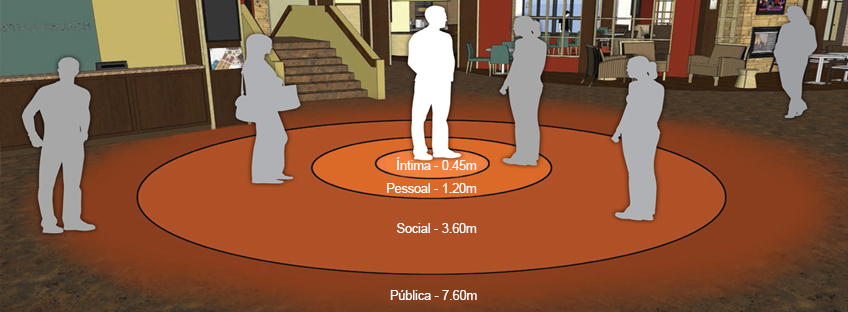
\includegraphics[width=\textwidth]{images/proxemicszones.png}
	\caption{Zonas de Proximidades definido por \citeonline{Argyle:1988}.}
	\label{fig:proximityzones}
\end{figure}

Cada uma das zonas de proximidades apresentadas na figura~\ref{fig:proximityzones} possui características particulares que pode guiar como ocorrerão as interações sociais. Na zona de proximidade social, o individuo pode emitir sons com um volume maior do que a zona de proximidade íntima que, por estarem muito próximos os indivíduos acabam se comunicando quase com sussurros. Interações na zona íntima são esperadas normalmente entre amigos muito próximos ou entre casais~\cite{Hall:1969, Argyle:1988}. O comportamento aceitável em zonas de proximidades mais distantes, como a social e a pública, é a comunicação com uma intensidade dos movimentos mais amplos e com uma força física maior que nas regiões mais próximas, onde há uma probabilidade maior de assustar o individuo com esse tipo de comportamento~\cite{Henkel:2014}.

Além dos comportamentos diferentes em cada zona de proximidade, existe um outro fator que pode atrapalhar a interação exclusiva entre duas pessoas nas regiões mais distantes. A existência de muitas pessoas ao redor das regiões mais distantes pode dificultar o estabelecimento uma interação exclusiva devido ao excesso de ruído no cenário. O ruído para esse cenário pode ser considerado através do volume excessivo de pessoas no local, junto com a altura dos sons emitidos e além da quantidade de gestos que cada individuo realiza simultaneamente~\cite{Walters:2009, Henkel:2014}.

Entretanto, não é apenas o espaço social que as \emph{Proxemics} se referem na análise comportamental. Algumas variáveis que são utilizadas para a leitura corporal também são utilizadas para a análise comportamental através das \emph{Proxemics}. \citeonline{Mead:2013} lista algumas variáveis consideradas em seu trabalho, além da distância social, são elas: (I) orientação da postura; (II) orientação do quadril; (III) orientação dos ombros; (IV) posicionamento e orientação da cabeça; e (V) fixação do olhar entre os indivíduos. Todas as variáveis apresentadas por~\citeonline{Mead:2013} auxiliam a determinar a qualidade da interação social entre dois indivíduos, agentes ou entre robôs e humanos.

\emph{Proxemics} tem sido explorado em trabalhos de interação humano-robô~(IHR) desde 1997, somando aproximadamente 25 trabalhos ao todo~\cite{Henkel:2014}. Assim, a próxima seção apresentará os trabalhos relacionados que abordam o tema da \emph{Proxemics} e as discussões sobre como eles auxiliam o trabalho apresentado nessa tese.

\section{\emph{Proxemics} e Interação Humano-Robô}
\label{sec:proxemicsihr}

Nessa seção são apresentados os trabalhos de \emph{Proxemics} aplicados a interação humano-robô~(IHR), como o trabalho de \citeonline{Walters:2009} que propõem um \emph{framework} empírico com o objetivo de auxiliar a detecção da distância real, ou seja, a distância considerando fatores diversos da IHR.

Alguns fatores de impacto na IHR foram apresentados por \citeonline{Walters:2009} na discussão de seu trabalho. Um dos fatores explorados foi o impacto dos sons emitidos pelo robô durante a interação, ou seja, a voz do robô. A voz não causa impacto apenas pelo volume que é emitida, mas também o estilo dela que pode influenciar uma vez que é possível inferir emoções a partir do estilo em que a voz é emitida. Além disso, a voz também pode influenciar no tempo de aproximação entre o robô e o individuo, pois dependendo de como o som é emitido pode gerar insegurança ao individuo que está interagindo com o robô~\cite{Walters:2009}.

Fatores como a aparência do robô e informações demográficas como idade, gênero, grau de instrução, personalidade, carisma, entre outros também podem interferir na IHR. Por exemplo, as pessoas preferem manter uma distância maior dos robôs que possuem uma aparência humanoide, pois ela causa um pouco de preocupação sobre as ações dele, quando comparado a um robô com aparência mais mecânica. Entretanto, a altura do robô não é um fator que apresenta grande relevância para IHR~\cite{Walters:2009}.

Outro trabalho, apresentado por \citeonline{Torta:2011}, tem como objetivo a apresentação de um arquitetura para robótica baseada em comportamento que permite ao robô navegar em segurança por um ambiente doméstico mutável e consiga codificar interações não verbais de maneira embarcada. Dessa maneira, é possível fazer com que o robô possa apresentar o comportamento de aproximação adequado ao seu objetivo, utilizando um novo modelo de espaço pessoal.

Esse novo modelo considera a relação entre a orientação do robô em conjunto com a distância do objetivo e ainda a avaliação do individuo para a orientação de aproximação do robô~\cite{Torta:2011}. Para alcançar esse objetivo \citeonline{Torta:2011} utilizaram um filtro Bayesiano para inferir a localização do objetivo a partir da posição do robô de maneira dinâmica. O filtro Bayesiano é utilizado como guia para o robô em seu algoritmo de navegação. 

Nos testes utilizou-se o robô NAO e obteve a validação de que a inclusão do espaço pessoal no algoritmo de navegação trouxe resultados positivos ao modelo implementado. Em estudos futuros, \citeonline{Torta:2011} incluirão outros fatores ao cenário de IHR, como a altura do robô, a aparência e o propósito da interação, e a partir dessas novas variáveis identificar como é possível melhorar a interação de tal forma, que esse modelo obtenha uma qualidade maior em sua aplicação~\cite{Torta:2011}.

A aplicação de \emph{Proxemics} não é exclusiva a robótica social ou doméstica, \citeonline{Srinivasan:2012} aplicam o conceito para o cenário de resgate de vítimas. O trabalho apresentado tem como objetivo avaliar a utilização do olhar social com movimentos de cabeça e funções escalares de \emph{Proxemics} para auxiliar na aproximação e trabalho em regaste de vítimas em centros urbanos.

Nesse cenário o robô deve manter a vítima calma, tranquila, com pensamentos positivos e cuidar dela, na medida do possível, até que o resgate consiga acesso ao local para que o trabalho de extração seja realizado com sucesso~\cite{Srinivasan:2012}. Dois cenários de simulação foram utilizados para validar o método proposto por \citeonline{Srinivasan:2012}. No primeiro cenário observou-se como a vítima correspondia a medida que o robô gesticulava com a cabeça durante a interação comparado ao robô totalmente estático. O movimento da cabeça foi programado para ficar sincronizado com a fala do robô de tal forma, que seu comportamento ficasse próximo a um comportamento natural. Neste primeiro cenário, foi validado a hipótese de que o usuário prefere o robô que tem o movimento social (gesticulação da cabeça) ao invés do robô que permanece totalmente estático durante a interação.

No segundo cenário de simulação, utilizou-se funções escalares para definir a aproximação do robô junto à vítima. Nessa aproximação são consideradas as quatro regiões de proximidades, apresentadas na figura~\ref{fig:proximityzones}, para determinar a interação com a vítima. Foram comparadas três tipos de funções: (I) Logarítmica; (II) Linear; (III) Não escalar. Nos testes os melhores resultados foram obtidos através da função logarítmica, seguida pela função linear e depois a função não escalar~\cite{Srinivasan:2012}. Dessa forma, \citeonline{Srinivasan:2012} esperam melhorar a abordagem com robôs à vítimas de desastres em cenários de centros urbanos.

\citeonline{Okita:2012} realizaram um estudo para identificar quais fatores mais auxiliam na redução da distância física entre o robô e o ser humano. Foram utilizados dois tipos de abordagem para os testes realizados: (I) Robô com a iniciativa de se aproximar do ser humano; e (II) Humano com a iniciativa de se aproximar do robô.

Para o teste de ambos cenários foram utilizados dois tipos de indivíduos, separados em dois grupos diferentes, crianças e adultos. Na execução do teste, \citeonline{Okita:2012} utilizaram o método chamado de \emph{Wizard of Oz} (WOZ) que permite operar o robô através de um controle remoto distante da vista do indivíduo em interação. Dessa forma, é possível passar a impressão de que o robô é autônomo e ao mesmo tempo ter o controle dele para que não ocorra nenhum acidente durante a interação.

O experimento foi executado de duas maneiras diferentes sendo uma o robô aproximar-se sem nenhum tipo de aviso prévio e a outra maneira era exatamente avisar sua aproximação. Observou-se que quando o robô solicitava a permissão para aproximar do individuo o resultado sempre era positivo para a interação, quando comparado à aproximação sem aviso ou com aviso posterior a ação do robô~\cite{Okita:2012}.

Muitos trabalhos apontam maneiras de aplicar o estudo de \emph{Proxemics} em interações sociais. Algumas variáveis que podem afetar a interação são funções interpessoais de relacionamento, fatores fisiológicos moldados pela cultura de origem de um indivíduo, perspectivas etnológicas, além de informações sobre o ambiente de interação, como a luz ambiente, localização e ocupação física do agente, tamanho, entre outros fatores~\cite{Mead:2011b}.

Com a facilidade de compra dos sensores de captura de movimento não invasivo como o Microsoft\textregistered\ Kinect\textregistered ou o PrimeSensor\textregistered, os pesquisadores \citeonline{Mead:2011b} apresentam em seu trabalho um conjunto de métricas que são capazes de auxiliar na automatização do processo de análise do comportamento para distância social. As métricas por eles estabelecidas são: postura, posição do quadril, do ombro, do torso, dos braços, distâncias entre os agentes, gênero, entre outros.

Com base nas métricas definidas foi realizado um estudo conceitual para verificar se o cenário com um Kinect\textregistered\ inserido no ambiente, fosse capaz de capturar todas essas informações para que a partir delas torna-se possível a criação de um mecanismo de análise automática do comportamento de agentes em um ambiente de interação social. Os testes preliminares ocorreram conforme o esperado, possibilitando a validação do cenário apresentado por \citeonline{Mead:2011b}.

Um cenário e ferramenta para coleta de informações sobre indivíduos em interação social são apresentados também por \citeonline{Mead:2011}. O principal objetivo é utilizar as informações coletadas em estudos futuros. Essas informações serviram para a criação de um modelo oculto de Markov (\emph{Hidden Markov Model} (HMM), em inglês) com seis classes para auxiliar na predição das \emph{Proxemics} de interação face a face. Nesse estudo, o HMM demonstrou-se com um desempenho superior para a tarefa de predição, quando comparado com um classificador aleatório ponderado por pesos~\cite{Mead:2011}.

\citeonline{Mead:2012} apresenta uma discussão sobre os tipos de representações para \emph{Proxemics}. Essas representações são: física e psicológica. Além desses dois tipos é proposto uma representação psicofísica que apresenta uma abordagem permitindo unir melhor as qualidades dos outros dois tipos de representação. A representação física tem como objetivo analisar como o espaço social é ocupado por dois indivíduos e é a abordagem mais comum em estudos de \emph{Proxemics}, tanto para interações humano-humano quanto para interações humano-robô. A representação psicológica mantém o foco em fatores de relacionamento interpessoal de alto nível entre dois ou mais indivíduos. Esse fatores estão relacionados a teoria de conflito afiliativo~\cite{Argyle:1965} e também a teoria de adaptação interpessoal~\cite{Burgoon:2007}. 

Porém, com as lacunas existentes nesses dois tipos de representação de \emph{Proxemics}, foi proposto o tipo psicofísico. Esse tipo de representação tem como objetivo principal analisar a percepção e a produção de estímulo social entre dois ou mais indivíduos interagindo. A abordagem psicofísica é discutida também por~\citeonline{Hall:1969}. Essa representação está diretamente ligada com a experiência sensorial do estímulo social até os parâmetros espaciais de maneira física. A partir da representação psicofísica é realizado um estudo para capturar informações que servirão de base para treinamento de dois HMM. Cada HMM é responsável por uma exclusiva tarefa, início da interação ou término da interação. Essa representação deve auxiliar nas pesquisas de interação humano-robô, no intuito de que seja possível realizar uma análise para a interação ocorrer com maior qualidade~\cite{Mead:2012}.

Outro trabalho de \citeonline{Mead:2012b} apresenta um mecanismo de análise comportamental através da \emph{Proxemics}. Utiliza-se modelos probabilísticos de tal forma, que seja possível determinar alguns comportamentos dos indivíduos durante uma interação. Como métrica de proximidade utilizou-se a estratégia do mundo de grades para predizer a distância aproximada entre o robô e o individuo. Esse trabalho é implementado através de uma rede Bayesiana dinâmica como uma melhora para o mecanismo~\cite{Mead:2012b}.

Conforme tem sido discutido ao longo dessa seção, para que a interação entre um humano e um robô possa ocorrer de maneira confortável e com qualidade, é necessário que o robô entenda as variáveis de espaço social. Além disso, é necessário também que ele possua o controle sobre essas variáveis de tal forma, que ele consiga tomar decisões sobre as ações que executará~\cite{Mead:2013b}.

\citeonline{Mead:2013b} apresentam um estudo baseado principalmente com variáveis de voz e gestos, utilizando um método de amostragem que tem como entrada a postura do indivíduo ao interagir com o robô. A maior contribuição esperada por \citeonline{Mead:2013b} é a apresentação do entendimento obtido através das interações pré culturais que estão inseridas junto ao estudo de \emph{Proxemics}. O resultado apresentado é apenas uma base de dados para investigar todos os aspectos da interação humano-robô apresentadas no trabalho (voz e gestos).

A partir da base de dados gerada por \citeonline{Mead:2013b}, é apresentado outro trabalho onde \citeonline{Mead:2013} discutem a utilização de um HMM para extração de características comportamentais espaciais do ser humano, em outras palavras, \emph{Proxemics}. Alguns fabricantes de sensores de movimentos, como o Microsoft\textregistered\ Kinect\textregistered\ e o ASUS\textregistered\ Xtion, têm pesquisado técnicas para aprimorar o estudo das distâncias sociais e também seus significados.

Com base nesses estudos, \citeonline{Mead:2013} analisam a possibilidade de automatizar o processo de análise das \emph{Proxemics}. A intenção do trabalho é extrair variáveis para que seja, então, possível determinar o início e o fim de uma interação social através de um HMM. Para realizar os experimentos foram necessários dois indivíduos e um robô aplicados a um cenário de interação, onde os indivíduos se aproximam do robô sendo que os indíviduos estão separados por uma parede. Os resultados são apresentados em relação ao ponto de vista físico e psicológico. Na detecção das variáveis que representam as \emph{Proxemics} de maneira dinâmica, \citeonline{Mead:2013} consideram os resultados satisfatórios e como sequência do trabalho é mantido o foco em interações com fatores psicológicos complexos, para aprimorar a precisão do \emph{framework} criado.

\citeonline{Mead:2014} direcionam o foco de seu trabalho para a análise de conversa social e gestos, tanto na questão de produção das conversas e gestos de maneira automática quanto para o reconhecimento, aplicados em interações humano-humano e humano-robô. Todo o trabalho realizado está relacionado com o estudo de \emph{Proxemics} na interações sociais, uma vez que essas tem o objetivo de não só identificar as variáveis, mas também de interpretar, manipular e compreender a dinâmica do comportamento espacial dentro do cenário das interações sociais.

Os estudos e experimentos sociais realizados por \citeonline{Mead:2014} auxiliaram na coleta de informações sobre o volume da fala de acordo com a distância, além dos gestos que necessitam de espaços maiores para execução sem prejudicar a interação. Os resultados apresentados apontam que a distância de interações entre humanos é menor que a distância da interação entre um humano e um robô. Além disso, os resultados obtidos não são aplicados à múltiplas culturas (nesse caso origem dos indivíduos), e isso deve ser realizado em outros trabalhos segundo \citeonline{Mead:2014}. Um mecanismo para personalizar o tratamento que o robô terá com o indivíduo durante a interação também é algo de deve ser construído ao longo dos trabalhos futuros.

Analisando a diferença de cultura para variáveis de \emph{Proxemics}, \citeonline{Eresha:2013} apresentam como objetivo do trabalho a avaliação do comportamento de indivíduos ao se encontrarem com dois robôs interagindo entre si e caminhando em direção ao individuo de tal forma que este possa também interagir ou não com os robôs conforme se aproximam. Além de avaliar o comportamento dos indivíduos durante a interação com os robôs, \citeonline{Eresha:2013} adicionaram a variável de cultura ao estudo. O objetivo é identificar como é a diferença de comportamento entre culturas diferentes. Foram escolhidos participantes de origem árabe e alemã para o estudo.

Nos experimentos, \citeonline{Eresha:2013} utilizaram dois robôs NAO que se posicionavam a 40 cm de distância entre eles e caminhavam até ficarem a uma distância diagonal de 85 cm do indivíduo. Para o experimento houve a participação de 24 indivíduos, 12 árabes e 12 alemães, sendo metade do gênero feminino e a outra metade do gênero masculino. Os testes apresentaram resultados interessantes, pois alguns indivíduos não reagiram como o esperado para pessoas de sua origem e muitas vezes o comportamento social na interação era idêntico entre alemães e árabes. Outro ponto apresentado por \citeonline{Eresha:2013} é que durante os testes dois alemães apresentaram o sentimento de medo de serem atacados fisicamente pelos robôs.

O trabalho de \citeonline{Eresha:2013} apresenta indícios de que as variáveis de \emph{Proxemics} não estão ligadas a cultura do indivíduo, como origem, mas sim na experiência cultural que este teve ao longo de sua vida. Dessa maneira, pode-se dizer que \emph{Proxemics} são variáveis extraculturais, porém é necessário realizar um tratamento para esse tipo de condição de tal forma, que o robô possa interagir com mais qualidade com pessoas que possuem diferentes experiências culturais.

\citeonline{Henkel:2012} investigam características entre diversas plataformas de teste para interação humano-robô, e com base no resultado deste estudo é realizado a proposta de uma nova plataforma de testes. A nova plataforma foi desenvolvida, pois \citeonline{Henkel:2012} alegam que não existe nenhuma plataforma de teste capaz de atender aos seis atributos de dependência das \emph{Proxemics}. Os atributos são: (I) movimento afetivo; (II) leitura das \emph{Proxemics}; (III) interação de voz; (IV) manipulação do estilo de áudio; (V) controle do olhar; e (VI) apresentação de conteúdo através de mídia, por exemplo, monitor ou leds.

A plataforma é constituída por uma cabeça feita com um monitor de 7'', junto com um encaixe construído para ser acoplado em qualquer base de robôs já existentes no mercado. Alguns testes que foram realizados no cenário de resgate à vítimas demonstram que as pessoas que tinham a zona de espaço social íntimo invadida por qualquer parte do robô sem uma interação prévia ficavam em situação de \emph{stress} elevado. Essa reação foi totalmente oposta quando o robô iniciava com qualquer tipo de interação antes de realizar a aproximação do indivíduo~\cite{Henkel:2012}. O primeiro contato antes da aproximação para uma interação maior é importante, pois esse comportamento pode definir o quão confortável a interação entre os agentes será e esse comportamento deve ser explorado durante a execução dessa tese. 

Em outro trabalho, \citeonline{Henkel:2014} apresentam duas funções escalares para avaliar os valores de proximidade entre humanos e robôs. As funções escalares são comparadas com outras funções não-escalares e também entre si de tal forma, que seja possível uma tomada de decisão em tempo de execução da ação/interação. As duas funções escalares apresentadas são: (I) logarítmica; e (II) linear.

Os testes foram executados no cenário de regaste à vitimas. Quando a função logarítmica foi aplicada, os resultados apresentados foram melhores do que os obtidos com as demais funções. Como o principal objetivo de \citeonline{Henkel:2014} é generalizar o método para outros cenários, eles pretendem realizar testes do modelo em outras situações e também utilizando outros tipos de robôs para sustentar melhor a hipótese. Os estudos prévios realizados demonstram que a generalização do modelo é possível.

A integração social do robô com os ambientes que envolvem cenários de cuidados médicos, construção, educação, serviço públicos, entre outros pode ser a chave de sua aceitação por parte dos seres humanos. Um dos caminhos para conseguir esse objetivo é fazer com que o robô saiba ter um comportamento adequado de interação em cada um desses cenários, assim como o que já é demonstrado em filmes de ficção científica. Dessa maneira, é possível fazer com que os seres humanos utilizem o próprio senso social para identificar essas habilidades no robô, quebrando um pouco o medo de interagir com ele~\cite{Heenan:2014}.

Como primeiro passo para que a interação ocorra naturalmente entre o ser humano e o robô, \citeonline{Heenan:2014} acreditam que deve haver sempre uma saudação entre ambas partes logo ao primeiro contato. Esse tipo de comportamento pode ser fundamental para que haja uma aceitação social do robô entre as pessoas. Durante uma saudação existem diversos fatores que são analisados implicitamente pelo ser humano, como nuanças de comunicação não verbal, vocalização das palavras e a distância inter pessoal. Esses fatores devem ser considerados ao projetar uma saudação por parte do robô, fazendo com que seja possível o robô iniciar a interação.

Fazer com que um robô realize uma saudação natural não é uma tarefa muito fácil. Deve ser considerado que um robô não tem a mesma capacidade de identificar as nuanças sociais com a mesma velocidade de um ser humano. Outro ponto negativo é que o robô possui o lado mecânico limitado, quando comparado a musculatura do ser humano. Assim, o primeiro objetivo do trabalho de \citeonline{Heenan:2014} é definir um subconjunto exato de elementos de uma saudação social que possa ser articulado pelo robô durante a tarefa e ainda como implementar as sutilezas do comportamento da interação de saudação social.

Os testes executados demonstram que a saudação é um ponto importante para o resultado com sucesso da interação com o ser humano. O robô NAO utilizado nos testes foi capaz de implementar ações de comportamento como o contato visual, linguagem corporal e distância social para comunicação efetiva. Apesar de algumas restrições do modelo de saudação ocorrerem devido a limitação do NAO, é possível realizar a generalização do mesmo para outros robôs~\cite{Heenan:2014}.

Percebeu-se que o contato visual se apresentou como um elemento de interação social bem natural, contudo deve-se tomar cuidado para que o robô não fique encarando a pessoa constantemente, pois é gerado um desconforto para a pessoa durante o contato. \citeonline{Heenan:2014} dizem que é possível afirmar que utilizar a saudação é importante no primeiro contato de dois agentes, além de aumentar a capacidade da interação social entre o robô e o ser humano.

\citeonline{Vazquez:2014} apresentam um robô móvel no formato de mobília, chamado Chester, construído para realizar interações com crianças. Como o Chester é muito grande optou-se por usar um segundo robô não móvel, ao qual \citeonline{Vazquez:2014} denominam \emph{sidekick}. O \emph{sidekick} é como um parceiro ou personagem secundário que auxilia as pessoas em volta a prestarem atenção no personagem principal, como por exemplo o burro da animação Shrek. O \emph{sidekick} criado é um abajur chamado Blink. Ele fica acoplado em cima do Chester. A figura~\ref{fig:vazquez} apresenta a combinação dos robôs Chester e Blink.

\begin{figure}[ht!]
	\centering
	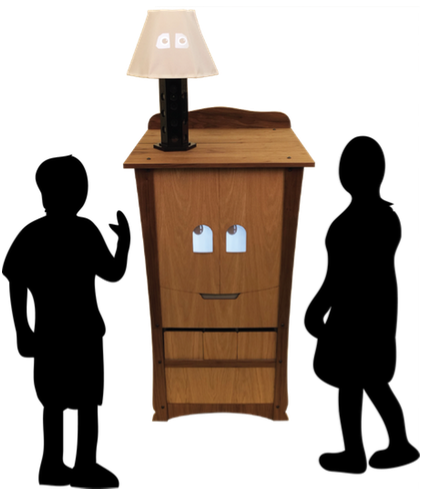
\includegraphics[width=0.4\textwidth]{images/vazquez2014.png}
	\caption{Chester e Blink os robôs apresentados por \citeonline{Vazquez:2014}.}
	\label{fig:vazquez}
\end{figure}

Blink tem uma linguagem própria e apenas o Chester é capaz de entender. É como o R2D2 em Star Wars que apenas alguns personagens são capazes de compreende-lo e falar com ele diretamente. Os resultados obtidos mostram que a inserção de um \emph{sidekick} não altera a questão de proximidade das crianças em relação ao robô, mas melhora a atenção com os elementos falantes do cenário~\cite{Vazquez:2014}.

Foi possível caracterizar alguns comportamentos das crianças ao interagir com os robôs. É afirmado por \citeonline{Vazquez:2014} que o formato de mobília para robôs é plausível para utilizar em robôs que interagem com crianças, pois elas se sentem mais empáticas aos robôs. Contudo, é questionável essa afirmação. Será que o que realmente influenciou esse resultado foi o formato do robô ou foi seu comportamento durante o contato com as crianças? Provavelmente, esse é um resultado que pode ser obtido com a mistura desses dois fatores, aparência e comportamento.

Por questões de segurança os testes foram executados utilizando o método \emph{Wizard of Oz} (WoZ), onde existe um especialista controlando o robô através de um controle de videogame, por exemplo. Foram conduzidos duas variantes do teste, são elas: (I) com o \emph{sidekick} ativo; e (II) com o \emph{sidekick} inativo. O especialista que controla o robô encontrava-se na mesma sala de teste, mas algumas precauções foram consideradas para que não houvesse ruído nos resultados do teste. Uma dessas precauções foi inseri-lo na sala do teste antes do mesmo iniciar para que aparenta-se que ele estava apenas trabalhando normalmente. Além disso, o controle do robô foi posicionado embaixo da mesa para facilitar a oclusão do objeto e ainda fez com que nenhuma criança notasse que o robô era teleoperado por um especialista~\cite{Vazquez:2014}.

Para capturar as informações de distância foi acoplado ao teto um sensor Microsoft Kinect. Ele é responsável por capturar as informações de distância entre o robô e a criança interagindo com ele. Notou-se que na maioria das vezes a criança ficava sempre de frente a face do robô e não ao seu lado ou atrás dele. Variáveis como o tempo de resposta para se afastar enquanto o robô dizia ``recue'' também foi considerado para identificar os resultados~\cite{Vazquez:2014}.

Nos resultados finais, \citeonline{Vazquez:2014} encontraram algumas limitações do robô e também do experimento, como por exemplo, o pouco conteúdo de linguagem que o robô possui implementado para dar respostas aos participantes do teste. Outro problema encontrado foi no início e no final de interação onde outros pontos do cenário e tarefa atrapalharam a coleta de informações ou melhor o foco do caso de estudo. Devido a esse problema, a utilização de um \emph{sidekick} deverá ser estuda com mais detalhes e realizar os testes novamente para que possa ser comprovado o real benefício dele nos resultados da interação. Resultados preliminares confirmam que o \emph{sidekick} não atrapalha na interação entre o robô principal e as pessoas e ainda auxilia a aumentar a atenção das pessoas o que auxilia em um melhor comportamento reativo dos participantes~\cite{Vazquez:2014}.

Alguns estudos utilizando robôs para interagir com crianças com autismo apontam que pode apresentar reações positivas e negativas para o âmbito social. Especialistas são capazes de identificar esse tipo de avaliação através da análise dos vídeos gravados entre sessões. O objetivo do trabalho de \citeonline{Feil-Seifer:2010} é automatizar esse processo de análise através do uso de robôs. Para isso foi desenvolvido um classificador heurístico para discretizar as crianças que conseguem interagir com o robô daquelas que não conseguem.

O cenário de teste é composto de uma sala, um robô totalmente autônomo com o objetivo de incentivar a interação, uma criança diagnosticada com autismo e um familiar mais próximo. Para incentivar a interação o robô deve se aproximar apresentando vocalizações de sons felizes e também esboçar um sorriso para a criança, por exemplo. Caso alguma criança se afaste do robô, ele deve esboçar uma face triste e emitir sons que demonstre a sua não felicidade~\cite{Feil-Seifer:2010}.

Durante os testes foram gravados vídeos e algumas marcações foram realizadas no robô, e nos pais, com o intuito de auxiliar na medida das distâncias entre a criança e o robô ou seus pais. Para realizar uma avaliação sobre esse cenário foi utilizada a seguinte heurística: Para cada trecho de tempo se a criança encontrar-se a 0,85 m dos pais ela é considerada próxima à eles. Caso ela encontra-se a 0,5 m de uma parede ela é considerada próxima a parede. Para ser considerada atrás do robô ela deveria estar a qualquer distância, mas entre uma angulação maior que 135º e menor que -135º~\cite{Feil-Seifer:2010}.

A partir das informações capturadas é possível gerar o classificador onde ele análise se pelo menos 50\% do tempo gasto é com as informações de comportamento negativo (mapeado pelas heurísticas), então é considerado que a criança não deseja interagir com o robô. Caso contrário, menos de 50\% do tempo gasto, a criança deseja interagir com o robô. Apesar dos resultados positivos, esse classificador não deve ser considerado como regra para que haja uma maior escalabilidade do projeto e sua aplicação~\cite{Feil-Seifer:2010}. Esses tipos de parâmetros podem auxiliar na determinação de interação ou não interação. Dessa forma, pode-se fazer com que o robô recue ou tente uma nova abordagem, para quando a reação do indivíduo for negativa.

Outros estudos confirmam a existência de uma relação de distância social entre o robô e o ser humano, entretanto nenhum método foi proposto computacionalmente para que haja uma geração do comportamento em relação a essa distância~\cite{Henkel:2012b}. Assim, é apresentado um método escalar do comportamento do robô de tal forma, que esse comportamento baseado na distância social tenha como suporte uma lei física e duas psicológicas: \emph{inverse-square law}, \emph{Weber-Fechner law} e \emph{Steven's Power law}~\cite{Henkel:2012b}.

O cenário de teste é um ambiente de desastre no qual o robô deve localizar a vítima. A interação ocorre por meio de voz sintetizada, caminhos pre definidos e controle segundo o módulo de teste WoZ. Como meio de avaliação questionários pré e pós interação são aplicados aos usuários que participam do teste~\cite{Henkel:2012b}.

Atributos primários foram determinados para que possam ser identificados alguns níveis de consistências sociais: conforto, movimentos naturais, consideração do espaço pessoal, segurança e controle próprio. Atributos secundários também foram considerados nos estudos de \citeonline{Henkel:2012b}, são eles: atenciosidade, empatia, felicidade, similaridade, inteligência, sensibilidade, submissão e confiança. Os resultados demonstram que todos atributos primários e apenas três secundários provaram que apresentam melhor significância para o processo. O sistema de percepção escalar provou ser melhor do que o não escalar. O modelo escalar linear apresentou o mesmo resultado que o não escalar~\cite{Henkel:2012b}.

\citeonline{Hemmert:2013} apresentam um trabalho que tem como objetivo a aplicação dessa técnica em aparelhos de telefonia móvel. A ideia principal é fazer com que o telefone reaja de acordo com a aproximação do aparelho pela voz da pessoa. O foco principal dentre as oito variáveis de \emph{Proxemics} é a postura do usuário. Interações de \emph{Proxemics} tem sido um dos modelos gerais em interação humano-computador (IHC). Entretanto, é um tema pouco explorado em telefonia móvel~\cite{Hemmert:2013}.

O projeto utilizado no caso de estudo apresenta uma nova maneira de interagir com dispositivos móveis, em especial telefones, tendo como base variáveis de linguagem corporal e proximidade do indivíduo para com o aparelho. Como trabalho futuro \citeonline{Hemmert:2013} querem apresentar um modelo que faça a leitura de diversas variáveis com o intuito de entender por completo como elas funcionam no comportamento do ser humano.

Um ponto interessante abordado por \citeonline{Hemmert:2013} é quando ele faz refêrencia ao uso de \emph{Proxemics} em IHR. Geralmente os trabalhos de \emph{Proxemics} são voltados ao comportamento de ser humano, e nenhum possui foco na reação do robô, ou seja, como esse robô reagirá caso um ser humano invada o espaço íntimo do robô sem consentimento. Esse é um ponto interessante que deve ser explorado ao longo dessa tese. 

Outro ponto chave dos trabalhos apresentados ao longo dessa seção é que sempre utilizam sensores no ambiente para medir as variáveis de \emph{Proxemics} entre a pessoa e o robô. Contudo, acredita-se que esse tipo de abordagem não é natural ao robô móvel, pois os seres humanos não tem o auxílio sendo assim o robô também não deve utilizar desses recursos. Contudo, as variáveis de \emph{Proxemics} se mostram essenciais para determinar o sucesso de uma interação ou não, e devem ser consideradas ao longo da proposta desta tese de doutorado.

Dessa forma, todas as variáveis apresentadas nos trabalhos dessa seção são importantes para avaliar o comportamneto de um indivíduo durante uma interação com robôs e até outros dispositivos tecnológicos. Na seção~\ref{sec:extracaocaracteristicas} são apresentados as variáveis consideradas para o desenvolvimento desse trabalho. Além das variáveis, também são avaliados os meios de captura das informações visando a aplicação do trabalho desenvolvido na tese inserido em um ambiente inteligente.
%!TEX root=Principal.tex
\chapter{CONCEITOS FUNDAMENTAIS}
\label{cap:ai}
Este capítulo apresenta os conceitos fundamentais das técnicas utilizadas para desenvolvimento da tese apresentada.

\section{Agrupamento de Dados}
\label{sec:clustering}
Encontrar padrões em informações do mundo real é uma tarefa complexa. O conhecimento sobre o domínio de aplicação ou dos fenômenos naturais é imprescindível na maioria dos casos. Sem esse conhecimento, gerar modelos e padrões matemáticos para compreender os efeitos de tal fenômeno ou aplicação no mundo é complicado~\cite{kantardzic:2011}.

Com o avanço da tecnologia e sua popularização ocorreu um aumneto na criação de informações, sendo este sem ordem ou normalização. O mundo coorporativo enxergou nesse fenômeno uma potencial fonte de conhecimento. Porém, encontrar padrões ou modelos que torne possível encontrar conhecimento nessas informações não é uma tarefa trivial. A partir desse problema, pesquisadores começaram a desenvolver técnicas e algoritmos computacionais onde houvesse então a mineração dos dados, como ficou conhecida a técnica~\cite{jain:1999, kantardzic:2011}.

Minerar dados é um processo realizado com dois objetivos. Predição da informação, onde é possível prever o futuro com base em algumas informações coletadas. E descrição da informação, que apresenta um rótulo mais compreensível ao ser humano a partir dos padrões encontrados nos dados coletados~\cite{jain:1999}.

Dentro do processo de mineração de dados existe um passo chamado de agrupamento de dados. O agrupamento de dados é fundamental para, a partir de um volume finito de informação, extrair padrões e forma grupos com base na similaridade encontrada em cada registro. A extração dos padrões tem como base algumas técnicas aplicadas para associação e classificação. O resultado final dos padrões encontrados pode variar dependendo das técnicas aplicadas~\cite{kantardzic:2011, witten:2011}. As técnicas existentes são:

\begin{itemize}
    \item \textbf{Exclusivo}: os elementos pertencem a um grupo apenas;
    \item \textbf{\emph{Overlaping}}: os elementos podem pertencer a mais de um grupo, simultâneamente;
    \item \textbf{Probabilístico}: os elementos possuem um grau probabilidade de pertencer a um grupo;
    \item \textbf{Hierárquico}: realiza a divisão aproximada dos grupos. Refina a divisão encontrada até que alcance um resultado que não se altere muito entre as iterações.
\end{itemize}

O maior desafio da técnica de agrupamento de dados é a maneira de tratar e associar os diversos tipos de informação existentes com por exemplo, algarismos, textos e imagens. Além disso, as informações podem ser extraídas de maneira qualitativa ou quantitativa~\cite{witten:2011}. A seção~\ref{sec:algoritmosclustering} apresentará alguns dos principais algoritmos de agrupamento de dados existentes.

\subsection{Algoritmos de Agrupamento de Dados}
\label{sec:algoritmosclustering}
Para realizar o agrupamento de informações existem diversos algoritmos. Alguns dos algoritmos mais populares e outros com aplicações mais específicas serão apresentados nessa seção.

Dentre os algoritmos existentes o mais popular é o k-means. Ele utiliza da distância eucliana para comparar a similaridade entre os dados, tentando minimizar o erro quadrático. A partir do momento que o erro não tiver mais alterações entre as iterações do algoritmo, ele encerra o processo de agrupamento. Ele precisa que o número de grupos desejados seja informado e realiza uma inicialização de sementes, para cada grupo, de maneira aleatória. Devido a isso, o resultado do agrupamento pode ser diferente entre as execuções do algoritmo. O resultado do k-means é bem consistente, mas mesmo para apenas dois grupos, encontrar a solução ótima com o k-means é um processo considerado NP-\emph{Hard}~\cite{jain:2010, witten:2011}.

\emph{Graph-based Clustering} (GBC) é um algoritmo de agrupamento baseado na teoria de grafos. Ele liga uma aresta entre os dados e o ponto médio entre as arestas é utilizado para determinar a divisão dos grupos de maneira automática. O problema apresentado pelo GBC é na concentração densa dos dados. Quando ocorre esse tipo de cenário, o algoritmo acaba considerando todos os dados pertencentes a um único grupo~\cite{muhlenbach:2009}.

Outro algoritmo existente é o \emph{Quick ROCK} (QROCK) que tem como objetivo o agrupamento de informações categóricas, ou seja, informações textuais. Ele é um algoritmo de agrupamento hierárquico aglomerativo. Assim como o GBC ele determina o resultado com base na conexão dos elementos através de um grafo. Para determinar a quantidade de grupos é necessário informar um valor de corte $\theta$ representando o valor de similiaridade entre os dados. Esse valor é calculado com base na equação~\ref{eq:sim_qrock} e tende a deixar o agrupamento mais natural~\cite{dutta:2005}.

\begin{equation}
    \label{eq:sim_qrock}
    SIM(X, Y) = \frac{X \bigcap Y}{X \bigcup Y}
\end{equation}

Com o foco em agrupamento de informações espaciais, o algoritmo \emph{Density Based Spacial Clustering of Applications with Noise} (DBSCAN) foi apresentado por~\citeonline{ester:1996}. Para realizar o processo de agrupamento, são necessários dois parâmetros. Distância mínima entre dois pontos, que auxilia ao dizer se os pontos fazem parte ou não do mesmo grupo. E o outro parâmetro é a quantidade mínima de pontos para formar um grupo. Esse último parâmetro é importante para determinar se existirá um grupo ou se alguns pontos serão considerados como ruídos e desconsiderados do resultado final. Com base de dados espaciais em duas dimensões o DBSCAN conseguiu segmentar bem as diferentes regiões existentes, porém com dados de dimensões maiores isso já não foi possível.

\emph{Affinity Propagation} é um algoritmo de agrupamento sem necessidade de informar qualquer parâmetro para o processo. Ele considera todos os dados como potenciais centróides de grupos. E como uma rede neural de aprendizado competitivo, vai identificando os dados que possuem mais arestas e determinando os grupos com base nestes. Seu desempenho é considerado bom apenas quando o resultado inicial está próximo do ótimo~\cite{frey:2007}.

Perfis de usuários são compostos de diversos tipos de informação. Isso torna o processo de agrupamento mais complexo, pois é necessário criar uma regra de similaridade que atenda cada tipo de informação e também consiga estipular um valor único por perfil. Com esse problema em mente o algoritmo \emph{Quality Groups of Similarity Clustering} (QG-SIM) foi criado. É necessário informar o valor $q$ que representa a similaridade mínima para manter entre os elementos do grupo. Apesar de ser útil em diversas aplicações, o enfoque dele é em aplicações de perfis de usuários. Um ponto fraco dele é o desempenho computacional que depende da quantidade de dados dentro de cada um dos grupos~\cite{masiero:2013}.

A tabela~\ref{tab:comp_algo_agrupamento} apresenta uma comparação entre os algoritmos de agrupamento de dados e suas principais características.

\begin{table}[h!]
	\caption{Tabela comparativa entre os algoritmos}
	\label{tab:comp_algo_agrupamento}
	\begin{tabular}{ m{2.8cm} | m{5cm} | m{7cm} } \hline
	Categoria & Algoritmo & Parâmetro / Propriedades \\ \hline
	\emph{clustering} hierárquico & Ward & algoritmo aglomerativo \\ \hline
	& MST Divisivo & baseado na teoria de grafos \\ \hline
	& \emph{Clustering Using REpresentatives (CURE)} & cada grupo é representado por um conjunto de representações \\ \hline
	& \emph{RObust Clustering using linKs (ROCK)} & $k*$: número de grupos \\ \hline
	& QROCK (\emph{Quick} ROCK) & $\theta$: \emph{threshold} de similaridade  \\ \hline
	\emph{hard clustering} & $k$\emph{means} & $k*$: número de grupos \\ \hline
    & QG-SIM & $q$: similaridade mínima entre os elementos do grupo \\ \hline
	\emph{clustering} baseado em densidade & DBSCAN & $\epsilon$: distância para considerar se 2 pontos são ou não vizinhos \\ \hline
	& \emph{Affinity Propagation} & $\theta$: \emph{threshold} de similaridade  \\ \hline
	\emph{clustering} sequencial & \emph{Basic Sequential Algorithm Scheme (BSAS)} & $\Theta$: \emph{threshold} de não similaridade e $k*$: número máximo de grupos  \\ \hline
	\end{tabular}
	\smallcaption{Fonte: Adaptada de \citeonline{muhlenbach:2009}.}
\end{table}

Nesta tese, como há um trabalho de agrupamento de perfil de usuário, optou-se por utilizar o algoritmo QG-SIM que foi, de acordo com a literatura, o que apresentou melhores resultados para esse tipo de informação~\cite{masiero:2013}.

\section{Raciocínio Probabilístico}
\label{sec:raciocinio-probabilistico}
Para que um agente possa tomar uma decisão, é necessário que ele analise todas as possibilidades de ações que possam ser feitas e o que ocorrerá após essa tomada de decisão para que exista uma certeza sobre o caminho que ele deve seguir. O processo para encontrar a certeza sobre uma decisão, computacionalmente, é oneroso e com a quantidade de variáveis geralmente consideradas, torna-se inviável. Sendo assim, um agente precisa trabalhar com a incerteza sobre o domínio para que possa ser tomada uma decisão~\cite{russell:2002}.

Fazer o agente tomar uma decisão considerando a incerteza, é fazer o agente manter o controle baseado em um estado de crença, em outras palavras, um conjunto com todos os possíveis estados em um domínio ao qual ele possa estar. Além disso, o agente deve prever e gerar um plano de contingência para eventuais situações que sejam detectadas durante a execução do algoritmo. Nesses problemas, as informações que o agente possui não conseguem garantir nenhum resultado com certeza absoluta. Porém, tais informações garantem um grau de crença de que o objetivo será alcançado ou a decisão por um caminho relevante será tomada~\cite{russell:2002, faceli:2011}.

Todas as declarações feitas com base na crença sobre as informações não se contradizem mutuamente. Cada uma é uma afirmação separada de um diferente estado de conhecimento. Cada vez que inserimos uma informação nova e complementar, é aumentado o estado de crença sobre um determinado assunto, melhorando a tomada de decisão do agente~\cite{faceli:2011}.

Para que a tomada de decisão tenha uma maior utilidade para o agente, ele deve preferências dentre os diferentes resultados apresentados. Sendo assim, ter uma decisão com base apenas na probabilidade, não é recomendável. Essa é a base da teoria da utilidade. A teoria da utilidade é utilizada para que o agente represente e raciocine em seu problema, de acordo com suas preferências. É distribuido um grau de utilidade para cada escolha que o agente possa ter, assim o estado que possui o maior grau de utilidade é escolhido. Pode-se dizer então que uma decisão é tomada com base na probabilidade de um estado somado a sua utilidade~\cite{russell:2002}.

Utilizar as teorias de probabilidade e utilidade, necessita de algumas formalizações e notações, para que as equações sejam melhor compreendidas. A primeira formalização é a equação~\ref{eq:prob_condicional_a_b} que representa a probabilidade condicional para quaisquer proposições $A$ e $B$~\cite{russell:2002}.

\begin{equation}
    \label{eq:prob_condicional_a_b}
    P(a|b) = \frac{P(a \land b)}{P(b)}
\end{equation}

A equação~\ref{eq:prob_condicional_a_b} é válida apenas para $P(b) > 0$. Essa equação também pode ser escrita no formato de produto, conforme apresentado na equação~\ref{eq:prob_condicional_a_b_2}.

\begin{equation}
    \label{eq:prob_condicional_a_b_2}
    P(a \land b) = P(a|b)P(b)
\end{equation}

As proposições de uma equação são determinadas pelas variáveis aleatórias de um problema. Uma variável aleatória é representada através de um nome ao qual sua primeira letra deve ser maiuscula, por exemplo, $Total$, $Tempo$ ou $Informacao$. Cada variável aleatória possui um domínio, que representa os possíveis valores que esta variável pode assumir. Os valores são descritos utilizando todas as letras em caixa baixa, ou seja, minusculas, por exemplo, $Tempo = \{ ensolarado, chuvoso, nublado, nevando \}$. Quando uma variável é booleana, podem ser nomeadas com se fossem valores (em minusculo) e utiliza-se a regra de negar o valor para representar os valores de falso e verdadeiro~\cite{russell:2002}.

O exemplo da representação de uma varíavel booleana através de valores é demonstrado através das equações~\ref{eq:neg_valor}.

\begin{subequations}
    \label{eq:neg_valor}
    \begin{align}
        A = verdadeiro \rightarrow a\\
        A = falso \rightarrow \neg a
    \end{align}
\end{subequations}

Em teoria de probabilidade, quando trata-se um problema, é procurado mundos possíveis. Um mundo possível é definido como uma atribuição de valores para cada uma das variáveis aleatórias consideradas em um problema. Para realizar a atribuição dos valores, pode-se trabalhar com diversos tipos de visão probabilística. A primeira é chamada de frequentista, onde o valor da probabilidade é determinado através de observações à experimentos realizados com grandes amostras. Outro tipo encontrado é o objetivista que define as probabilidades como aspectos reais, ou seja, como tendências dos comportamentos dos objetos dentro de um cenário específico~\cite{russell:2002, faceli:2011}.

A visão subjetivista trabalha com os valores de probabilidades no formato que caracteriza a crença do agente ao invés de qualquer significado ligado ao mundo físico externo. Essa visão possui uma variante bayesiana que permite qualquer atribuição auto consistente de probabilidades anteriores à proposições, e também são capazes de atualizar os valores a medida que evidências ocorrem a partir do observador~\cite{russell:2002}.

Todos os valores que um mundo possível tem, são descritos através de uma tabela chamada de tabela de distribuição conjunta. Essa tabela, em geral, possui uma quantidade de valores muito grande que inviabiliza o processamento das informações, levando ao mesmo cenário que apresenta a certeza de um agente sobre uma determinada decisão. Para que a quantidade de informação na tabela de distribuição conjunta seja minimizada e auxilie no processamento das informações para uma tomada de decisão, é necessário encontrar a independência condicional entre as variáveis do problema em questão. A independência de uma variável é importante, pois auxilia não só na redução da representação domínio, mas também na complexidade do problema~\cite{russell:2002, faceli:2011}.

Contudo, nem sempre o problema nos permite calcular todas as probabilidades, e algumas ainda são desconhecidas. Para que as probabilidades tornem-se possíveis de serem calculadas a partir de probabilidades condicionais conhecidas, tem-se a regra de Bayes. A regra de Bayes foi definida com base nas duas representações da regra do produto (vide equação~\ref{eq:regra_produto})~\cite{russell:2002}.

\begin{subequations}
    \label{eq:regra_produto}
    \begin{align}
        P(a \land b) = P(a|b)P(b)\\
        P(a \land b) = P(b|a)P(a)
    \end{align}
\end{subequations}

Ao igualar os dois membros da direita, apresentados na equação~\ref{eq:regra_produto}, encontra-se a equação da regra de Bayes. Ela é apresentada através da equação~\ref{eq:regra_bayes}~\cite{russell:2002}.

\begin{equation}
    \label{eq:regra_bayes}
    P(b|a) = \frac{P(a|b)P(b)}{P(a)}
\end{equation}

A regra de Bayes, ainda, pode ser condicionada a uma evidência prática denominada $e$, como apresentado na equação~\ref{eq:regra_bayes_evidencia}~\cite{russell:2002}.

\begin{equation}
    \label{eq:regra_bayes_evidencia}
    P(Y|X, e) = \frac{P(X|Y, e)P(Y|e)}{P(X|e)}
\end{equation}

A aplicação da regra de Bayes é útil, pois a partir dela é possível perceber que existe um \textbf{efeito} sendo a evidência de alguma \textbf{causa} desconhecida e deseja-se saber o motivo que gerou àquela situação ou comportamento. Para ilustrar, a equação~\ref{eq:causa_efeito} apresenta a regra de Bayes a partir da relação de causa-efeito~\cite{russell:2002}.

\begin{equation}
    \label{eq:causa_efeito}
    P(causa|efeito) = \frac{P(efeito|causa)P(causa)}{P(efeito)}
\end{equation}

A equação~\ref{eq:causa_efeito} pode ser igualada em dois sentidos, $P(efeito|causa)$ que busca quantificar a relação entre as variáveis na direção causal e $P(causa|efeito)$ que tem o objetivo de descrever a direção da relação em forma de diagnóstico. O conhecimento conseguido através da direção do diagnóstico é mais frágil que o conhecimento obtido através da direção causal do problema, porém em aplicações médicas a direção do diagnóstico é mais recomendada para aplicação em sistemas~\cite{russell:2002}.

\subsection{Redes Bayesianas}
\label{sec:redes-bayesianas}
Pode-se observar com o texto apresentado na seção anterior, que a distribuição de probabilidade conjunta total pode responder a qualquer questão dentro de um determinado domínio. Contudo, pela sua complexidade matemática a partir de um aumento no número de variáveis, torna-se intratável computacionalmente~\cite{russell:2002}.

Sendo assim, uma maneira que existe para representar a distribuição de probabilidade conjunta total é a utilização de uma estrutura de dados chamada rede bayesiana. Um rede bayesiana é capaz de representar as dependências entre variáveis do domínio. Ela é definida como um grafo acíclico orientado, onde cada nó é identificado através das informações quantitativas sobre sua probabilidade~\cite{russell:2002}. A especificação de uma rede bayesiana é:

\begin{itemize}
    \item Cada nó corresponde a uma variável aleatória. Ela pode ser discreta ou contínua.
    \item Existe uma seta conectando pares de nós. Uma seta do nó $X$ até o nó $Y$, indica que $X$ é pai de $Y$. É por isso que o grafo de uma rede bayesiana é acíclico.
    \item Cada nó $X_i$ tem uma distribuição de probabilidade condicional $P(X_i|Pais(X_i))$ que quantifica o efeito dos pais sobre o nó filho.
\end{itemize}

As setas de conexões entre os nós dão o significado de que os pais influenciam diretamente os filhos. Em termos de causa e efeito, significa que as causas devem ser organizadas como pais dos efeitos~\cite{russell:2002}.

A semântica de uma rede bayesiana pode ser tratada de duas maneiras: (I) a primeira como a representação da distribuição de probabilidade conjunta; (II) a outra maneira, é como a codificação de uma coleção de declarações de independência condicional. A primeira é utilizada para compreender a construção da rede, e a segunda em procedimentos de inferência sobre consultas~\cite{russell:2002}.

Quando trata-se da representação da distribuição conjunta total, cada entrada é representada pelo produto dos elementos apropriados das tabelas de probabilidade condicional (TPCs) na rede bayesiana. Dessa forma, a distribuição conjunta total é utilizada para obter respostas sobre qualquer consulta no domínio. Sendo uma rede bayesiana a representação dessa distribuição, ela também obtêm qualquer resposta para consultas sobre o domínio. Para isso, basta efetuar um somatório de todas as entradas conjuntas relevantes~\cite{russell:2002}.

Para que a representação da rede bayesiana sobre um conjunto seja correta, é necessário cada nó ser condicionalmente independente de seus predecessores após a sua ordenação, dados seus pais~\cite{russell:2002}. A seguinte metodologia é aplicada para satisfazer tal condição:

\begin{itemize}
    \item \textbf{Nós}:
    \begin{itemize}
        \item Determinar o conjunto de variáveis que são necessárias para modelar o domínio.
        \item Ordene-as $\{ X_1, \dots, X_n\}$. Não é necessário estabelecer uma ordem específica. Qualquer ordem funciona. Contudo, a rede poderá ser mais compacta, caso a ordem seja feita com as causas sendo os pais dos efeitos.
    \end{itemize}
    \item \textbf{Vínculos}: Para $i = 1$ até $n$ faça:
    \begin{itemize}
        \item Escolha, de $X_1, \dots, X_n$, um conjunto mínimo de pais para $X_i$, tal que a equação~\ref{eq:regra-cadeia} seja satisfeita.
        \item Para cada pai insira um vínculo do pai para $X_i$.
        \item \textbf{TPCs}: escreva a tabela de probabilidade condicional, $P(X_i|Pais(X_i))$
    \end{itemize}
\end{itemize}

\begin{equation}
    \label{eq:regra-cadeia}
    P(X_i|X_{i-1},\dots,X_1) = P(X_i|Pais(X_i)),
\end{equation}

desde que $Pais(X_i) \subseteq \{X_{i-1},\dots,X_1\}$~\cite{russell:2002}.

Após o procedimento, é obtido os pais do nó $X_i$ que contém todos os nós em $X_1, \dots, X_{i-1}$ que possuem influencia direta em $X_i$. Esse método de construção da rede garante que ela seja acíclica, uma vez que cada nó é ligado apenas aos seus anteriores~\cite{russell:2002}.

Uma maneira de garantir a consistência da construção da rede bayesiana, é fazer com que ela não possua valores de probabilidade rendundantes ao longo de seus nós. Além disso, a rede bayesiana, em termos computacionais, é mais compacta ao se comparar com a distribuição conjunta total. Assim, o crescimento das variáveis de um domínio, não exercem grandes problemas durante o processo computacional de consultas~\cite{russell:2002, faceli:2011}.

Pode-se dizer também que um nó tem uma independência condicional de todos os outros nós da rede, dados os seus pais, filhos e pais dos filhos, ou seja, dada a cobertura de Markov. Em regras gerais, a relação de pai e filho pode ser descrita como uma distribuição canônica ajustavél a um certo padrão ou forma. Assim, a partir de alguns poucos paramêtros é possível obter a tabela de probabilidade condicional. Essa abordagem facilita, pois diminui a quantidade de números informados à rede~\cite{russell:2002}.

Uma distribuição canônica pode ser exemplificada através de um nó determinístico na rede. Esse tipo de nó tem o valor especificado, exclusivamente, pelos valores dos pais e sem nenhuma incerteza envolvida. Outro exemplo, é um nó numérico como, por exemplo, o nó filho ter atribuido o valor mínimo dentre todos os seus nós pais. Também pode-se aplicar aos nós filhos a soma dos fluxos de entrada subtraídos pelos fluxos de saída~\cite{russell:2002}.

Porém, não é possível atribuir sempre valores certos aos nós da rede bayesiana. Dessa maneira, é necessário trabalhar com relacionamentos de incerteza. Esse tipo de relacionamento é caracterizado por relações de lógica ruidosos. Tais relações são chamadas de ou-ruidoso. O modelo ou-ruidoso permite que a incerteza as condições do pai faça que o filho torne-se verdadeiro. A situação colocada pelo modelo, faz com que o relacionamento causal pai-filho possa ser inibido. Este modelo trabalha com duas suposições~\cite{russell:2002}:

\begin{itemize}
    \item todas as causas possíveis estão pressupostamente listadas. Pode-se considerar nós de vazamento, caso isso não ocorra.
    \item a inibição de cada pai é pressupostamente independente de quaisquer outro pai.
\end{itemize}

A partir das informações acima, é possível construir a tabela de probabilidade condicional inteira. Para isso, utiliza-se a regra geral dada pela equação~\ref{eq:regra-geral}~\cite{russell:2002}.

\begin{equation}
    \label{eq:regra-geral}
    P(x_i|pais(X_i)) = 1 - \prod_{\{j:X_j = verdadeiro\}} ,
\end{equation}

onde o produto é obtido dos pais que são definidos como verdadeiro para cada linha da tabela de probabilidade condicional. Os relacionamentos lógicos ruidosos podem ser descritos com $O(k)$ parâmetros, ao invés de $O(2^k)$ da TPC completa, considerando $k$ pais~\cite{russell:2002}.

\subsubsection{Métodos de Inferência}
Quando obtêm-se uma observação de um evento qualquer, dentro de um domínio, espera-se que o sistema de inferência seja capaz de calcular a distribuição de probalidade posterior para o conjunto de variáveis de consulta. Essa é sua tarefa básica. Ele deve atribuir valores ao conjunto de variáveis de evidência~\cite{russell:2002, faceli:2011}.

Um algoritmo utilizado para inferência é o por enumeração. Ele calcula soma-produtos das probabilidades condicionais na rede. Contudo, esse algoritmo pode ser melhorado substancialmente ao eliminar os cálculos repetidos. A ideia de eliminar cálculos funciona da seguinte maneira, após a execução do cálculo pela primeira vez, armazena-se os resultados para futura utilização. É a idéia básica da programação dinâmica. O algoritmo que apresenta a menor complexidade para essa tarela é chamado de algoritmo de eliminação de variáveis (vide algoritmo~\ref{alg:eliminacao-variaveis})~\cite{russell:2002}.

\begin{algorithm}
    \textbf{função} ASK-ELIMINACAO($X$, \textbf{e}, \emph{rb}) \Retorna uma distribuição sobre $X$

    \Entrada{
            \begin{tabular}{l}
                $X$, a variável de consulta \\
                \textbf{e}, variáveis observadas da variável \textbf{$E$} \\
                \emph{rb}, uma rede bayesiana especificando a distribuição conjunta $P(X_1, \dots, X_n)$
            \end{tabular}
    }
    \emph{fatores} $\gets$ [ ]

    \ParaCada{var \emph{\textbf{em}} ORDEM(rb.\emph{VARS)}}{
    \emph{fatores} $\gets$ [CRIAR-FATOR(\emph{var}, \textbf{e})\emph{fatores}]

    \Se{var \emph{é uma variável oculta}}{\emph{fatores} $\gets$ SOMAR(\emph{var}|\emph{fatores})}
    }
    \Retorna NORMALIZAR(PRODUTO-PONTUAL(\emph{fatores}))
    \caption{Algoritmo de eliminação de variáveis para inferência nas redes bayesianas~\cite{russell:2002}}
    \label{alg:eliminacao-variaveis}
\end{algorithm}

Esse algoritmo realiza a seguinte verificação: se uma variável não é ancestral de nenhuma variável de consulta ou evidência, essa torna-se irrelevante para o processo. Isso faz com que essa varíavel possa ser eliminada dos cálculos de inferência~\cite{russell:2002}.

%!TEX root=Principal.tex
\chapter{PROJETANDO TESTES EM INTERAÇÃO HUMANO-ROBÔ}
\label{cap:projetoihr}
Esse capítulo é dedicado a toda fase de preparação para os testes e estudos em Interação Humano-Robô~(IHR). É apresentado um conjunto de variáveis e como foram selecionadas para o teste de objetivo específico na interação. Quais são os fatores de projetos que devem ser considerados, preparação do robô e do ambiente, definição do contexto de uso. A execução do experimento e como é coletada cada informação sobre a IHR. Análise dos primeiros resultados obtidos para criação de um mecanismo probabílistico que auxilie na classificação do usuário. Todos esses pontos estão ilustrados na figura~\ref{fig:experimento}.

\begin{figure}[ht!]
	\centering
	\begin{minipage}{\textwidth}
		\caption{Visão geral sobre o projeto de IHR desenvolvido.}
		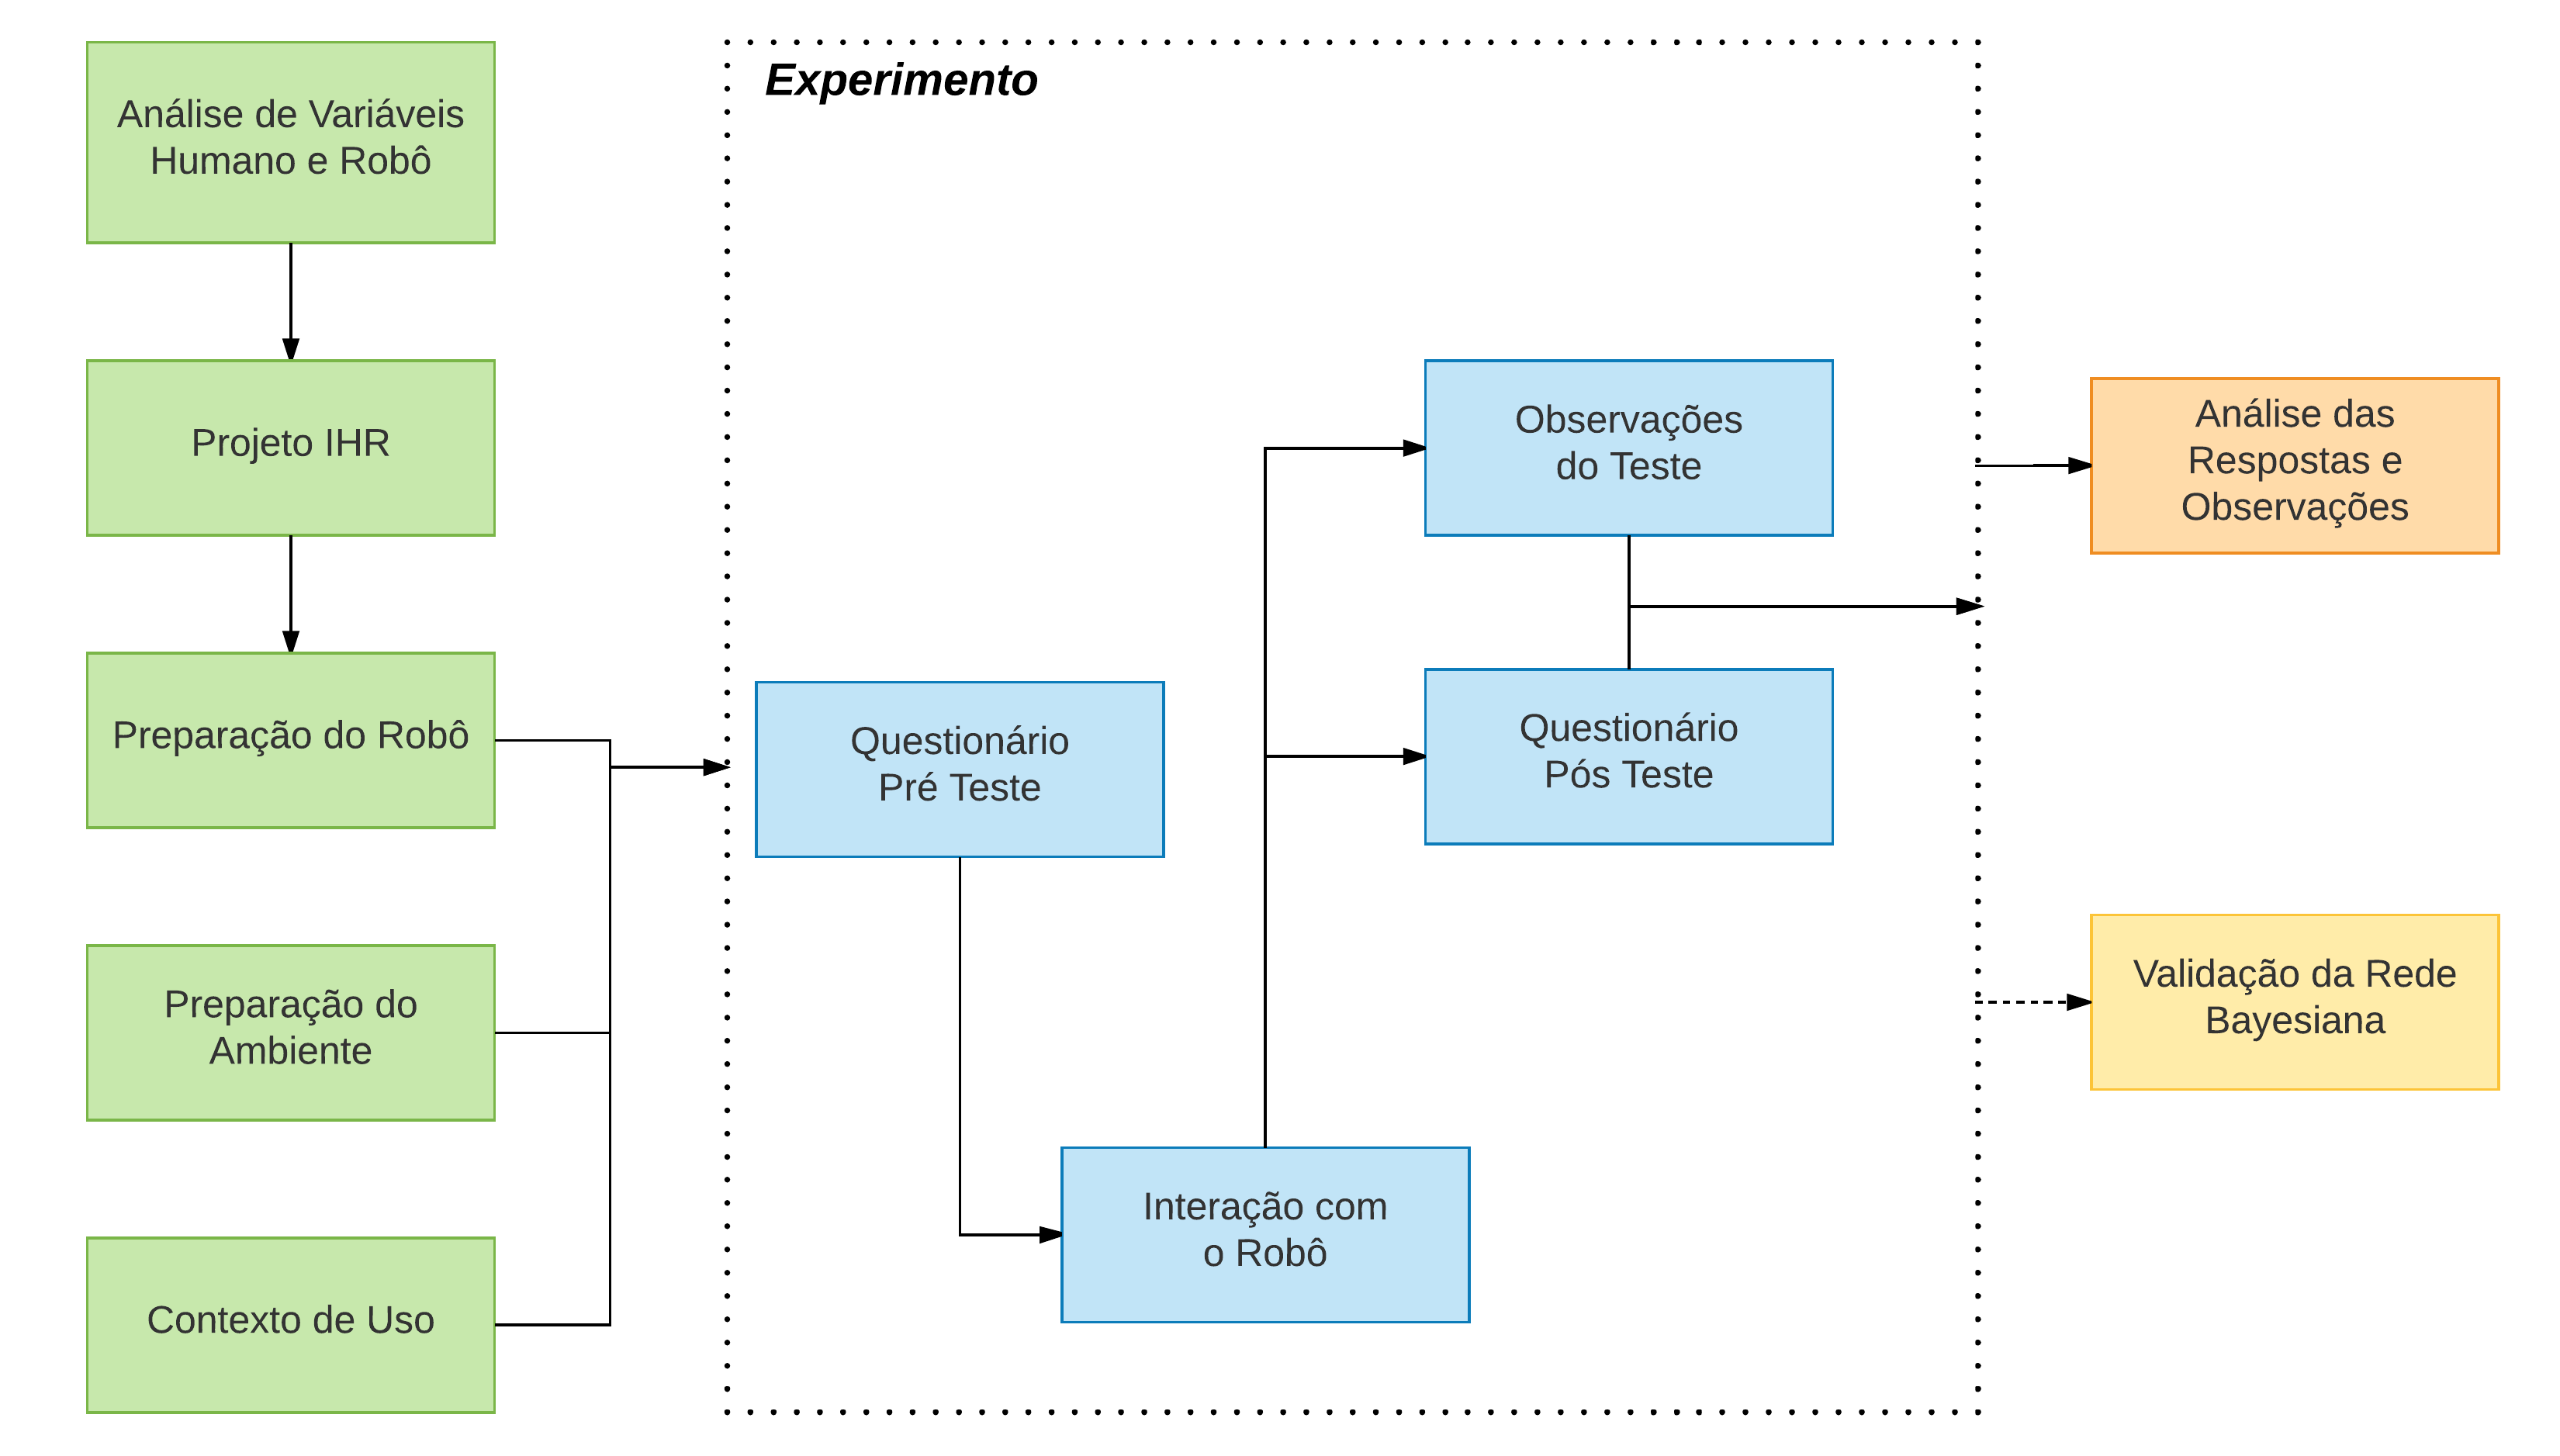
\includegraphics[width=\textwidth]{experimento.png}
		\smallcaption{Fonte: o autor.}
		\label{fig:experimento}
	\end{minipage}
\end{figure}

A figura~\ref{fig:experimento} apresenta a sequência de passos executadas para a concepção do experimento dessa tese. Os primeiros passos auxiliam a definir o escopo do teste e o que será avaliado ao longo do experimento. Esses primeiros passos estão definidos através da cor verde. Em cor azul, estão os passos realizados para execução do teste de interação entre o robô e o ser humano. Por fim, temos duas etapas em tons amarelo e laranja. O amarelo corresponde aos testes de validação do classificador bayesiano e serão discutidos no capítulo~\ref{cap:proposta}. A etapa laranja é referente a análise do especialista após a coleta de informações no teste de IHR. A seguir, cada uma das etapas será discutida e apresentada ao longo do capítulo separadas em seções.

\section{Análise de Variáveis para IHR}
\label{sec:variáveis}
O primeiro passo para construir o experimento é identificar o conjunto de variáveis que possam auxiliar a identificar informações sobre a IHR. Essas variáveis devem ser separadas em classes de maneira que seja possível referência-las em outros momentos do projeto. Além da referência, as classes são importantes pois, ajudam a definir o tipo de projeto que será investigado durante o experimento. A investigação tem o objetivo de melhorar a IHR sempre com o foco nas necessidades do ser humano, o usuário do sistema. Cada classe de variáveis adotada possuí um método diferente para obtenção das informações. Contudo, esse método de captura não é restrito e podem ser discutidos diferentes meios de obtenção da informação. Por exemplo, a variável nome do usuário, pode ser obtida através da interação por voz com o usuário ou através de questionário. O meio de obtenção dependerá do momento e objetivo do experimento.

Para selecionar as variáveis, é realizado um trabalho de revisão bibliográfica e identifica-se como representar as informações necessárias ao problema. Na aproximação do robô, algumas variáveis foram identificadas ao longo do capítulo~\ref{cap:proxemics}. O uso da teoria de proximidade torna possível a extração de fatores comportamentais com base na distância social entre a pessoa e o robô. Esses fatores podem variar não só entre a posição física dos dois agentes, mas também na posição do corpo dos indivíduos, como por exemplo, a orientação dos ombros e troco em relação a posição do robô (linguagem corporal)~\cite{mead:2016}. Outro fator significante é a fixação entre olhares, este pode auxiliar no processo que determina o início e o fim de uma interação. O olhar também auxilia a determinar quem são os principais indivíduos na interação~\cite{mumm:2011, srinivasan:2012}. Pode-se empregar o reconhecimento de expressões faciais para auxílio na análise do quanto a situação é confortável para o indivíduo, ou o quanto o usuário aprecia a interação. Existir uma avaliação em tempo real das reações deste indivíduo durante todo o processo de interação, auxilia na compreensão da experiência do usuário~\cite{amaral:2014}. Outra técnica para análise de conforto na interação é a avaliação da emoção através da voz da pessoa, ou através do uso de equipamento de eletroencefalografia~(EEG), porém este último é um método mais invasivo já que exige a adição de um equipamento na pessoa que interage com o robô~\cite{bos:2006, lee:2014}.

É possível empregar diversos sensores que auxiliam a leitura e quantificação dessas variáveis. Sensores de captura de marcações de movimento, como Microsoft\textregistered\ Kinect\textregistered\ ou o ASUS\textregistered\ Xtion\textregistered, são utilizados para quantificar os valores comportamentais obtidos através das variáveis, que envolvem distância entre agentes e orientação de membros do indivíduo. Para realizar o reconhecimento de expressões faciais utiliza-se uma câmera de video, podendo assim executar uma leitura da face da pessoa em tempo de execução. As variáveis referentes a questão da fixação dos olhares dos agentes para identificar o início e o fim da interação, podem ser obtidas através de ambos sensores, sendo possível determinar a orientação da cabeça e torso do indivíduo, além de também a direção do olhar da pessoa para o robô. A voz do indivíduo para análise da emoção na interação é obtida através de um microfone direcional ou um arranjo de microfones, que amplifica a capacidade de percepção do robô em relação ao ambiente e a pessoa que interage com ele.

As variáveis aplicadas ao comportamento tem dependência do cenário de interação, porém as informações das variáveis etnográficas como idade, experiência computacional, sexo, local de origem, etnia, entre outras, são independentes do cenário. Existem alguns algoritmos na área de visão computacional que são capazes de identificar algumas variáveis etnográficas de maneira automática \cite{yang:2007, shan:2012, ylioinas:2012, samadi:2013, amaral:2014}, isso pode auxiliar no processo de expansão da rede bayesiana de maneira automática. Porém, nem todas as informações podem ser obtidas de maneira automática, então alguns métodos como questionários e entrevistas são necessários para melhor compreendimento do comportamento do usuário e identificar como foi sua experiência durante a interação.

Cada uma das variáves será discutida conforme apresentadas nas seções a seguir.

\subsection{Variáveis Etnograficas}
\label{sec:etnograficas}
As variáveis etnográficas tem o objetivo de coletar informações sobre etnia, cultura, costume e outros fatores antropológicos~\cite{borges:2005}. Além dessas informações, esse tipo de variável auxilia na identificação de dados sobre idade, gênero, experiência social e também tecnológica do indivíduo. Todas as informações representadas nos dados etnográficos são relevantes para verificar a adesão do usuário sobre tecnologias novas, qual cultura ele está inserido, e outras informações que podem determinar o nível de interação que ele aceita. Essas informações podem ser capturadas através de questionários e entrevistas. Caso seja uma necessidade do projeto, o robô pode realizar a entrevista para coletar essas informações. Para o desenvolvimento dessa tese, como essas informações são para analises do especialista, optou-se pela coleta através do questionário. A lista apresentada a seguir define as variáveis etnográficas e uma breve explicação sobre o significado de cada uma.

\begin{enumerate}
	\item \textbf{Idade}: informa a idade do indivíduo.
	\item \textbf{Gênero}: informa o sexo biológico do indivíduo.
	\item \textbf{Local de Nascimento}: informa qual o local de nascimento do indivíduo. Essa variável auxiliará a determinar a base cultural do indivíduo.
	\item \textbf{Etnia}: informa a origem da família do indivíduo. Outra variável que auxilia na determinação da base cultural do indivíduo.
	\item \textbf{Quantidade de \emph{Gadgets}}: informa a quantidade de \emph{gadgets} que o indivíduo possui, ajudando a identificar qual a experiência e o contato dele com a tecnologia.
	\item \textbf{Contato prévio com Robôs}: informa apenas se o indivíduo já possuiu algum contato com robôs. Auxiliará a determinar o contato com a tecnologia, principalmente com robôs que poderá influenciar no seu comportamento durante a interação.
	\item \textbf{Tipos de Robôs}: informa quais são os tipos de robôs que o indivíduo teve contato. Os tipos poderão ser robôs \emph{Pet}, Humanoides, Androides, Móveis, entre outros. Essa variável é um complemento da variável ``Contato prévio com Robôs''.
	\item \textbf{Quantidade de cidades visitadas}: informa a quantidade de cidades que o indivíduo já visitou além da sua cidade natal. É importante para identificar o contato com outros tipos de cultura. Isso poderá influenciar no comportamento definido por sua cultura.
	\item \textbf{Quantidade de cidades que morou}: informa a quantidade de cidades que o indivíduo já morou além da sua cidade natal. É importante para identificar a vivência com outros tipos de cultura. Isso poderá influenciar no comportamento definido por sua cultura.
	\item \textbf{Quantidade de países visitadas}: informa a quantidade de países que o indivíduo já visitou além da sua cidade natal. É importante para identificar o contato com outros tipos de cultura. Isso poderá influenciar no comportamento definido por sua cultura.
	\item \textbf{Quantidade de países que morou}: informa a quantidade de países que o indivíduo já morou além da sua cidade natal. É importante para identificar a vivência com outros tipos de cultura. Isso poderá influenciar no comportamento definido por sua cultura.
\end{enumerate}

Em diversos trabalhos da seção \ref{sec:proxemicsihr}, onde a questão cultural do indivíduo é abordada, são discutidos que influência a cultura provê sobre o comportamenteo do o indivíduo. A cultura é tratada como a origem do indivíduo~\cite{eresha:2013}. Entretanto, a questão cultural na vida de uma pessoa é mais abrangente pois, pode ser relacionada com a experiência adquirida ao longo de sua vivência social, como por exemplo, países e cidades que o indivíduo visitou e viveu, o meio ao qual ele está inserido, sua profissão, entre outras informações. Dessa forma, o conjunto de variáveis apresentado na lista acima auxilia a mapear de forma abstrata a experiência social do indivíduo. O intuito do uso das informações etnográficas é investigar até que ponto elas podem influenciar na experiência do usuário durante a interação com o robô.

\subsection{Variáveis Comportamentais}
\label{sec:reacoes}
Variáveis comportamentais tem como principal objetivo identificar reações de comportamento dentro do cenário exigido por uma determinada tarefa. As variáveis comportamentais são coletadas a partir de informações sobre expressões corporais, expressões faciais e também de declaração explicita da pessoa ou do robô. O uso dessa classe de variáveis possibilita uma análise baseando-se em teorias de linguagem corporal e de microexpressões. Algumas possibilidades para analisar expressões corporais são discutidas no trabalho apresentado por \citeonline{lambert:2008}. O conjunto de variáveis comportamentais apresentados nessa seção podem ser utilizados não apenas para extrair o perfil do indivíduo, mas também para avaliar a ação realizada pelo robô ao interagir com o usuário. Dependendo do \emph{hardware} utilizado no robô, essas variáveis também possibilitam que o robô realize esses comportamentos durante a interação. A lista apresentada a seguir define as variáveis comportamentais obtidas através da literatura e uma breve explicação sobre o objetivo de cada uma das variáveis.

\begin{enumerate}
	\item \textbf{Expressões Faciais}: é possível identificar se a reação do indivíduo foi positiva ou negativa, a partir de uma ação do robô. Existem seis expressões bases que combinadas formam diversas outras~\cite{bihan:2014}. Contudo, nesse trabalho será considerado apenas as seis expressões bases classificadas em dois grupos: expressões faciais positivas e expressões faciais negativas. O intuito dessa variável é realizar a avaliação da ação do robô com base nas expressões faciais do indivíduo.
	\item \textbf{Tempo de Transição entre as Zonas Sociais}: identificar o tempo que o indivíduo ficou confortável com a presença do robô a medida que esse diminuiu a distância entre eles.
	\item \textbf{Frequência do Olhar em direção ao Robô}: identificar se o indivíduo mantém o olhar ao robô, sendo possível saber se a interação está continua ou não. Isso pode influenciar se o robô está interagindo de maneira confortável ao indivíduo ou se esse está incomodado com a presença do robô.
	\item \textbf{Tempo do Olhar}: é possível mensurar o interesse do indivíduo durante a interação através do tempo que ele permanece com o olhar fixo no robô. Quanto maior o tempo do olhar, maior o interesse na interação do indivíduo.
	\item \textbf{Orientação dos ombros}: Auxilia a mensurar o interesse do indivíduo durante a interação, analisando se os ombros possuem a mesma orientação que a cabeça e também uma orientação em direção ao indivíduo que interage com o robô. Além disso, é possível determinar através do alinhamento do quadril com o ombro do indivíduo o ângulo de inclinação de seu torso. A inclinação do torso auxilia a identificar o interesse do indivíduo na interação, para isso basta verificar se ele está inclinado em direção ao robô para determinar um interesse positivo.
	\item \textbf{Orientação do quadril}: Auxilia a mensurar o interesse do indivíduo durante a interação. A orientação do quadril em direção ao robô ou na direção oposta auxilia a determinar o grau de interesse do indivíduo na interação. Quando mais alinhado à direção do robô, maior o interesse do indivíduo na interação.
	\item \textbf{Estilo da Voz}: é importante, pois pode determinar a reação que o indivíduo terá após a interação via áudio com o robô. Além disso, é possível determinar se o indivíduo está confortável ou não durante a interação, analisando o tom de sua voz ao responder o robô. Nesse trabalho, será considerado somente o canal de resposta ao indivíduo.
    \item \textbf{Conforto}: determina se o indivíduo está disposto a continuar a interação ou se algo o incomoda, fazendo com que desista de interagir com o outro agente. Essa é uma informação que pode ser obtida através das demais apresentadas acima ou declarada diretamente pelo usuário, como no caso do projeto desta tese.
    \item \textbf{Medo}: determina se o indivíduo sente-se seguro durante a interação com o outro agente. Pode impactar diretamente a experiência de interação do usuário. Essa é uma informação que pode ser obtida através das demais apresentadas acima ou declarada diretamente pelo usuário, como no caso do projeto desta tese.
\end{enumerate}

As variáveis apresentadas acima podem auxiliar na descoberta do interesse em relação a interação. Algumas delas, como as que envolve o olhar, podem necessitar de equipamentos mais específicos para obter uma melhor acurácia na captura. Outras variáveis necessitam de técnicas e estudos direcionados para trazer a interação à um nível mais natural, como o caso da voz. Dessa forma, escolher quais variáveis trabalhar tem influência não só sobre o estudo realizado, como também nos equipamentos embarcados no robô. Tais equipamentos, podem influenciar em sua aparência e consequentemente na experiência do usuário.

\subsection{Variáveis do Robô}
\label{sec:variaveisrobo}
Além das variáveis referentes etnográficas e comportamentais, deve-se considerar também as informações sobre o robô uma vez que sua aparência pode influenciar na reação e expectativa das pessoas durante a interação~\cite{hegel:2009}. Variáveis do robô podem auxiliar a identificar quais são os principais fatores que tornam a interação humano-robô uma boa experiência ao usuário e também natural. Um conjunto de variáveis é apresentado com o objetivo de caracterizar fatores do robô, referente a sua aparência, que influenciam na interação social. Esse conjunto de variáveis é apresentado a seguir:

\begin{enumerate}
	\item \textbf{Altura}: A altura do robô para identificar a influência da diferença entre alturas de robôs e humanos.
	\item \textbf{Volume}: O volume ocupado pelo robô pode influenciar no conforto da interação, uma vez que quando o robô atingir uma zona social mais próxima do indivíduo pode causar uma sensação claustrofóbica a ele.
	\item \textbf{Tipo do Robô}: Segundo \citeonline{choi:2014}, robôs possuem dois tipos: Autônomos e Tele-operados. Essa variável define o quanto de intervenção humana é necessário para que o robô possa executar a tarefa objetivo.
	\item \textbf{Classificação do Robô}: Segundo \citeonline{dobra:2014} classificar um robô é uma tarefa muito complexa e pode envolver diversas variáveis. Dessa forma, para essa tese será considerado uma classificação mais simples. O robô deve ser classificado como: fixo, móvel com rodas, móvel bípede, móvel quadrupede, móvel com manipuladores. Outras classificações podem ser inseridas conforme a necessidade e inclusão de novos robôs.
	\item \textbf{Aparência Física}: Essa variável descreve se o robô possui uma aparência amigável ou agressiva.
	\item \textbf{Nível de Ruído}: Determina qual o nível de ruído que os atuadores do robô podem gerar de tal forma, que possa influenciar na interação humano-robô. Como exemplo, pode-se citar o Big Dog~\footnote{http://www.bostondynamics.com/robot\_bigdog.html}, da Darpa Robotics, que é movido através de um motor diesel e seus atuadores pneumáticos e hidráulicos apresentam um alto grau de ruído.
\end{enumerate}

\subsection{Variáveis de Ações na Interação}
\label{sec:acoes}
Existem variáveis que determinam as possíveis ações que o robô e o ser humano podem executar. Essas ações podem gerar comportamentos diferentes de acordo com o contexto ao qual o cenário está inserido. No caso do robô, as possíveis ações são determinadas a partir do \emph{hardware} disponível para o projeto. Fatores como tipo de manipulador, sonorização, saída de vídeo, entre outros, determinam quais são as ações que o robô deve ter. As variáveis que compõem as informações do perfil comportamental do robô são:

\begin{enumerate}
	\item \textbf{Aproximação}: Forma de aproximação do robô ao indivíduo. Pode ser classificada entre rápida, devagar, brusca ou suave.
	\item \textbf{Movimentação do Manipulador}: Caso exista um manipulador deve descrever como é feita a movimentação do manipulador em direção ao usuário. A classificação pode ser feita entre brusca e suave; ou em relação a sua amplitude, como longo e curto.
	\item \textbf{Estilo de Voz}: Ao emitir algum tipo de som o robô deverá manter um estilo de voz para que seja possível simbolizar qual o tipo de mensagem ele deseja falar. A classificação será feita de maneira simplificada, considerando apenas se é um estilo educado ou agressivo.
	\item \textbf{Volume de Voz}: Ao emitir um som, o robô deve saber qual o volume adequada considerando a interação, ambiente e distância do segundo agente. Uma classificação simples pode ser utilizada, como por exemplo, alto e baixo.
	\item \textbf{Expressão Facial}: Ao iniciar o contato visual com o indivíduo, pode ocorrer diversas expressões do robô na tentativa de manter o conforto do indivíduo durante o processo de interação. Simplificando as expressões são consideradas apenas dois tipos de expressões realizadas pelo robô: amistoso e não-amistoso. As expressões faciais do robô serão executadas através do \emph{tablet} acoplado nele, conforme descrito na seção~\ref{sec:robo}.
\end{enumerate}

A partir das variáveis identificadas, deve-se realizar a definição do contexto de uso, do ambiente e também do robô que serão utilizados no projeto para definir quais e como são utilizadas cada uma das variáveis no projeto de IHR proposto por essa tese.

\section{Contexto de Uso}
\label{sec:contextouso}
Para que a interação com o sistema seja de melhor qualidade, um ponto importante do projeto é definir o contexto de uso. Ele determina quando e onde será realizado a interação com o sistema, no caso desta tese, o robô. O contexto de uso é importante, pois pode influenciar no tipo de comportamento e expectativa do usuário para com o sistema~\cite{barbosa:2010}.

A definição do contexto de uso é baseada em um texto descritivo que delimita todo o cenário da aplicação e como foi planejado o experimento. Esse cenário descreve quem é o usuário, quais os pontos de interação com o sistema e também como será o comportamento do usuário e também do robô. O contexto descrito delimita todo o escopo do teste. Ele assegura que as observações tenham o objetivo de garantir a qualidade do uso dentro daquele cenário. A figura~\ref{fig:contextouso} apresenta o cenário aplicado no contexto de uso dessa tese.

\begin{figure}[ht!]
	\centering
	\begin{minipage}{\textwidth}
		\caption{Ilustração do contexto de uso}
		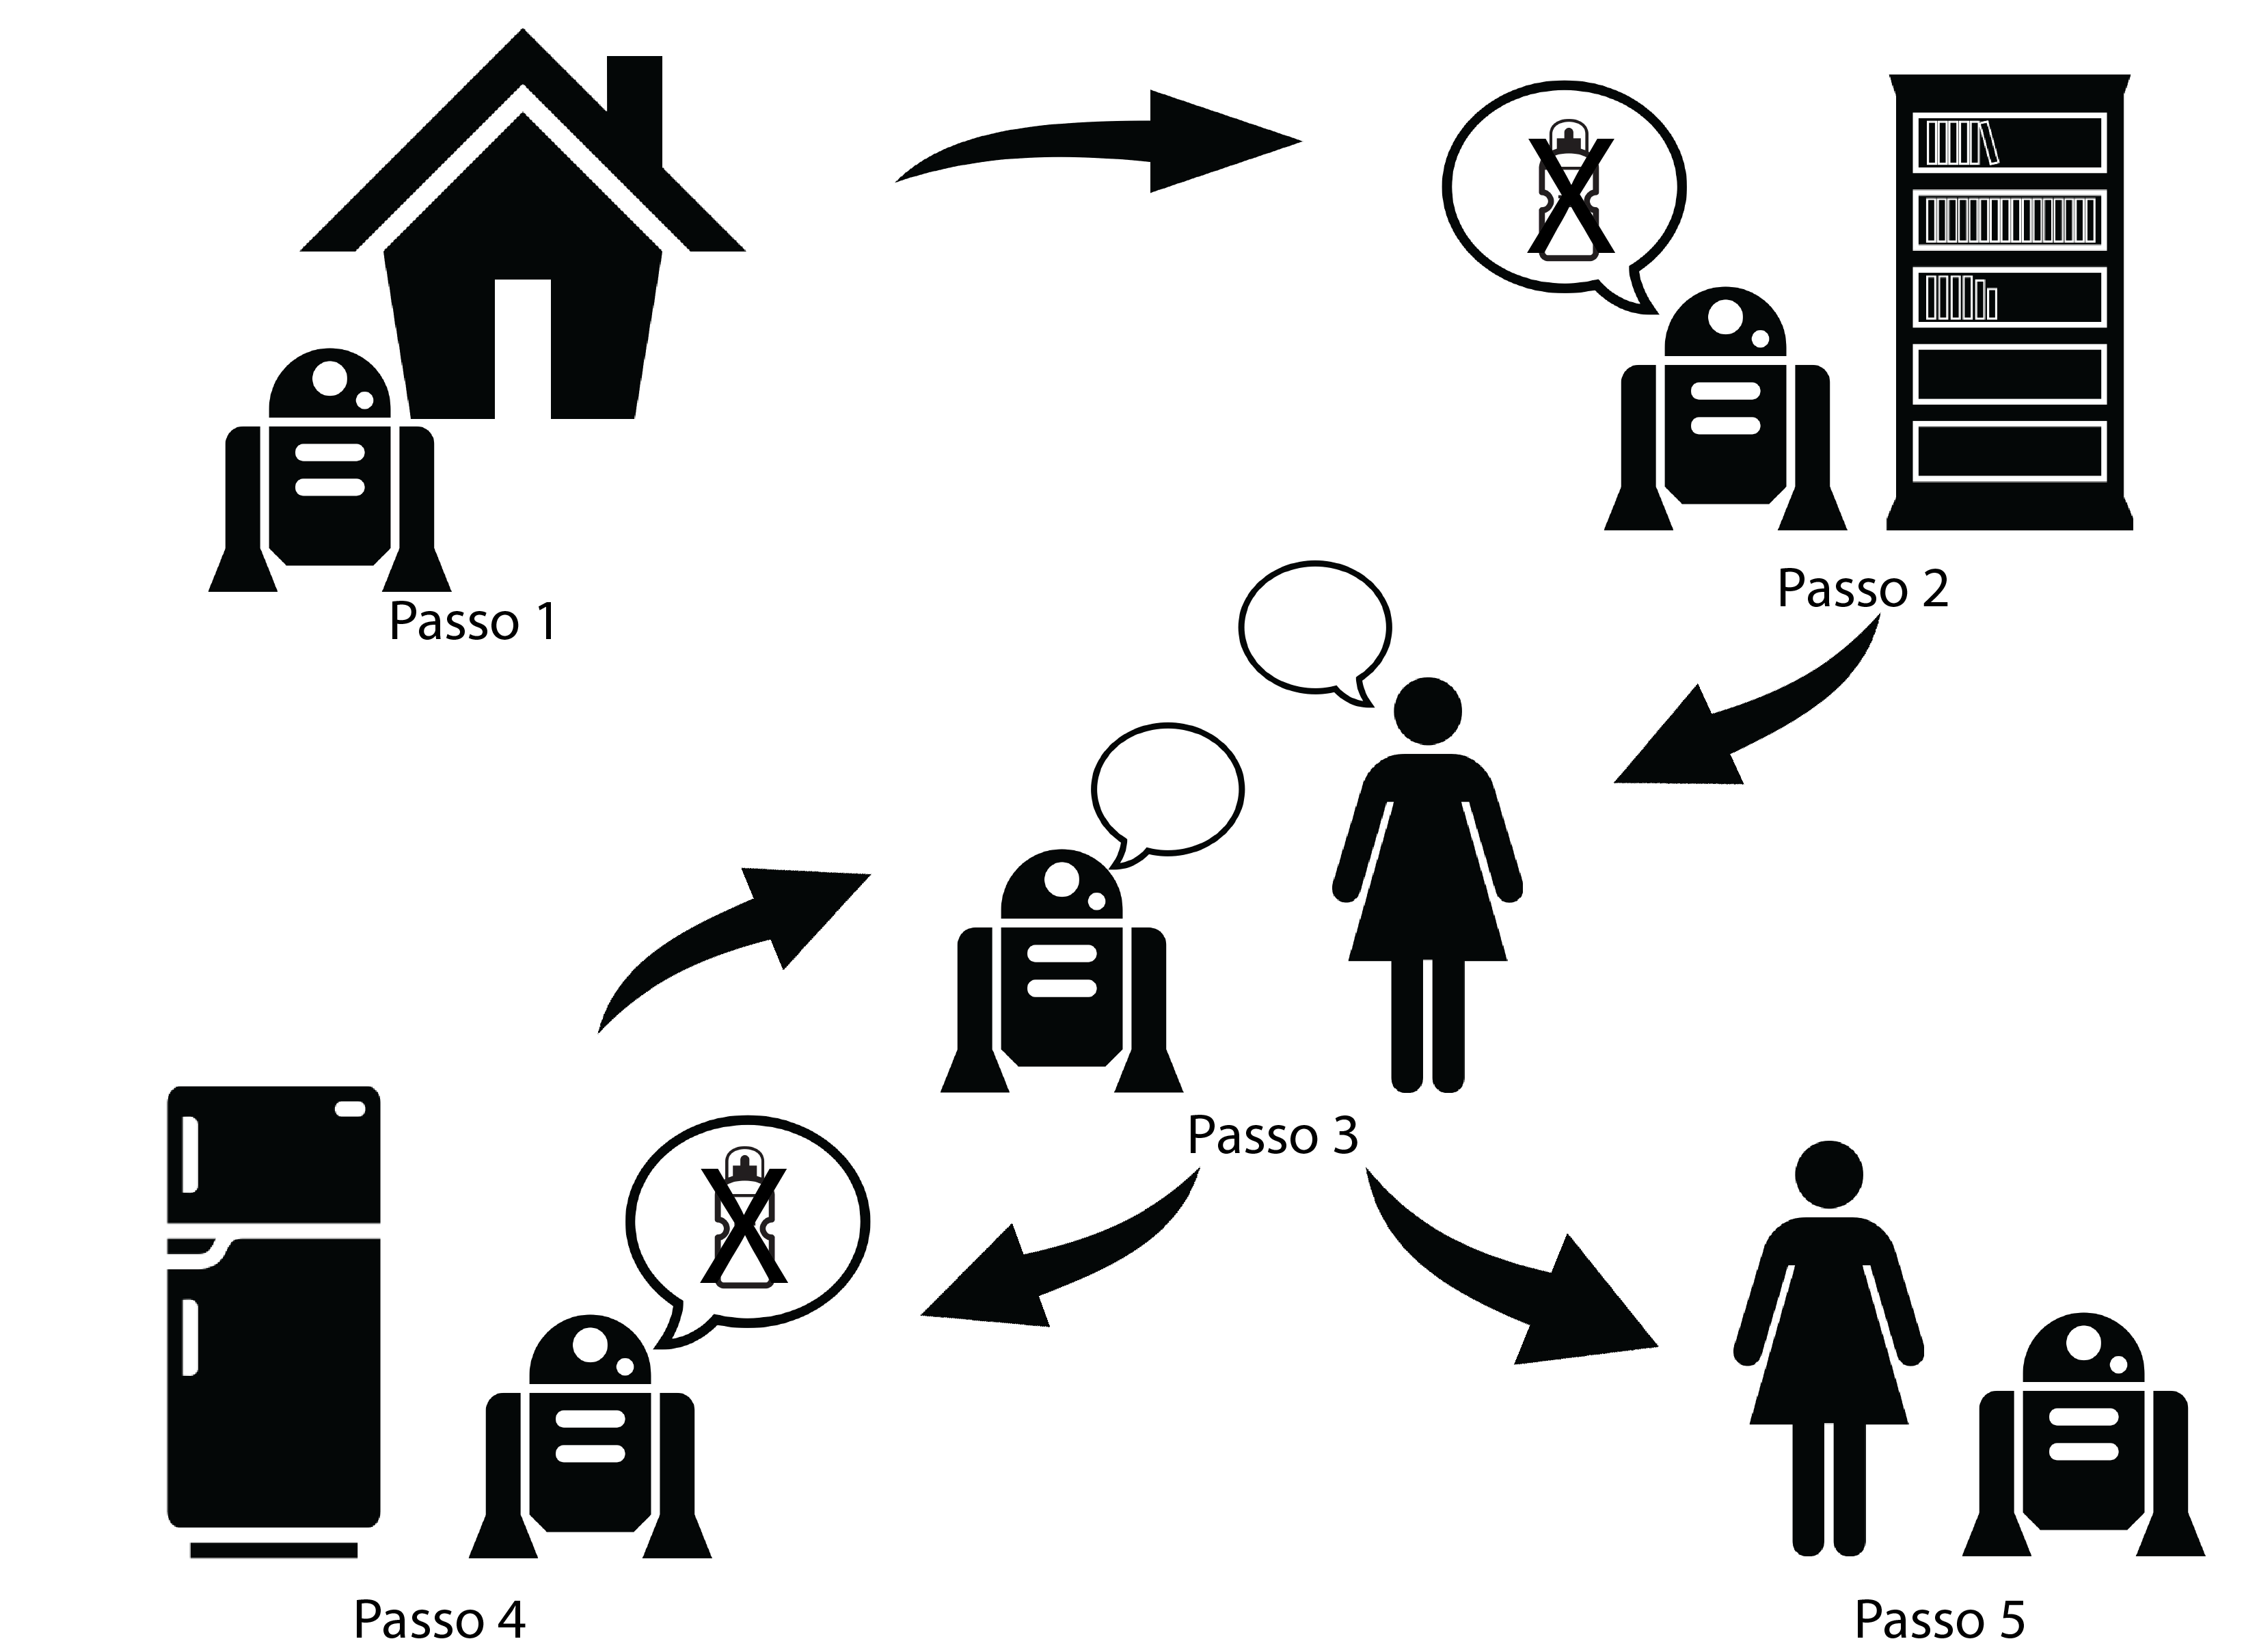
\includegraphics[width=\textwidth]{contexto-uso.png}
		\smallcaption{Fonte: o autor.}
		\label{fig:contextouso}
	\end{minipage}
\end{figure}

O cenário apresentado na figura~\ref{fig:contextouso} ilustra uma situação onde o robô entra em sua casa (passo 1) e vai até a estante onde ele deixou uma garrafa. A garrafa não está mais no local que ele deixou (passo 2), então ele vai até a pessoa que convive com ele no ambiente da casa. Ao interagir com a pessoa, o robô pergunta se ela viu a garrafa e recebe uma resposta negativa (passo 3). Na sequência, o robô procura pela garrafa em outro cômodo da casa, onde também não encontra (passo 4). O robô então retorna ao encontro da pessoa, e solicita a ajuda para procurar pela garrafa (passo 3). Como última etapa, a pessoa atende o pedido e ambos saem para procurar pela garrafa (passo 5), finalizando assim o cenário.

Através dessa ilustração pode-se definir o contexto de uso desta tese, onde o robô realiza a aproximação de pessoas que convivem com ele dentro de uma casa. Essa aproximação é realizada com o objetivo de solicitar ajuda ao humano para encontrar um objeto que foi deixado em algum lugar da casa. Com as variáveis identificadas e o contexto de uso da tese definidos, é necessário realizar a especificação do projeto, considerando fatores de engenharia de \emph{software} e fatores humanos já que existe interação humano-robô.

\section{Especificando o Projeto de IHR}
\label{sec:projetoihr}
Nos capítulos sobre IHR (capítulo~\ref{cap:ihr}) e teoria de proximidade (capítulo~\ref{cap:proxemics}) são apresentados diversos trabalhos com o estudos sobre interação entre humanos e robôs em diversas áreas, como saúde, lazer, entreterimento e social. Porém, ao analisar os projetos feitos nos trabalhos relacionados, não existe nenhuma definição sobre a especificação do projeto, como requisitos, perfis de usuários atentidos com o projeto, entre outros. O contexto de uso, em alguns casos, é utilizado pois, o projeto tem um foco em uma determinada tarefa. Contudo, projetos sem especificações são difícies de serem reproduzidos, um vez que os robôs utilizados são bem específicos. Além de serem específicos, os robôs utilizados são construídos, nos laboratórios das universidades e centros de pesquisas, em parte das pesquisas. As demais pesquisas utilizam robôs como: Softbank NAO~\footnote{https://www.ald.softbankrobotics.com/en/robots/nao} e PR2~\footnote{http://www.willowgarage.com/pages/pr2/overview}, que são produzidos por empresas especializadas fazendo com que o projeto fique restrito a sua capacidade determinada pela fábrica.

Em engenharia de \emph{software} são estudados vários métodos que auxiliam na especificação do projeto. Nesses métodos são encontrados a contemplação de alguns princípios que garantem a reprodução, manutenção e evolução do projeto ao longo tempo. Os princípios de engenharia de \emph{software} não são vistos como regras, mas como boas práticas para o desenvolvimento do projeto~\cite{wazlawick:2013}. As boas práticas aplicadas em sistemas computacionais, também podem ser aplicadas no desenvolvimento de projetos de robôs.

%!TEX root=Principal.tex
\chapter{PROPOSTA}
\label{cap:proposta}

Este trabalho apresenta uma metodologia que mapeia o conjunto de ações que o robô é capaz de executar visando a maximização a qualidade da interação humano-robô, baseando-se no comportamento e características do indivíduo. Como observado ao longo dos trabalhos da literatura apresentados até agora, o comportamento do indivíduo possui dependência da origem ou cultura dele. Assim, algumas reações apresentadas por uma pessoa podem ser influenciadas pelo local de nascimento, pelos locais que o indivíduo viveu e também pela sua experiência de vida. Contudo, fatores como a experiência de vida e cultura são difíceis de avaliar apenas com a observação de uma determina pessoa.

Dessa forma, a técnica de Raciocínio baseado em Casos (RBC) foi escolhida como apoio a essa tese, para que seja possível armazenar as experiências de interações entre robô e as pessoas, e a partir da informação gerada com base nos casos, identificar a melhor forma de interagir com novas pessoas de acordo com seu perfil comportamental. Entretanto, o número de informação gerada no processo de interação com diversas pessoas é consideravelmente alto, isso dificulta a consulta dos casos para reutilizar a solução em tempo de interação entre o ser humano e o robô. Com o intuito de minimizar a quantidade de casos para encontrar a provável melhor interação tendo como base um determinado perfil e otimizar o tempo de procura dessa solução é utilizado um algoritmo de agrupamento que será capaz de gerar grupos de perfis comportamentais. É a partir desses perfis que o mecanismo de classificação identifica o melhor conjunto de ações para o robô executar referente àquele caso. 

Essa seção apresenta em detalhes os passos da metodologia proposta por esta tese. Ao final do capítulo é apresentado a visão completa da metodologia onde é realizado uma síntese do processo como um todo e das técnicas aplicadas nele. Antes de entrar em detalhes na metodologia, é apresentado o robô que será utilizado para o desenvolvimento do estudo proposto nessa tese.

\section{O Robô}
\label{sec:robo}
O robô utilizado no desenvolvimento dessa tese é o PeopleBot~\footnote{PeopleBot - http://www.mobilerobots.com/researchRobots/PeopleBot.aspx} fabricado pela ActivMedia Robotics. Ele é um robô móvel com direção diferencial, ou seja, possui duas rodas motorizadas e uma roda castor que auxilia no equilíbrio do robô. O projeto do PeopleBot tem foco em pesquisas e serviços que envolvem interação humano-robô, devido a isso ele possui uma altura de 112 cm (centímetros). Além disso, o PeopleBot também possui uma garra pequena que tem sua movimentação apenas na vertical. A figura~\ref{fig:peoplebot} apresenta o robô PeopleBot.

\begin{figure}[ht!]
	\centering
	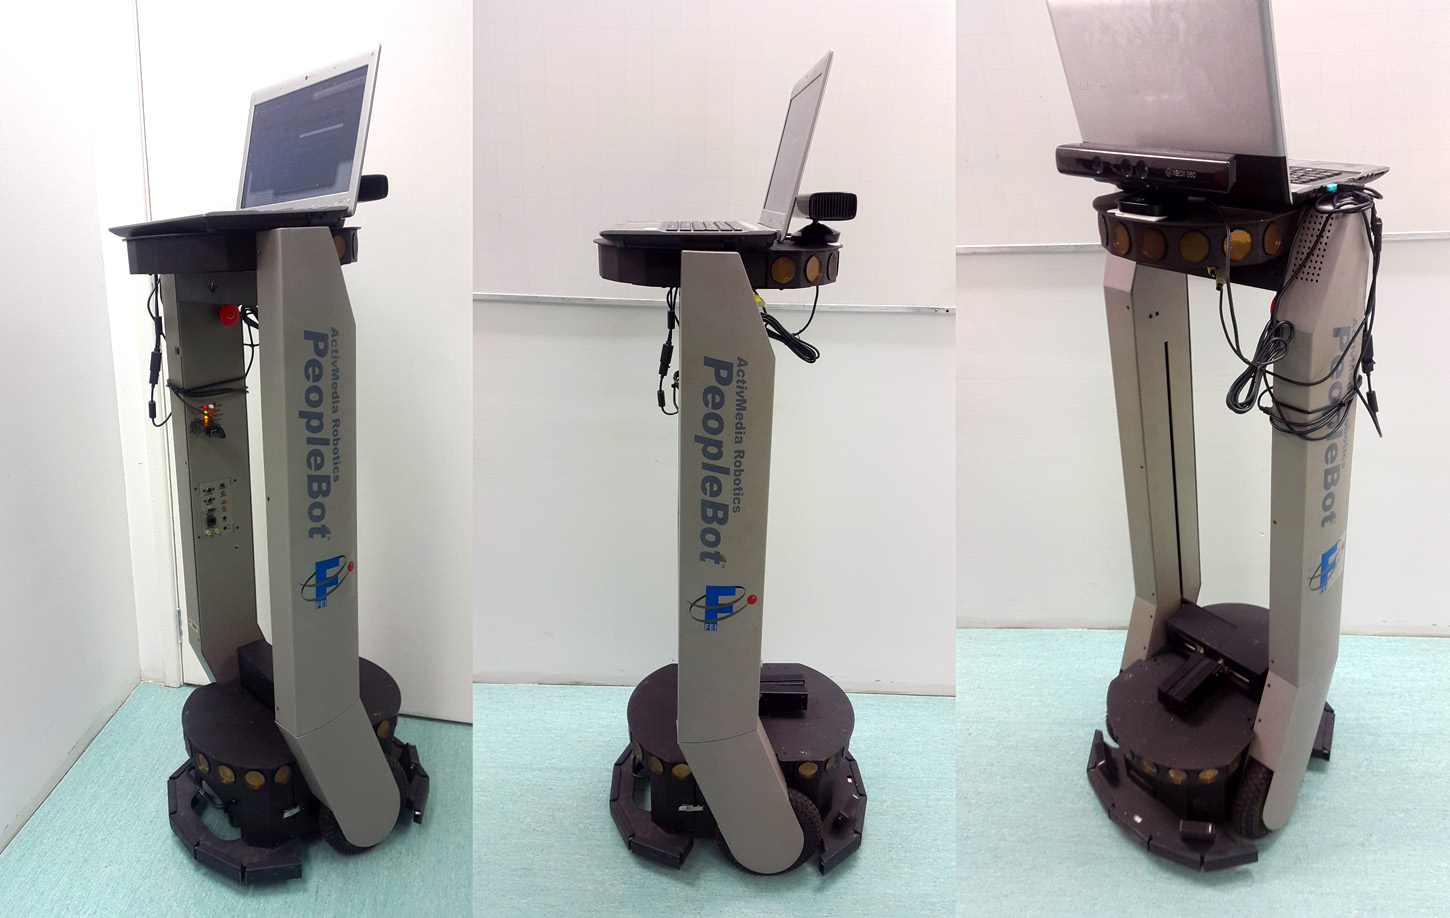
\includegraphics[width=\textwidth]{images/peoplebot.jpg}
	\caption{Robô ActivMedia Robotics PeopleBot.}
	\label{fig:peoplebot}
\end{figure}

Como a garra do PeopleBot é curta e não permite muitos movimentos, foi adicionado um manipulador para auxiliar na manipulação de objetos durante a interação com as pessoas e também na prestação de serviços domésticos e de cuidados pessoais. O projeto de construção do manipulador é apresentado através da figura~\ref{fig:manipulador}.

\begin{figure}[ht!]
	\centering
	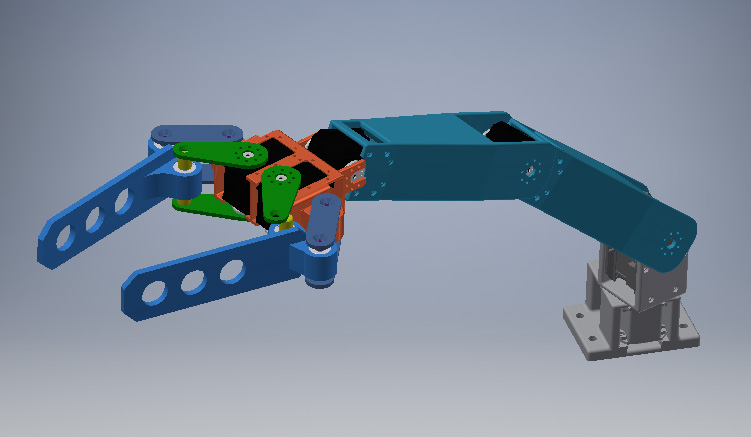
\includegraphics[width=0.6\textwidth]{images/manipulador.jpg}
	\caption{Projeto do Novo Manipulador do PeopleBot.}
	\label{fig:manipulador}
\end{figure}

O novo manipulador foi construído de maneira que os movimentos sejam parecidos com o braço humano. Além do manipulador, também será acoplado um \emph{tablet} para que seja possível atribuir faces ao robôs e deixar a interação mais amigável. Alguns sensores como o Microsoft\textregistered\ Kinect\textregistered\ e o ASUS\textregistered\ Xtion\textregistered\ também foram instalados para melhorar a captura das informações que são apresentadas na seção~\ref{sec:extracaocaracteristicas}, a seguir.

\section{Extração das Características para o RBC}
\label{sec:extracaocaracteristicas}

Como apresentado na seção \ref{cap:ihr}, existem diversas variáveis que podem auxiliar na extração de um perfil comportamental do individuo. \emph{Proxemics} tornam possível a extração de fatores sobre a distância social entre o individuo e o robô. Esses fatores podem variar não só entre a posição física dos dois agentes, mas também na posição do corpo dos indivíduos, como por exemplo, a orientação dos ombros e troco em relação a posição do robô. Outro fator também significante é a fixação entre olhares, este pode determinar o início e o fim de uma interação, além dos principais indivíduos na interação. Além disso, pode ser também empregado o reconhecimento de expressões faciais que auxiliam na análise do quanto a situação é confortável para o individuo, ou seja, o quanto ele está apreciando a interação, de tal forma, que possa existir uma avaliação em tempo real das reações deste durante todo o processo de interação. Outra técnica que pode ser utilizada na análise do conforto do individuo durante a interação é a avaliação da emoção através da voz da pessoa.

Dessa forma, é possível empregar diversos sensores que auxiliam a leitura e quantificação dessas variáveis. Sensores de captura de marcações de movimento, como Microsoft\textregistered\ Kinect\textregistered\ ou o ASUS\textregistered\ Xtion\textregistered, são utilizados para quantificar os valores obtidos através da \emph{Proxemic}, que envolvem distância entre agentes e orientação de membros do individuo. Para realizar o reconhecimento de expressões faciais utiliza-se uma câmera de video, podendo assim executar uma leitura da face do individuo em tempo de execução na interação entre o humano e o robô. As variáveis referentes a questão da fixação dos olhares dos agentes para identificar o início e o fim da interação, podem ser obtidas através de ambos sensores de tal forma, que seja possível determinar a orientação da cabeça e torso do individuo e também a direção do olhar deste para com o robô. A voz do individuo para análise da emoção na interação é obtida através de um microfone. A figura \ref{fig:capturacaracteristicas} apresenta a ilustração do processo de extração das características do individuo.

\begin{figure}[ht!]
	\centering
	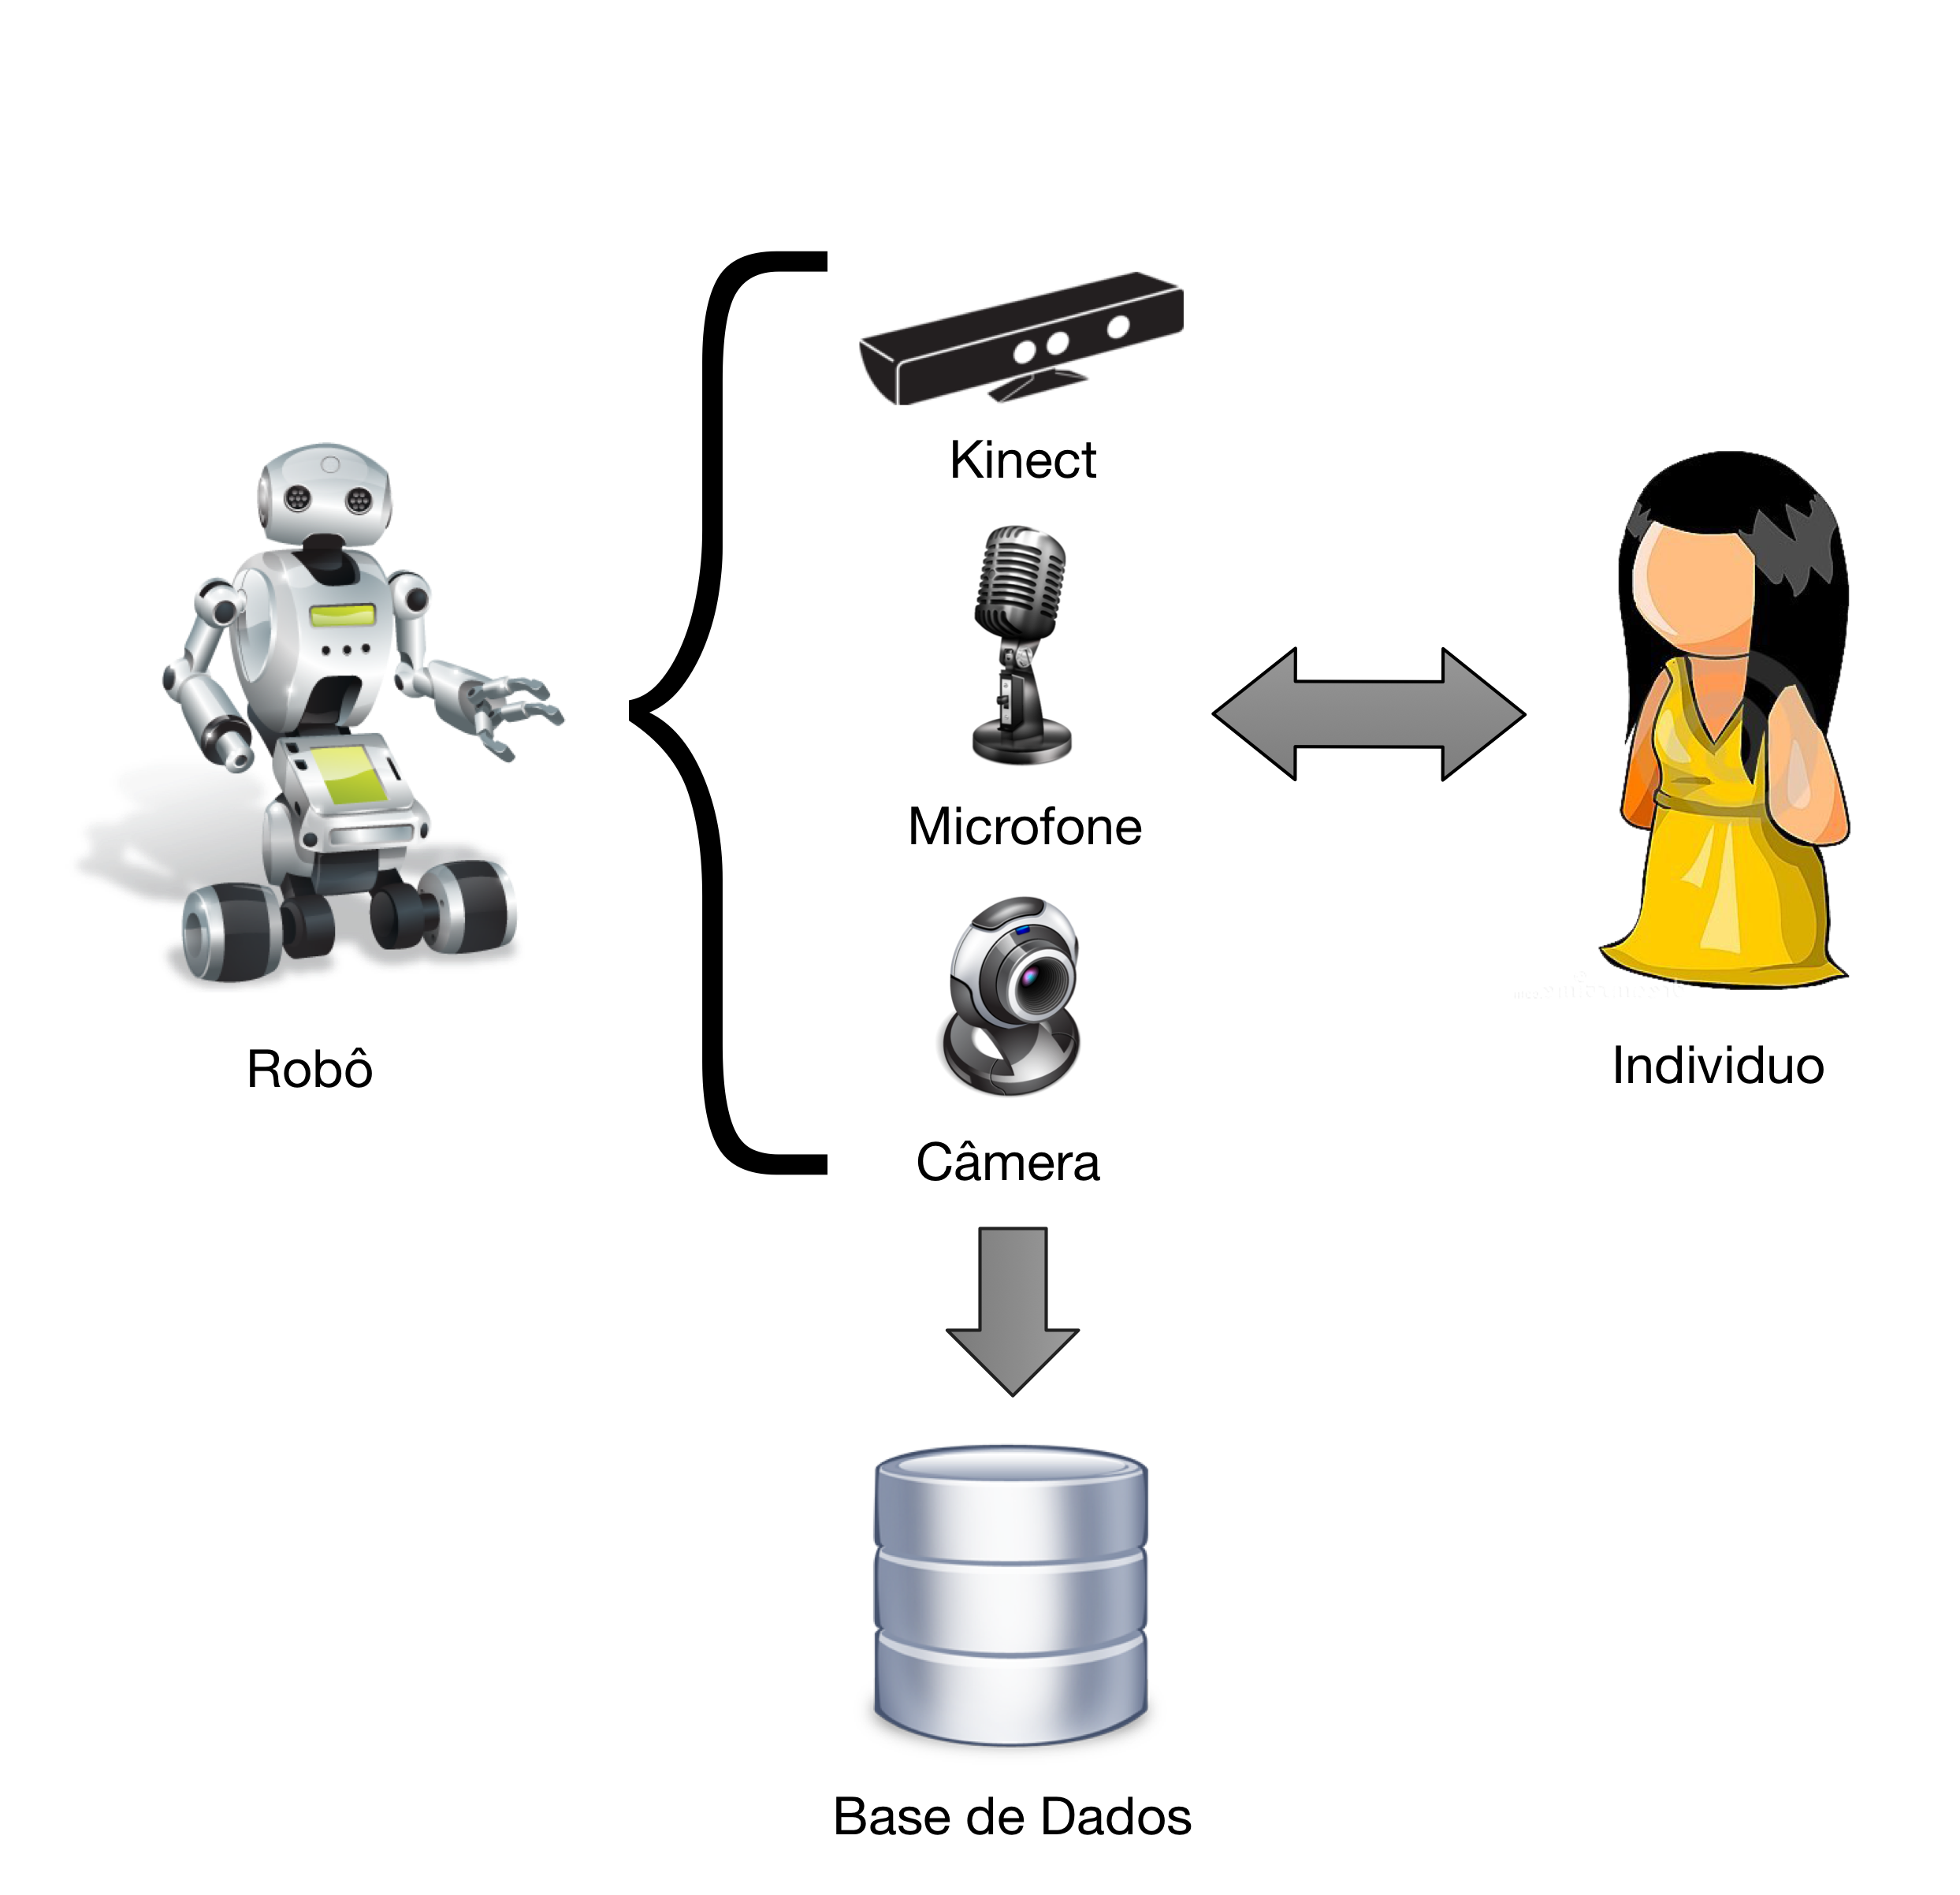
\includegraphics[scale=0.6]{images/captura_carac_individuo.png}
	\caption{Processo para a extração das características do individuo.}
	\label{fig:capturacaracteristicas}
\end{figure}

No processo apresentado pela figura \ref{fig:capturacaracteristicas}, o robô utiliza os sensores para identificar que o individuo iniciará uma interação com ele. Ao estabelecer o processo de interação, o robô utiliza um componente de \emph{log} que armazena todos os valores das variáveis que são utilizadas para determinar o perfil comportamental do individuo em um banco de dados. As variáveis são apresentadas em detalhes nas seções \ref{sec:variaveisindividuo} e \ref{sec:variaveisrobo}. Com as informações armazenadas determina-se através de um algoritmo de agrupamento, grupos que possuem perfis comportamentais similares, coletados e armazenados no banco de dados. Deve-se lembrar que as informações sobre o comportamento do individuo são direcionadas por um cenário de interação, como discutido por \citeonline{Jung:1991} em seu trabalho. 

Dessa forma, as variáveis aplicadas ao comportamento tem dependência do cenário de interação, porém as informações das variáveis etnográficas como idade, experiência computacional, sexo, local de origem, etnia, entre outras, são independentes do cenário. Existem alguns algoritmos na área de visão computacional que são capazes de identificar algumas variáveis etnográficas de maneira automática \cite{Yang:2007, Shan:2012, Ylioinas:2012, Samadi:2013, Amaral:2014}, porém para o trabalho desta tese, a coleta dessas informações será realizada através de um questionário pré interação já que esses algoritmos não fazem parte do objetivo principal do trabalho. As informações obtidas através do questionário serão inseridas no banco de dados complementando as informações de comportamento, que são separadas obtidas através da interação entre o ser humano e o robô através dos cenários de interação.

Na seção \ref{sec:variaveisindividuo} são detalhados os conjuntos de variáveis etnográficas e comportamentais com uma breve explicação dos objetivos esperados de cada uma das variáveis coletadas. A seção \ref{sec:variaveisrobo} detalha as variáveis que serão consideradas para o perfil do robô, apresentando também uma explicação sobre os objetivos de cada uma das variáveis.

\subsection{Selecionando as Variáveis para o Individuo}
\label{sec:variaveisindividuo}

Essa seção apresenta os conjuntos de variáveis que são consideradas nesse trabalho como a base de informações para seu desenvolvimento. Dois conjuntos são apresentados, o conjunto de variáveis etnográficas, seguido pelo conjunto de variáveis comportamentais que é o principal foco deste trabalho.

\subsubsection{Conjunto de Variáveis Etnográficas}
\label{sec:variaveisetnograficas}

O objetivo das variáveis etnográficas é identificar qual a experiência social e computacional de cada indivíduo. Além da experiência, também pode-se obter informações sobre a idade, gênero, local de nascimento ou origem do indivíduo. Todas essas informações são relevantes para verificar a existência de uma possível relação entre as variáveis etnográficas e comportamentais. A lista apresentada a seguir define as variáveis etnográficas e uma breve explicação sobre o significado de cada uma das variáveis.

\begin{enumerate}
	\item \textbf{Idade}: informa a idade do indivíduo.
	\item \textbf{Gênero}: informa o sexo biológico do indivíduo.
	\item \textbf{Local de Nascimento}: informa qual o local de nascimento do indivíduo. Essa variável auxiliará a determinar a base cultural do indivíduo.
	\item \textbf{Etnia}: informa a origem da família do indivíduo. Outra variável que auxilia na determinação da base cultural do indivíduo.
	\item \textbf{Quantidade de \emph{Gadgets}}: informa a quantidade de \emph{gadgets} que o indivíduo possui, ajudando a identificar qual a experiência e o contato dele com a tecnologia.
	\item \textbf{Contato prévio com Robôs}: informa apenas se o indivíduo já possuiu algum contato com robôs. Auxiliará a determinar o contato com a tecnologia, principalmente com robôs que poderá influenciar no seu comportamento durante a interação.
	\item \textbf{Tipos de Robôs}: informa quais são os tipos de robôs que o indivíduo teve contato. Os tipos poderão ser robôs \emph{Pet}, Humanoides, Androides, Móveis, entre outros. Essa variável é um complemento da variável ``Contato prévio com Robôs''.
	\item \textbf{Quantidade de cidades visitadas}: informa a quantidade de cidades que o indivíduo já visitou além da sua cidade natal. É importante para identificar o contato com outros tipos de cultura. Isso poderá influenciar no comportamento definido por sua cultura.
	\item \textbf{Quantidade de cidades que morou}: informa a quantidade de cidades que o indivíduo já morou além da sua cidade natal. É importante para identificar a vivência com outros tipos de cultura. Isso poderá influenciar no comportamento definido por sua cultura.
	\item \textbf{Quantidade de países visitadas}: informa a quantidade de países que o indivíduo já visitou além da sua cidade natal. É importante para identificar o contato com outros tipos de cultura. Isso poderá influenciar no comportamento definido por sua cultura.
	\item \textbf{Quantidade de países que morou}: informa a quantidade de países que o indivíduo já morou além da sua cidade natal. É importante para identificar a vivência com outros tipos de cultura. Isso poderá influenciar no comportamento definido por sua cultura.
\end{enumerate}

Em diversos trabalhos da seção \ref{sec:proxemicsihr}, onde a questão cultural do indivíduo é abordada, são discutidos que influência dela sobre o comportamenteo do o indivíduo. Contudo, a cultura é tratada como a origem do indivíduo, por exemplo, no trabalho de \citeonline{Eresha:2013}. Entretanto, a questão cultural na vida de uma pessoa é mais abrangente, está relacionada a experiência adquirida ao longo de sua vivência social. Dessa forma, o conjunto de variáveis apresentado acima tem como objetivo mapear de forma abstrata a experiência social do indivíduo, com o intuito de tornar o comportamento menos dependente da origem e talvez de sua experiência prévia.

Nesse trabalho, as informações levantadas nessa seção serão adquiridas através de questionários pré testes de interação. Em trabalhos futuros serão feitos estudos para identificar essas informações de maneira interativa através do próprio robô.

\subsubsection{Conjunto de Variáveis Comportamentais}
\label{sec:variaveiscomportamentais}

Variáveis comportamentais tem como principal objetivo identificar o comportamento do indivíduo. Nesse trabalho o comportamento está diretamente relacionado com cenários de interação social. As variáveis comportamentais são coletadas a partir de informações sobre as posições corporais e expressões faciais do indivíduo, tornando possível uma análise com base em teorias de linguagem corporal. As análises realizadas a partir da linguagem corporal, tem por base o trabalho apresentado por \citeonline{Lambert:2008}. O conjunto de variáveis comportamentais apresentados nessa seção não são utilizadas apenas para extrair o perfil do indivíduo, mas também para avaliar se a ação realizada pelo robô gerou uma reação positiva ou negativa no indivíduo. A lista apresentada a seguir define as variáveis comportamentais e uma breve explicação sobre o objetivo de cada uma das variáveis.

\begin{enumerate}
	\item \textbf{Expressões Faciais}: é possível identificar se a reação do indivíduo foi positiva ou negativa, a partir de uma ação do robô. Existem seis expressões bases que combinadas formam diversas outras~\cite{Bihan:2014}. Contudo, nesse trabalho será considerado apenas as seis expressões bases classificadas em dois grupos: expressões faciais positivas e expressões faciais negativas. O intuito dessa variável é realizar a avaliação da ação do robô com base nas expressões faciais do indivíduo.
	\item \textbf{Tempo de Transição entre as Zonas Sociais}: identificar o tempo que o indivíduo ficou confortável com a presença do robô a medida que esse diminuiu a distância entre eles.
	\item \textbf{Frequência do Olhar em direção ao Robô}: identificar se o indivíduo mantém o olhar ao robô, sendo possível saber se a interação está continua ou não. Isso pode influenciar se o robô está interagindo de maneira confortável ao indivíduo ou se esse está incomodado com a presença do robô.
	\item \textbf{Tempo do Olhar}: é possível mensurar o interesse do indivíduo durante a interação através do tempo que ele permanece com o olhar fixo no robô. Quanto maior o tempo do olhar, maior o interesse na interação do indivíduo.
	\item \textbf{Orientação dos ombros}: Auxilia a mensurar o interesse do indivíduo durante a interação, analisando se os ombros possuem a mesma orientação que a cabeça e também uma orientação em direção ao indivíduo que interage com o robô. Além disso, é possível determinar através do alinhamento do quadril com o ombro do indivíduo o ângulo de inclinação de seu torso. A inclinação do torso auxilia a identificar o interesse do indivíduo na interação, para isso basta verificar se ele está inclinado em direção ao robô para determinar um interesse positivo.
	\item \textbf{Orientação do quadril}: Auxilia a mensurar o interesse do indivíduo durante a interação. A orientação do quadril em direção ao robô ou na direção oposta auxilia a determinar o grau de interesse do indivíduo na interação. Quando mais alinhado à direção do robô, maior o interesse do indivíduo na interação.
	\item \textbf{Estilo da Voz}: é importante, pois pode determinar a reação que o indivíduo terá após a interação via áudio com o robô. Além disso, é possível determinar se o indivíduo está confortável ou não durante a interação, analisando o tom de sua voz ao responder o robô. Nesse trabalho, será considerado somente o canal de resposta ao indivíduo. A análise do tom da voz do indivíduo não será considerado nesta tese e ficará para trabalhos futuros de aprimoramento do componente de análise comportamental em IHR.
\end{enumerate}

\subsection{Selecionando as Variáveis para o Robô}
\label{sec:variaveisrobo}
Além das variáveis referentes ao perfil do indivíduo, deve-se considerar também as informações sobre o robô uma vez que sua aparência pode influenciar na reação das pessoas durante a interação~\cite{Hegel:2009}. Coletar as variáveis do robô pode auxiliar a identificar quais são os principais fatores que tornam a interação humano-robô desconfortável ou com menos qualidade. Dessa forma, foi definido um conjunto de variáveis que pudessem caracterizar da melhor maneira fatores do robô, referente a sua aparência, que influenciam na IHR. Esse conjunto de variáveis é apresentado a seguir:

\begin{enumerate}
	\item \textbf{Altura}: A altura do robô para identificar a influência da diferença entre alturas de robôs e humanos.
	\item \textbf{Volume}: O volume ocupado pelo robô pode influenciar no conforto da interação, uma vez que quando o robô atingir uma zona social mais próxima do indivíduo pode causar uma sensação claustrofóbica a ele.
	\item \textbf{Tipo do Robô}: Segundo \citeonline{Choi:2014}, robôs possuem dois tipos: Autônomos e Tele-operados. Essa variável define o quanto de intervenção humana é necessário para que o robô possa executar a tarefa objetivo.
	\item \textbf{Classificação do Robô}: Segundo \citeonline{Dobra:2014} classificar um robô é uma tarefa muito complexa e pode envolver diversas variáveis. Dessa forma, para essa tese será considerado uma classificação mais simples. O robô deve ser classificado como: fixo, móvel com rodas, móvel bípede, móvel quadrupede, móvel com manipuladores. Outras classificações podem ser inseridas conforme a necessidade e inclusão de novos robôs.
	\item \textbf{Aparência Física}: Essa variável descreve se o robô possui uma aparência amigável ou agressiva.
	\item \textbf{Nível de Ruído}: Determina qual o nível de ruído que os atuadores do robô podem gerar de tal forma, que possa influenciar na interação humano-robô.
\end{enumerate}

Além das variáveis que definem as características, é necessário também o mapeamento das ações que o robô irá executar para que exista uma avaliação dessa após a reação do indivíduo. As variáveis que compõem as informações do perfil comportamental do robô são:

\begin{enumerate}
	\item \textbf{Aproximação}: Forma de aproximação do robô ao indivíduo. Pode ser classificada entre rápida, devagar, brusca ou suave.
	\item \textbf{Movimentação do Manipulador}: Caso exista um manipulador deve descrever como é feita a movimentação do manipulador em direção ao usuário. A classificação consiste em brusca ou suave.
	\item \textbf{Estilo de Voz}: Ao emitir algum tipo de som o robô deverá manter um estilo de voz para que seja possível simbolizar qual o tipo de mensagem ele deseja falar. A classificação será feita de maneira simplificada, considerando apenas se é um estilo educado ou agressivo.
	\item \textbf{Expressão Facial}: Ao iniciar o contato visual com o indivíduo, pode ocorrer diversas expressões do robô na tentativa de manter o conforto do indivíduo durante o processo de interação. Simplificando as expressões, de maneira similar ao apresentado na seção~\ref{sec:variaveiscomportamentais}, são consideradas apenas dois tipos de expressões realizadas pelo robô: amistoso e não-amistoso. As expressões faciais do robô serão executadas através do \emph{tablet} acoplado nele, conforme descrito na seção~\ref{sec:robo}.
\end{enumerate}

As variáveis comportamentais do robô definidas com o objetivo de executar uma tarefa de abordagem para estabelecer uma interação. Caso seja necessário adicionar novas variáveis a esse conjunto não haverá problema ao método apresentado ao longo da seção.

\section{Raciocinando com Base nas Interações Extraídas}
\label{sec:raciociniointeracao}

Com as variáveis comportamentais e etnográficas do indivíduo e do robô definidas é necessário definir o método que fará com que o robô seja capaz de aprender a interagir com seres humanos a partir das suas experiências passadas. No capitulo \ref{cap:rbc} foi apresentado a técnica de Raciocínio Baseado em Casos (RBC) que tem como principal objetivo o desenvolvimento de um sistema de conhecimento com base em experiências ou casos ocorridos anteriormente. RBC tem uma estrutura baseada em 4(quatro) pilares, são eles~\cite{Lopez:2013}: Resgatar, Reutilizar, Revisar e Reter. A figura~\ref{fig:rbc} apresenta a metodologia dessa tese, que engloba as quatro etapas do RBC.

\begin{figure}[ht!]
	\centering
	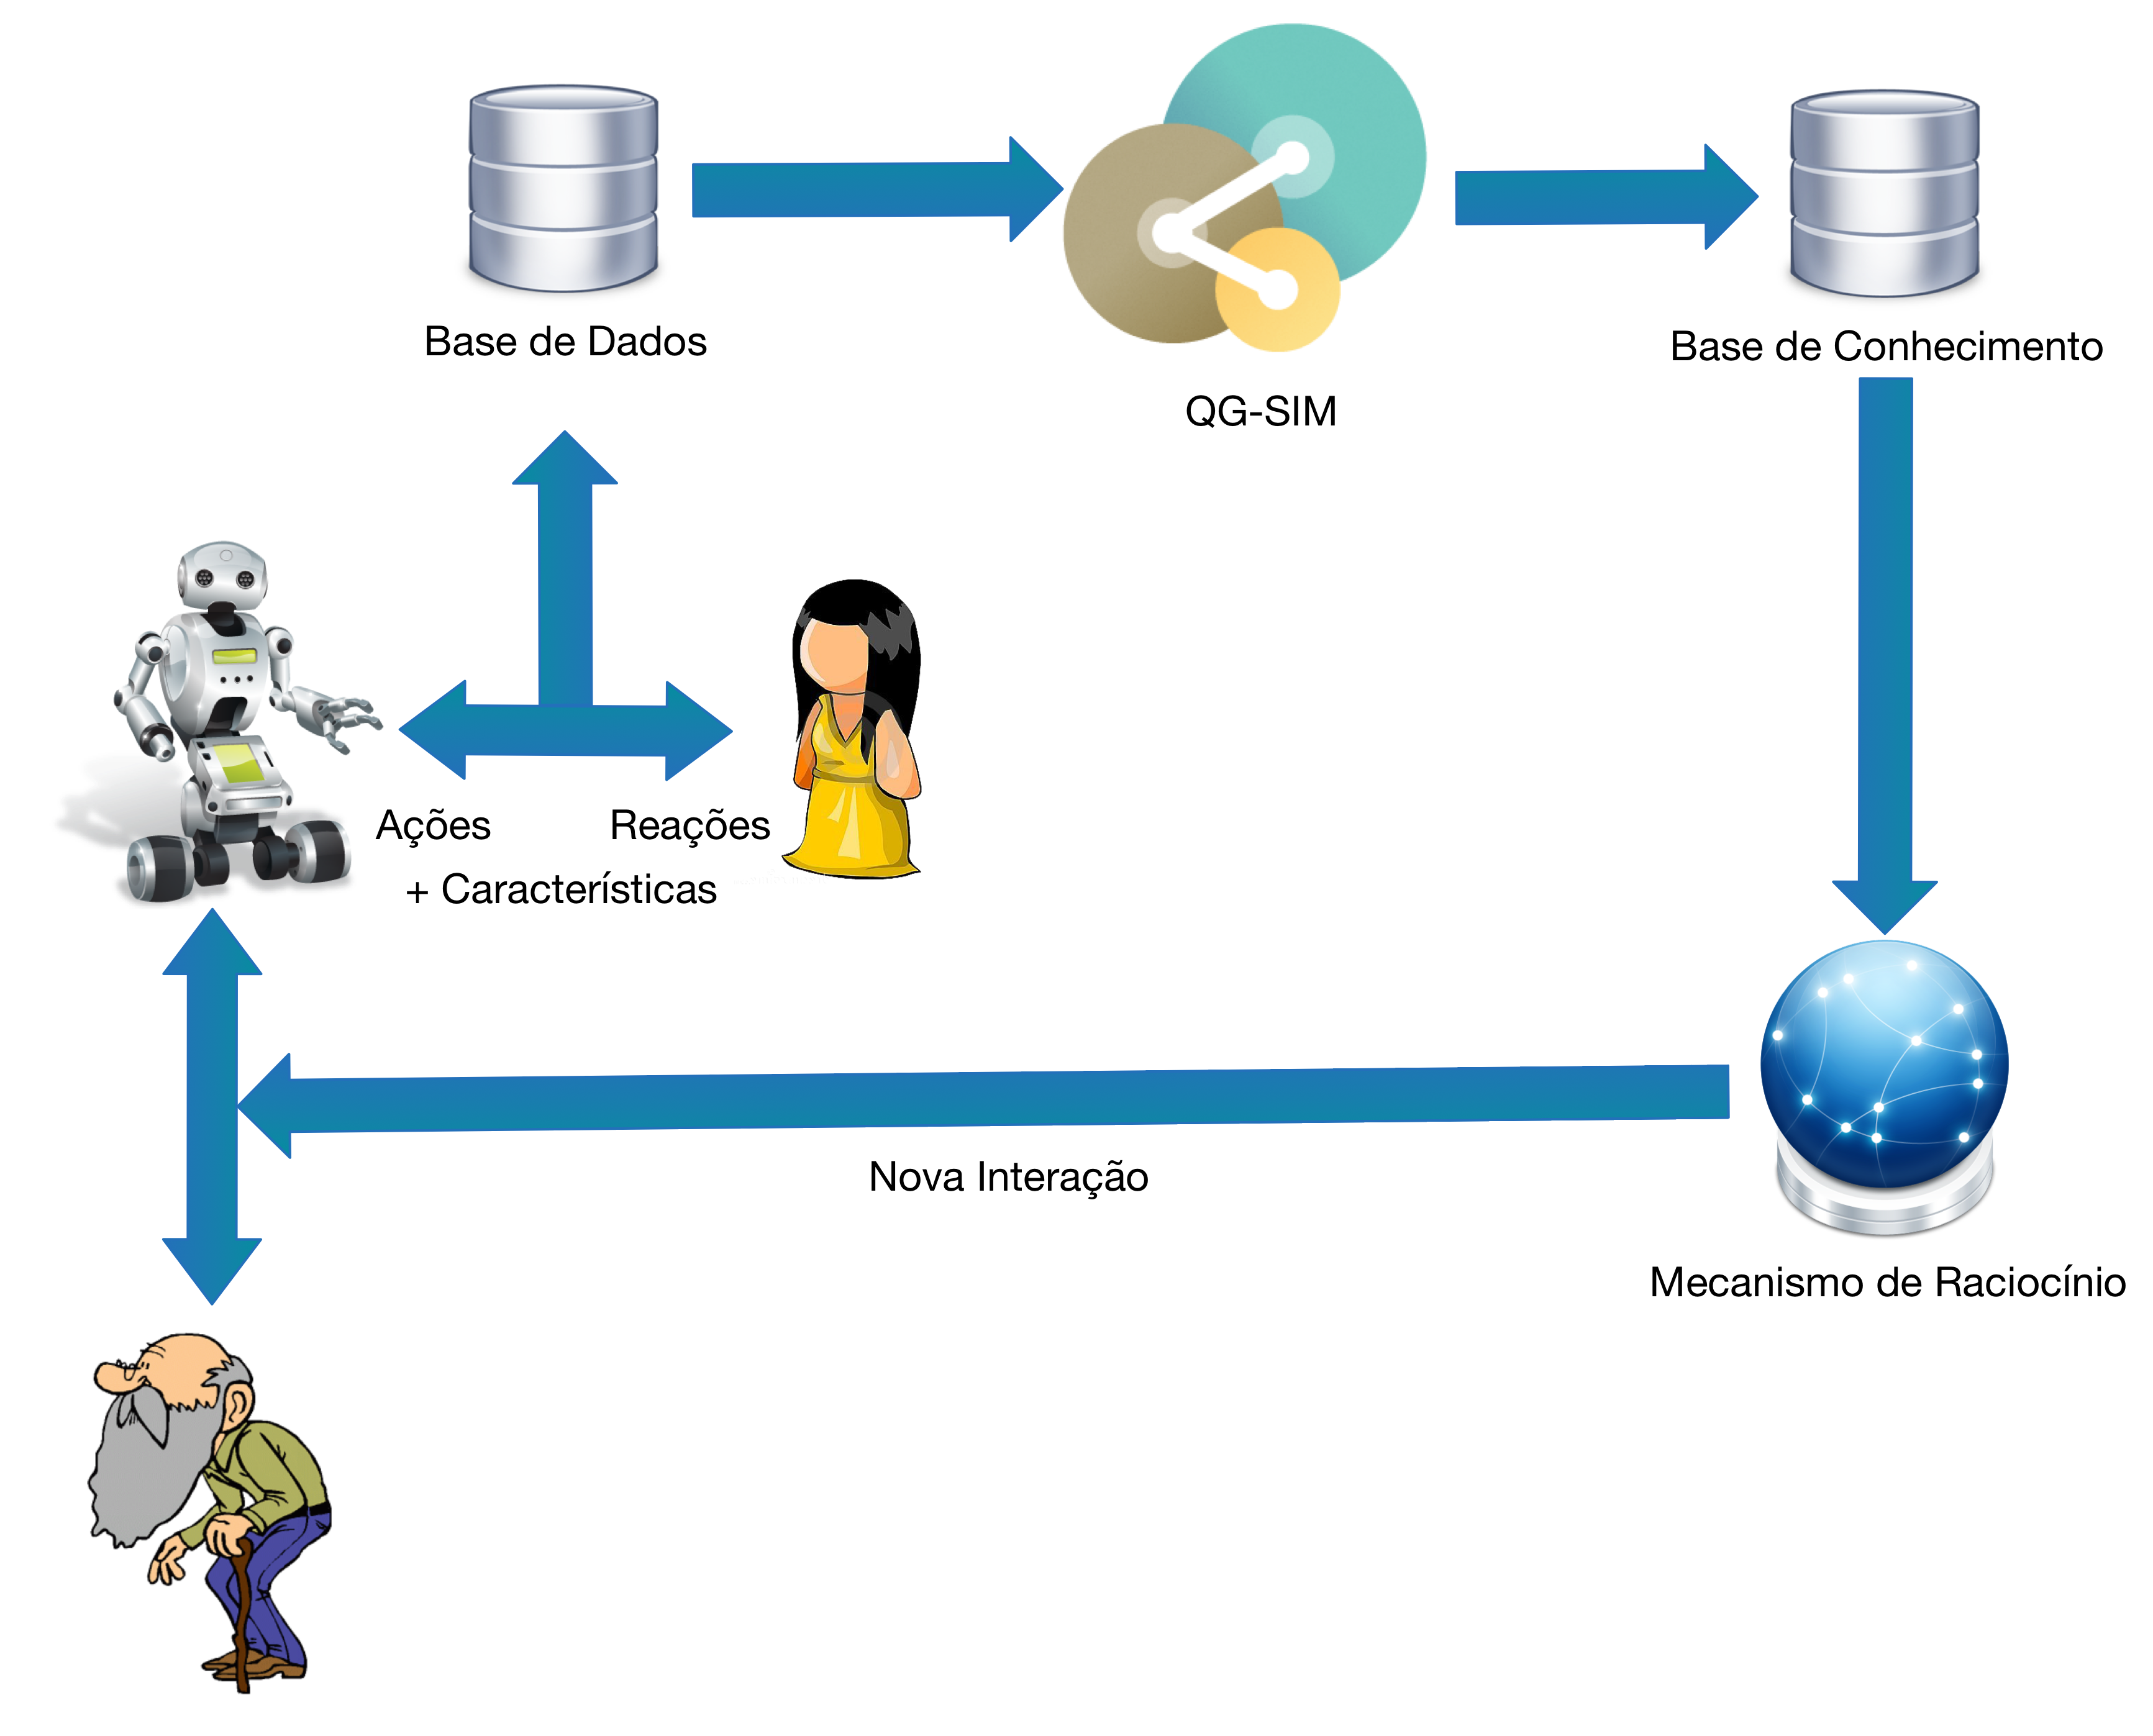
\includegraphics[width=\textwidth]{images/rbc_geral.png}
	\caption{Processo de Interação com Aprendizado baseado em Experiências Passadas.}
	\label{fig:rbc}
\end{figure}

A metodologia da figura~\ref{fig:rbc} tem início na interação entre o robô e a jovem localizada a sua frente. Durante a interação entre os dois o sistema coleta todas as reações da jovem para cada ação tomada pelo robô, de acordo com as variáveis descritas na seção~\ref{sec:extracaocaracteristicas}, que são armazenadas na base de dados. A base de dados formada a partir dessas informações é enviada ao algoritmo de agrupamento por similaridade QG-SIM (Quality Groups of Similarity, em inglês)~\cite{Masiero:2013}. Os grupos gerados pelo QG-SIM são analisados e inseridos na base de conhecimento formando os casos de pesquisa para novas interações. Quando ocorrer uma nova interação, como por exemplo o robô com o senhor na figura~\ref{fig:rbc}, o mecanismo de raciocínio realiza uma análise para que possa inferir qual o melhor caso a ser aplicado para interação entre o senhor e o robô. Mesmo que utilize casos existentes na base de conhecimento, todas as interações são armazenadas para manter o aprendizado sobre interações contínuo e sempre com o objetivo de manter o individuo confortável durante todo o processo. Na sequência serão detalhadas as fases do RBC de acordo com a metodologia apresentada na figura~\ref{fig:rbc}.

\subsection{Resgatar}
\label{sec:resgatar}

A partir de uma nova interação inicia-se o processo de resgate do caso que maximize as reações positivas de um determinado indivíduo a partir da ação que o robô realiza. Nessa fase a solução encontrada não poderá ser dada como exclusiva, pois quando trata-se de seres humanos a tarefa de determinar uma solução exata é complexa. Como para um mesmo perfil de indivíduo ou um perfil similar pode-se apresentar muitas soluções deve ser aplicado nessa fase um modelo probabilístico de tal forma, que a solução escolhida seja a que possui um maior valor de probabilidade no ponto de vista de maximizar a satisfação e o conforto do indivíduo.

Existem diversos métodos probabilísticos que podem ser aplicados nessa fase, como por exemplo, redes Bayesianas ou até mesmo conjunto de lógica nebulosa (Lógica \emph{Fuzzy}). Mesmo sendo o regaste de uma solução único para o caso, esse modelo possibilita que a solução selecionada para execução seja a melhor dentre todas as armazenadas dada uma distribuição probabilística. Selecionando o caso que será aplicado esse deve formar um conjunto de ações do robô para interação com o indivíduo, como é apresentado na próxima seção.

\subsection{Reutilizar}
\label{sec:reutilizar}

Após o resgate do caso que possui a maior similaridade de tornar a interação confortável ao indivíduo é necessário construir a sequência de ações que o robô irá executar. Para isso, deve-se considerar duas premissas. A primeira é que uma ação é dependente da anterior, pois caso essa premissa não seja considerada as ações que o robô executará não apresentarão nenhum sentido ao indivíduo. Isso faz com que esse modelo de reutilização seja considerado como temporal, onde uma ação futura depende de uma ação passada. A segundo premissa que deve ser considerada é que o indivíduo irá se comportar de maneira diferente da esperada em algum momento do processo de interação. Dessa maneira, deve-se realizar um novo resgate para a solução que maximiza o conforto da interação a partir daquele ponto onde a reação do indivíduo foi diferente do esperado.

\subsection{Reter}
\label{sec:reter}

Durante a interação entre o robô e um indivíduo as informações sobre o comportamento são armazenadas em um banco de dados. A partir desse banco de dados é realizado um agrupamento entre os perfis comportamentais que possuem uma certa similaridade. Para realizar esse agrupamento é utilizado um algoritmo chamado QG-SIM. O QG-SIM~\cite{Masiero:2013} mantém a qualidade da similaridade entre os perfis de um mesmo grupo, sendo dessa maneira, o algoritmo ideal para esse tipo de tarefa e cenário.

Com os grupos formados é utilizado uma processo definido por \citeonline{Masiero:2013} para gerar um perfil comum ao grupo. Esse perfil comum também pode ser considerado a centroide do grupo. O procedimento para encontrar a centroide do grupo auxilia a determinar o perfil que será inserido na base do conhecimento que é utilizada no processo de resgate e reutilização do sistema de RBC.

A opção de realizar esse processo de agrupamento para inserir um caso na base de conhecimento é importante, pois diminui a quantidade de casos para busca por parte do sistema de RBC. Diminuir o número de casos aumenta o desempenho do algoritmo fazendo com que o robô tenha uma resposta na interação mais rápida, evitando com que o indivíduo espere muito por uma ação do robô.

\subsection{Revisar}
\label{sec:revisar}

Com a base de conhecimento formada é executado um procedimento para verificar se existem perfis iguais ou similares a ponto que possam ser excluídos. Dessa maneira, é possível manter a base de conhecimento sempre com perfis exclusivos entre os existentes. Assim, é possível garantir que um número maior de indivíduos seja atendido pelo sistema de RBC.

Apesar da metodologia apresentada na figura~\ref{fig:rbc} possuir apenas um robô na interação, é possível transferir esse conhecimento a diversos robôs já que em sua arquitetura todo o sistema de RBC é extra robô. Assim, o processamento e conhecimento adquirido pelo sistema de RBC ficará disponível em um servidor ao qual todo robô que quiser utilizar dessas informações terá livre acesso.

Todo esse sistema será testado em um cenário de primeiro contato para interação entre dois agentes, nesse caso um robô e um indivíduo. O robô utilizado tem a locomoção feita através de rodas, porém sua altura é próxima da média dos seres humanos. As características do robô fazem com que ele seja apropriado para interações entre humanos e robôs.
%!TEX root=Principal.tex
\chapter{RESULTADOS E DISCUSSÕES}
\label{cap:resultados}
Ao total foram realizados 55 testes com usuários interagindo com o robô em ambiente doméstico. Os testes ocorreram de acordo com o cenrário do contexto de uso apresentado na figura~\ref{fig:contextouso}. Dos 55 participantes 39 foram selecionados para realizar o teste inicial que foi base para criação do classificador bayesiano. Outros 16 são utilizados para validação e mensurar o acerto do classificador. Os perfis dos usuários selecionados atendem o escopo do projeto enviado do comitê de ética sobre o registro CAAE: 70057117.0.0000.5508. A tabela~\ref{tab:perfilamostra} apresenta as informações básicas sobre os usuários selecionados para realizar os testes iniciais.

\begin{table}[!ht]
	\caption{Perfis dos 39 usuários que realizaram o teste inicial.}
	\label{tab:perfilamostra}
	\centering
	\begin{tabular}{c | c | c | c | c | c | c | c}
        \hline
        Idade & Altura & Gênero & Feição & Sociável? & Óculos & Cabelo & Etnia \\
         &  &  &  &  & de Grau? & Comprido? &  \\ \hline
        31 & 1.74 & Masculino & Normal & Sim & Não & Não & Branca \\ \hline
        24 & 1.80 & Masculino & Sorridente & Sim & Sim & Não & Branca \\ \hline
        26 & 1.70 & Masculino & Sorridente & Sim & Não & Não & Parda \\ \hline
        19 & 1.70 & Masculino & Normal & Não & Não & Não & Branca \\ \hline
        20 & 1.68 & Feminino  & Sorridente & Sim & Sim & Sim & Branca \\ \hline
        20 & 1.63 & Feminino  & Normal & Sim & Sim & Não & Parda \\ \hline
        20 & 1.68 & Masculino & Sorridente & Sim & Sim & Não & Branca \\ \hline
        20 & 1.80 & Masculino & Sorridente & Sim & Sim & Não & Branca \\ \hline
        34 & 1.85 & Masculino & Normal & Sim & Não & Não & Branca \\ \hline
        22 & 1.61 & Feminino  & Séria/Fechada & Sim & Sim & Sim & Preta \\ \hline
        23 & 1.80 & Masculino & Séria/Fechada & Não & Sim & Não & Branca \\ \hline
        20 & 1.65 & Masculino & Sorridente & Sim & Sim & Não & Branca \\ \hline
        24 & 1.68 & Masculino & Séria/Fechada & Sim & Não & Não & Branca \\ \hline
        20 & 1.75 & Masculino & Sorridente & Não & Sim & Não & Branca \\ \hline
        21 & 1.80 & Masculino & Normal & Não & Não & Não & Branca \\ \hline
        22 & 1.72 & Masculino & Sorridente & Sim & Sim & Não & Branca \\ \hline
        26 & 1.75 & Masculino & Sorridente & Sim & Não & Não & Branca \\ \hline
        30 & 1.59 & Feminino  & Normal & Sim & Não & Sim & Parda \\ \hline
        27 & 1.83 & Masculino & Normal & Sim & Não & Não & Parda \\ \hline
        24 & 1.78 & Masculino & Normal & Sim & Não & Não & Preta \\ \hline
        42 & 1.78 & Masculino & Sorridente & Sim & Não & Sim & Branca \\ \hline
        33 & 1.85 & Masculino & Sorridente & Sim & Sim & Não & Branca \\ \hline
        24 & 1.70 & Masculino & Normal & Sim & Não & Não & Branca \\ \hline
        24 & 1.76 & Masculino & Normal & Sim & Não & Não & Branca \\ \hline
        18 & 1.63 & Masculino & Sorridente & Sim & Sim & Sim & Branca \\ \hline
        33 & 1.75 & Masculino & Sorridente & Sim & Não & Não & Branca \\ \hline
        22 & 1.67 & Feminino  & Sorridente & Sim & Não & Não & Branca \\ \hline
        22 & 1.67 & Masculino & Séria/Fechada & Sim & Não & Não & Preta \\ \hline
        21 & 1.51 & Feminino  & Normal & Não & Sim & Sim & Amarela \\ \hline
        19 & 1.73 & Masculino & Normal & Sim & Não & Não & Branca \\ \hline
        34 & 1.66 & Feminino  & Sorridente & Não & Sim & Sim & Amarela \\ \hline
        39 & 1.77 & Masculino & Normal & Sim & Não & Não & Branca \\ \hline
        22 & 1.63 & Feminino  & Normal & Sim & Não & Sim & Branca \\ \hline
        19 & 1.80 & Masculino & Sorridente & Não & Não & Não & Branca \\ \hline
        20 & 1.75 & Masculino & Normal & Sim & Não & Não & Branca \\ \hline
        36 & 1.68 & Feminino  & Normal & Sim & Não & Não & Branca \\ \hline
        20 & 1.87 & Masculino & Normal & Sim & Sim & Não & Branca \\ \hline
        40 & 1.74 & Feminino  & Normal & Sim & Sim & Não & Branca \\ \hline
        23 & 1.82 & Masculino & Normal & Sim & Não & Não & Branca \\ \hline
	\end{tabular}
	\smallcaption{Fonte: O autor.}
\end{table}

A tabela~\ref{tab:perfilamostra} apresenta as informações declaradas sobre todos os paritipantes do teste de para criação do classificador. Pode-se identificar os limites das variáveis dos parcipantes como, a idade mínima apresentada é de 18 anos e a máxima de 42 anos. A relação entre altura das pessoas, a menor estatura foi de 1,51 m contra 1,87 m da maior. Foram 29 homens e 10 mulheres na amostra, distribuídos entre funcionários e alunos da instituição de ensino. As informações apresentadas na tabela~\ref{tab:perfilamostra} são referentes as características etnográficas e algumas tem relação ao comportamento do usuário, como no caso de feição e se o usuário é sociável. Elas auxiliam na construção do perfil etnográfico do usuário. Todas essas informações obtidas através do questionário pré experimento são confrontadas com as informações do pós para análise.

Durante os testes iniciais, com os 39 participantes, o foco foi entender como eles se sentiam em um cenário de interação doméstico enquanto o robô se aproximava e executava algumas ações. O sentimento durante a interação foi traduzido em conforto e medo, através do questionário pós teste. Confrontando algumas informações, foram gerados alguns gráficos que auxiliam na visualização do perfil dos usuários que participaram do teste.

A figura~\ref{fig:confortogenero} apresenta a relação das informações sobre gênero dos participantes e o quanto ele se sentiu confortável na interação com o robô sendo o menor valor para totalmente desconfortável e o maior totalmente confortável.

\begin{figure}[ht!]
	\centering
	\begin{minipage}{0.65\textwidth}
		\caption{Conforto por gênero.}
		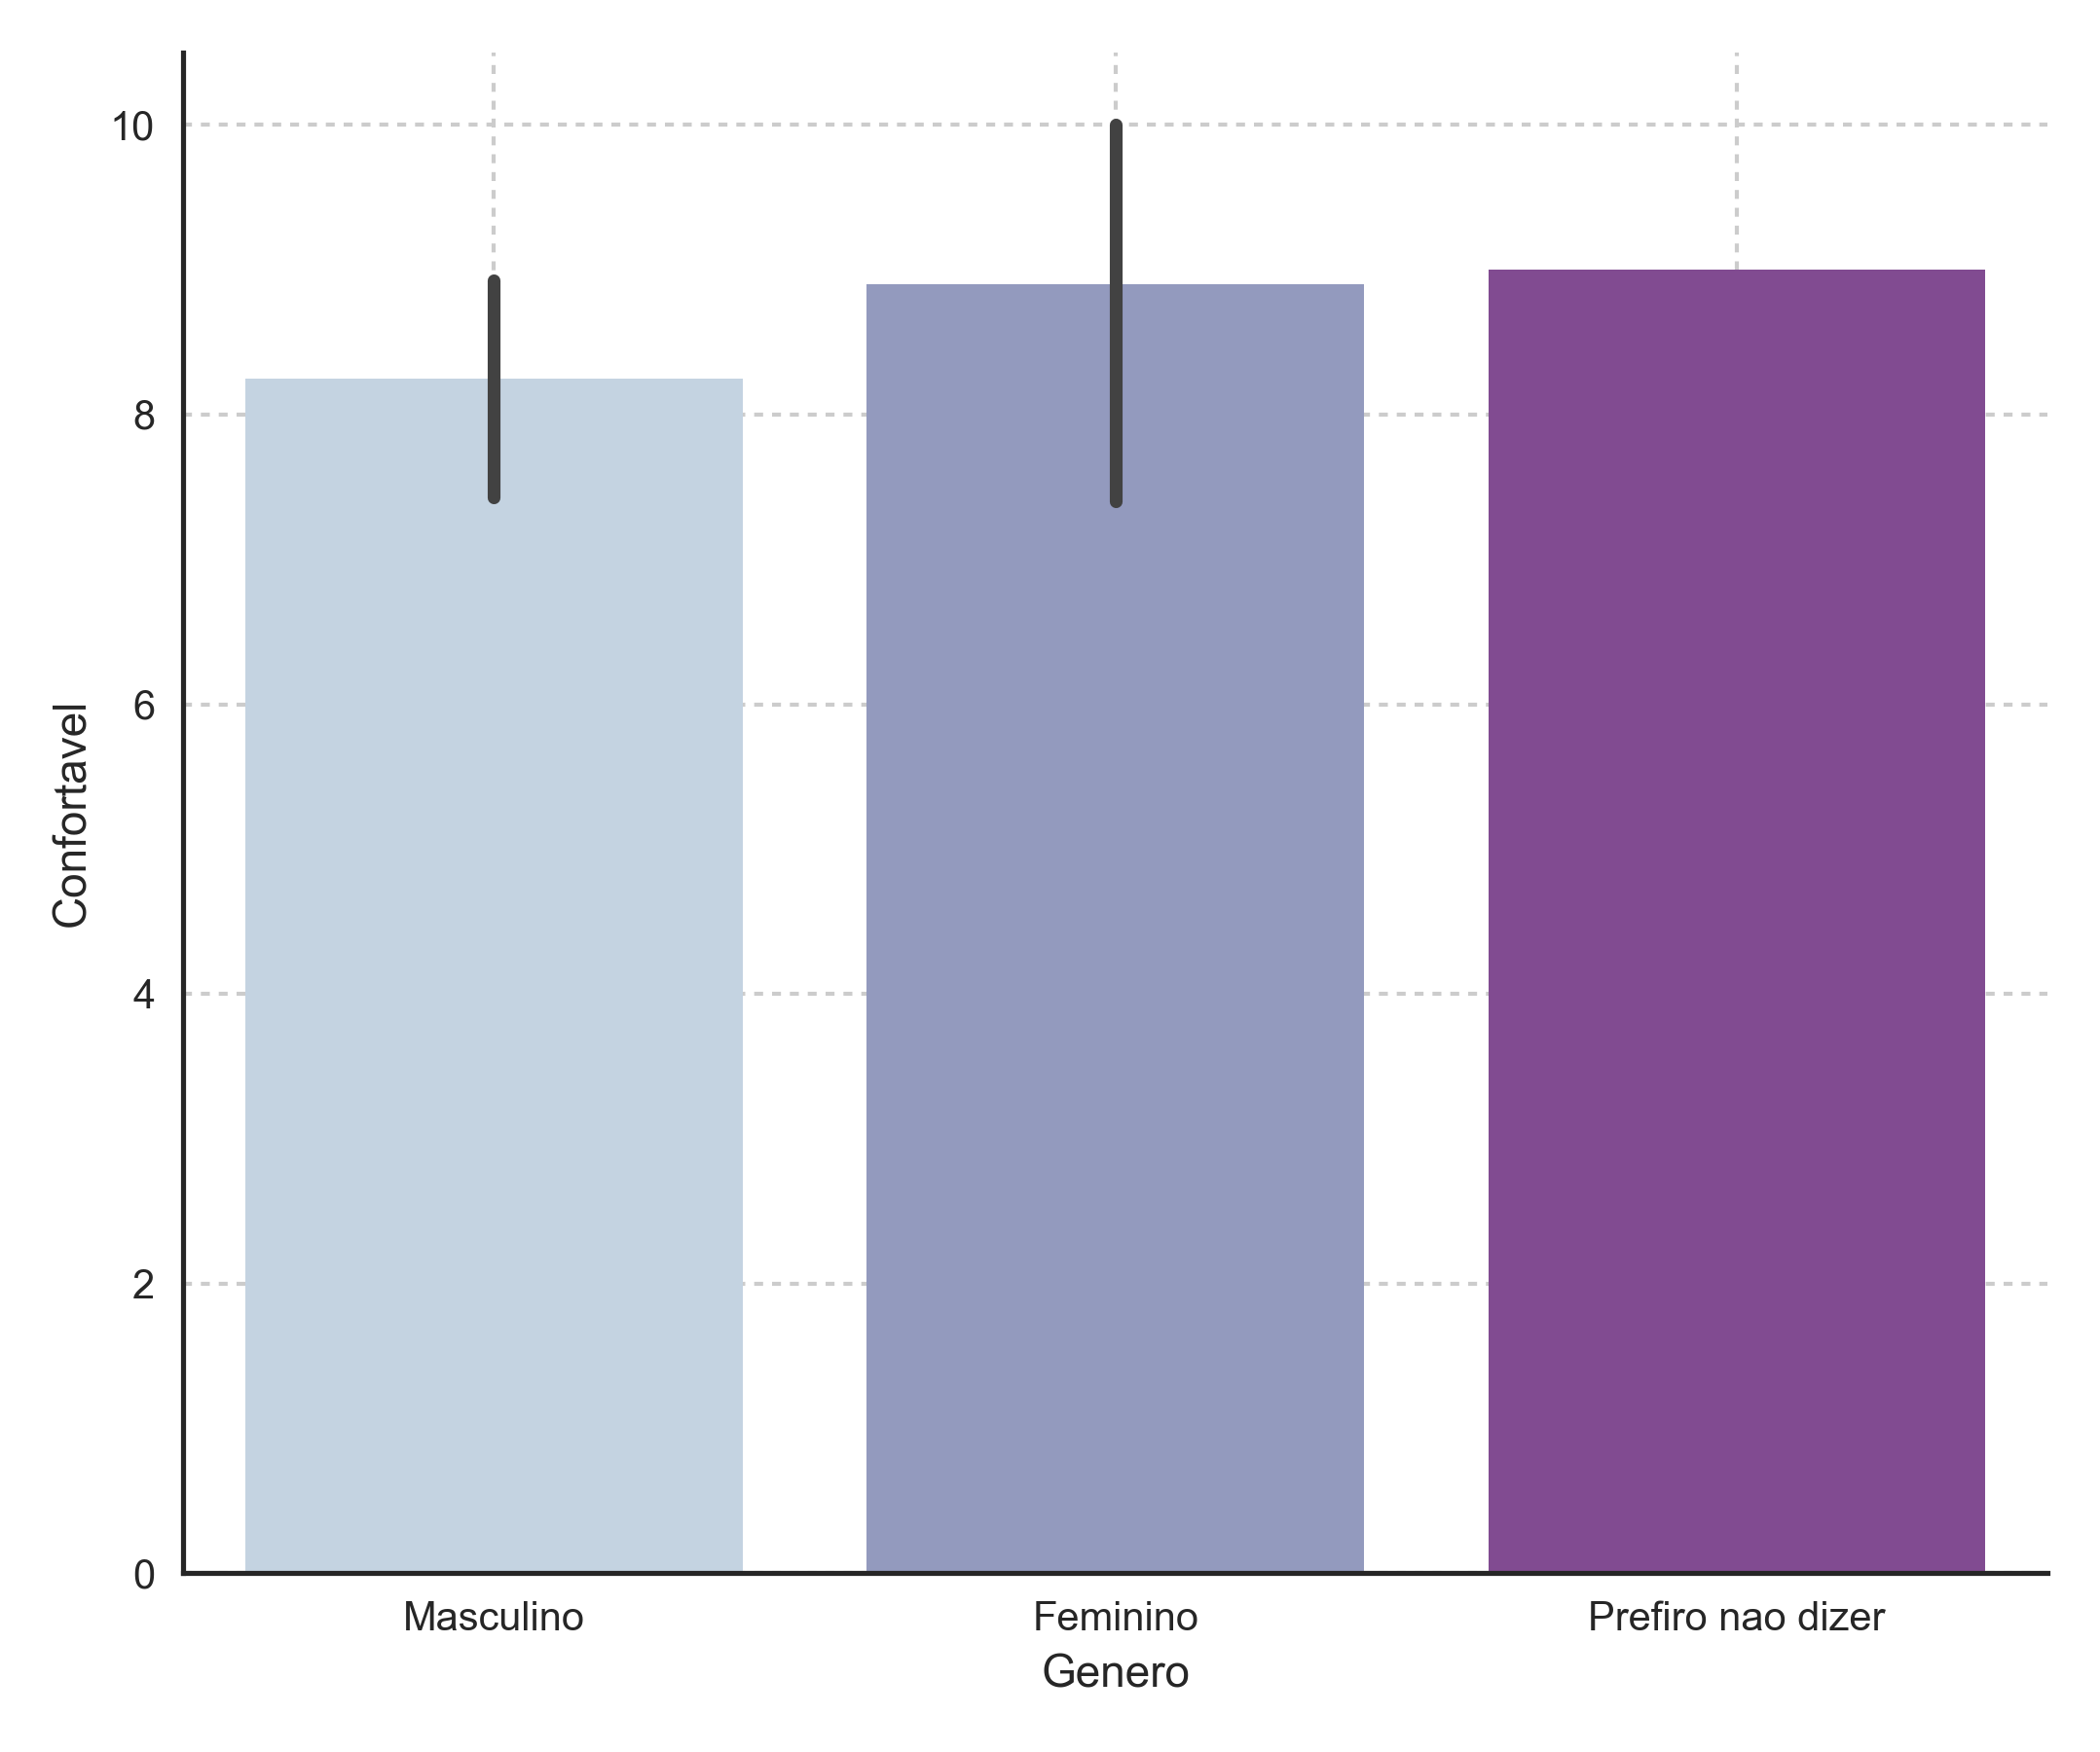
\includegraphics[width=\textwidth]{conforto_genero.png}
		\smallcaption{Fonte: O autor.}
		\label{fig:confortogenero}
	\end{minipage}
\end{figure}

Pode-se observar na figura~\ref{fig:confortogenero} que houve um equilíbrio entre os gêneros com relação ao conforto na aproximação do robô. Na média os homens ficaram 8.25 confortável na escala Likert, com o desvio padrão de 1.9933. As mulheres tiveram a média 8.9 e o desvio padrão em 2.0224. Isso ocorreu em grande parte devido a exibição das expressões faciais do robô. Os participantes do gênero feminino acolheram o robô como uma criança ou pessoa meiga se aproximando dela. Outra variável que é comparada é a idade dos partipantes com o nível de conforto, apresentado na figura~\ref{fig:confortoidade}.

\begin{figure}[ht!]
	\centering
	\begin{minipage}{0.65\textwidth}
		\caption{Conforto por idade.}
		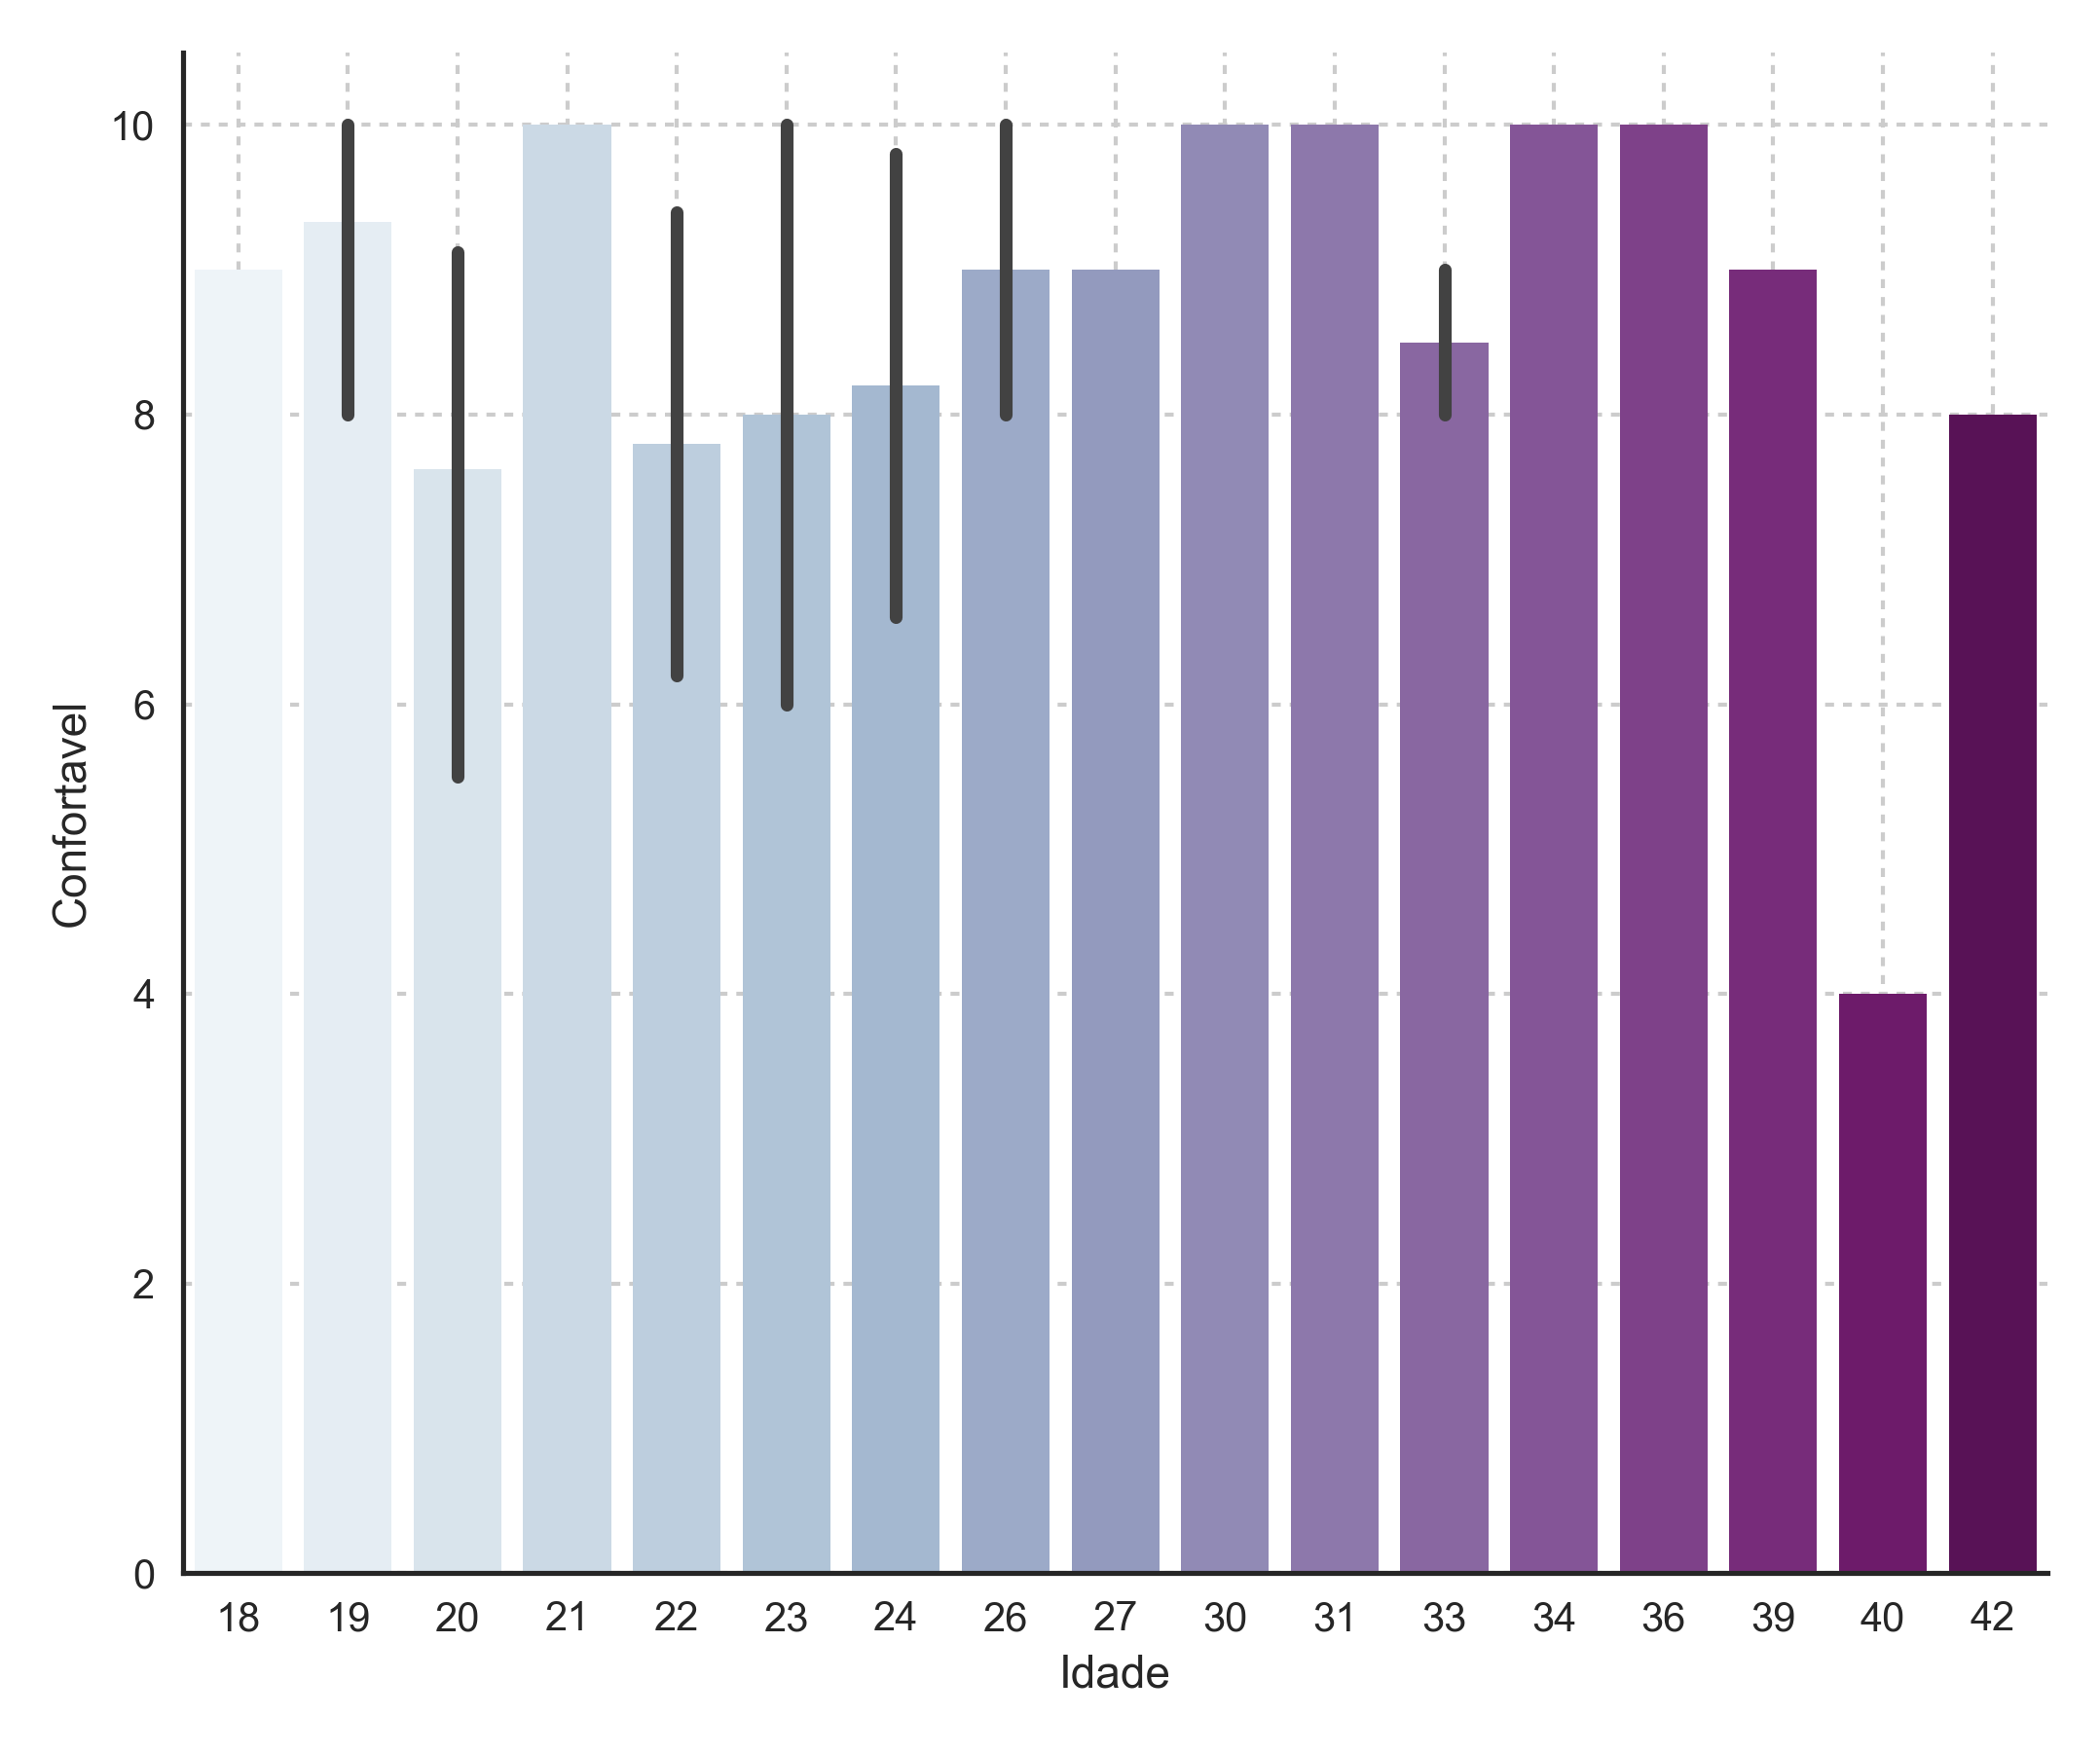
\includegraphics[width=\textwidth]{conforto_idade.png}
		\smallcaption{Fonte: O autor.}
		\label{fig:confortoidade}
	\end{minipage}
\end{figure}

Dois participantes apresentaram um nível de desconforto, mais elevado que os demais participantes, na aproximação do robô. Um participante apresentou a idade de 20 anos e outro de 40 anos. Foram os que ficaram mais desconfortáveis com o robô, como observado na figura~\ref{fig:confortoidade}. Os demais demonstraram-se confortavéis com o robô na aproximação.

Na figura~\ref{fig:confortoposicao} é apresentada a relação entre o conforto do participante e a posição dele durante a interação, sentado ou em pé.

\begin{figure}[ht!]
	\centering
	\begin{minipage}{0.65\textwidth}
		\caption{Conforto por posição de interação.}
		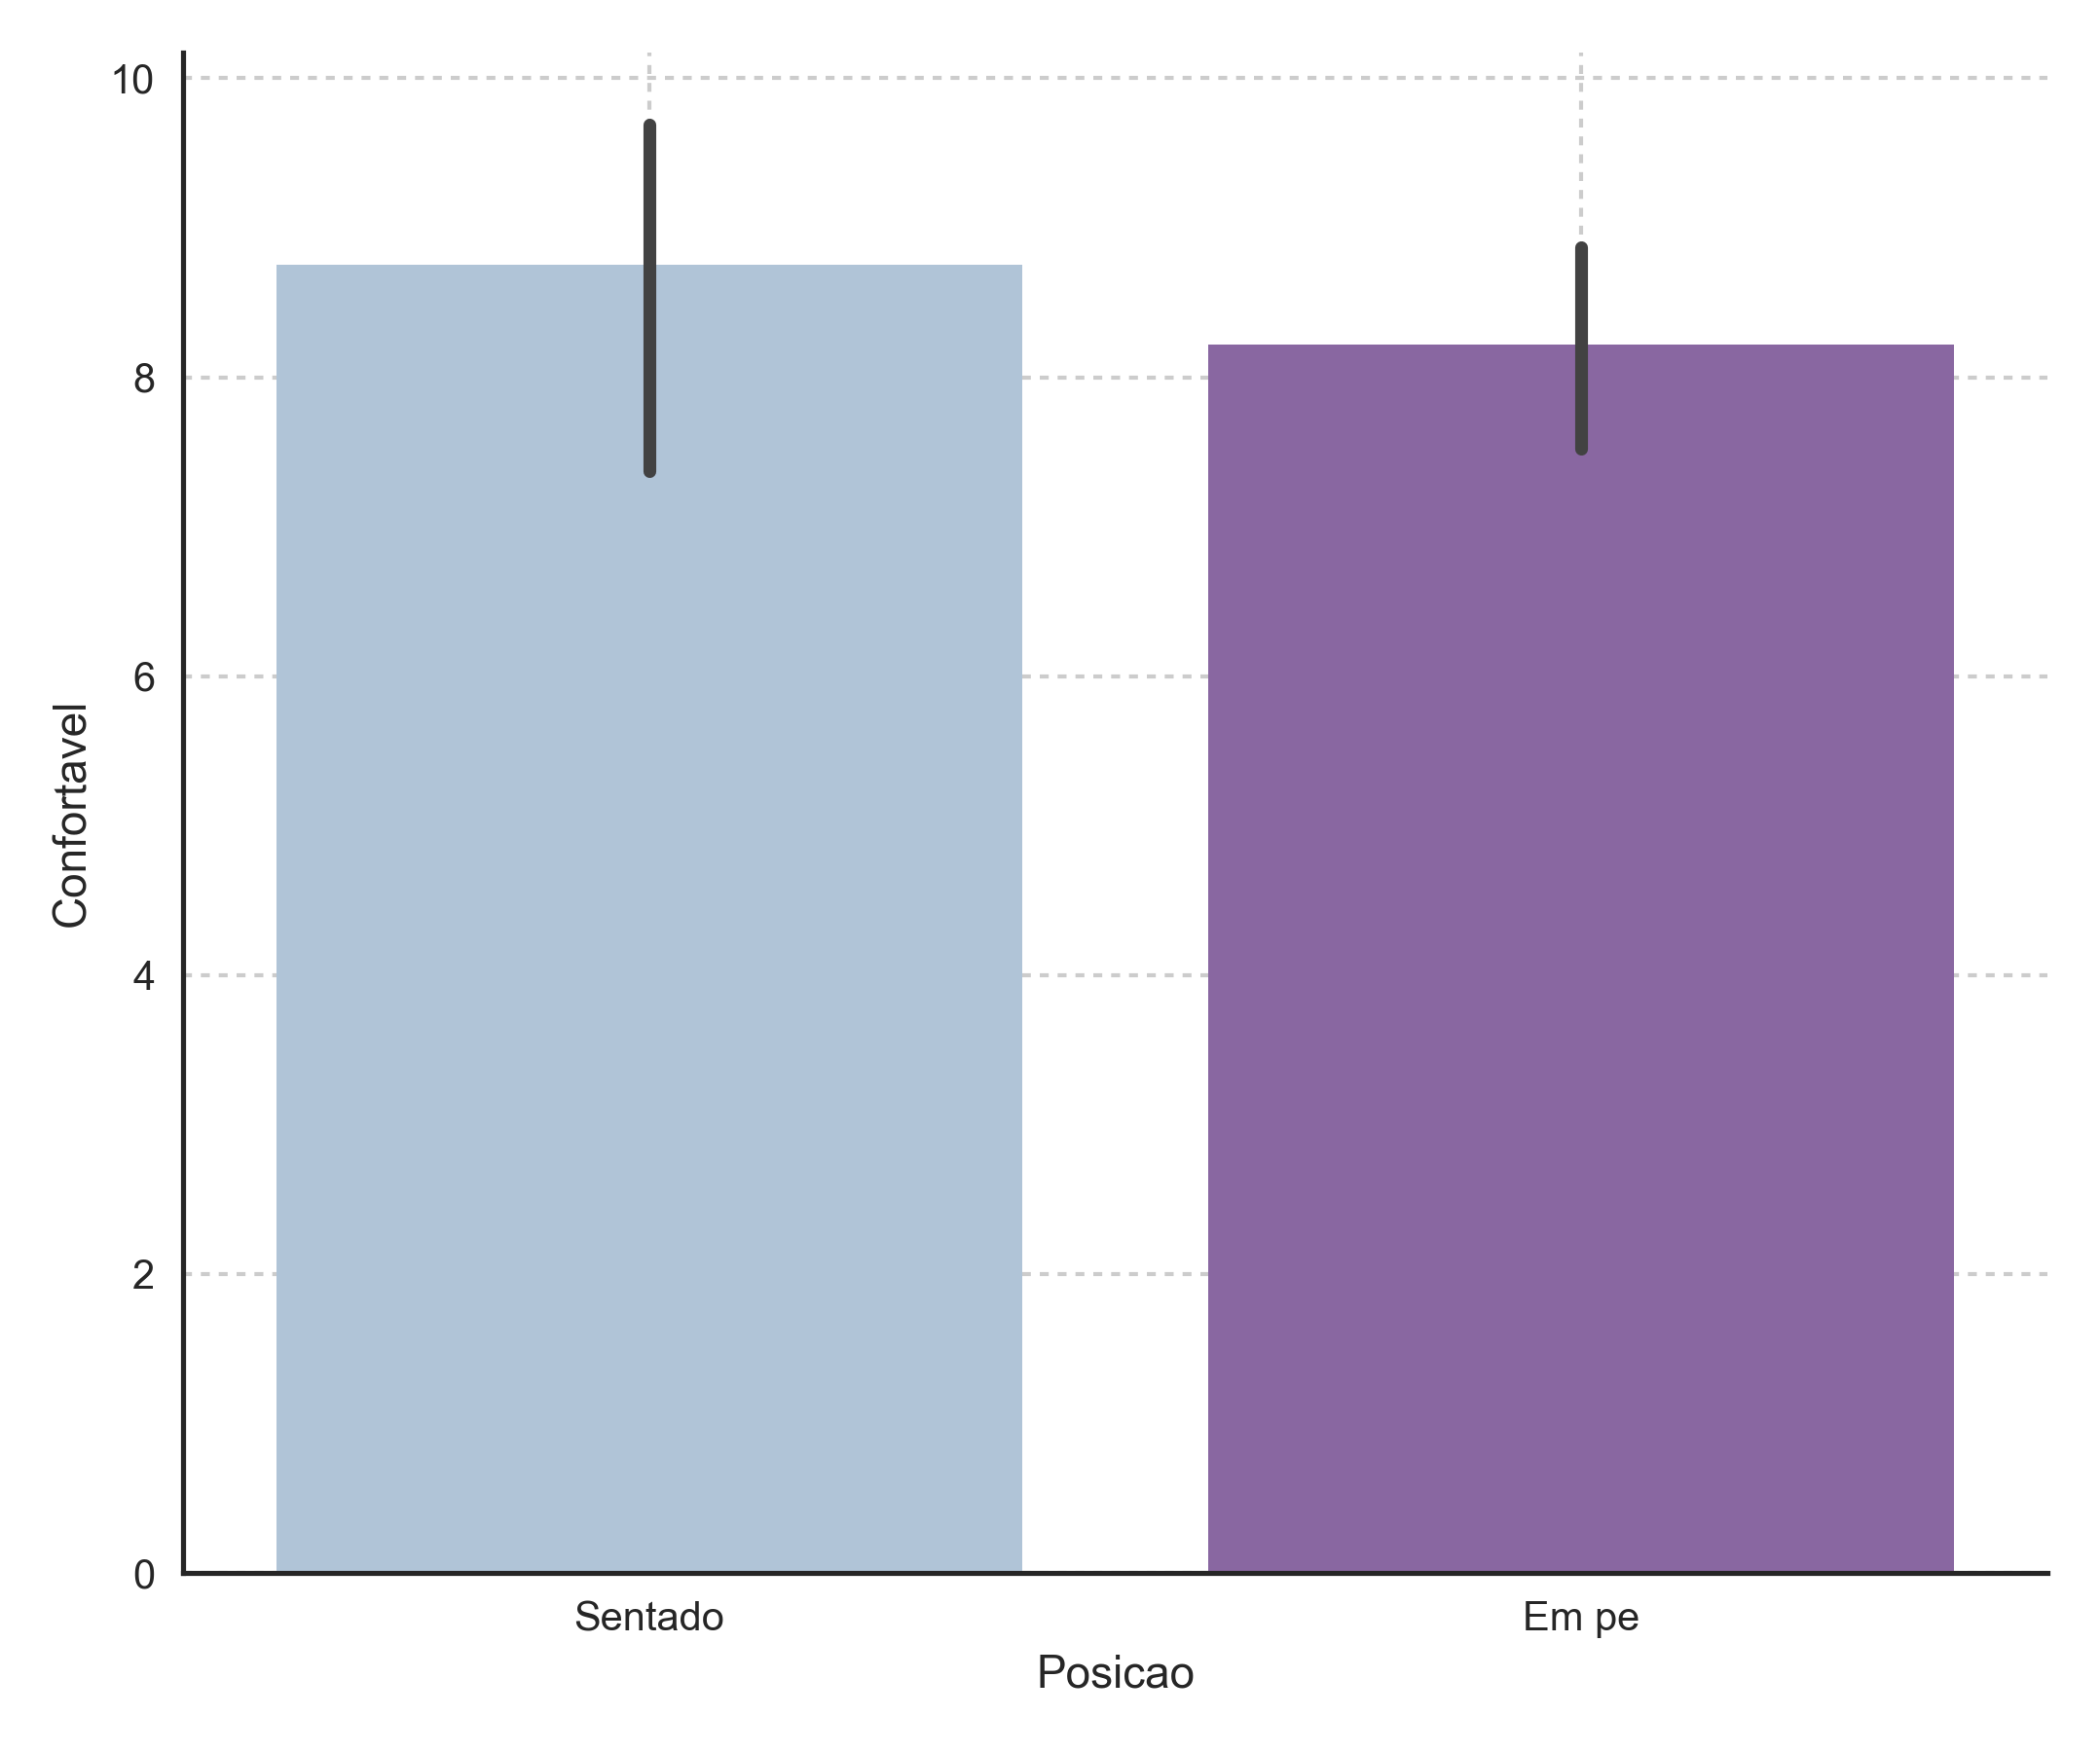
\includegraphics[width=\textwidth]{conforto_posicao.png}
		\smallcaption{Fonte: O autor.}
		\label{fig:confortoposicao}
	\end{minipage}
\end{figure}

É observado na figura~\ref{fig:confortoposicao} o oposto observado na competição da RoboCup@Home. Na competição, as pessoas sentadas sentiram-se com maior desconforto. Nos testes, as pessoas que estavam sentadas durante a interação com o robô sentiram-se mais confortavéis do que as pessoas que estavam em pé. Na média as pessoas em pé apresentaram um grau de conforto igual a 8.2174 e desvio padrão de 1.6407. Já as pessoas sentadas mativeral uma média de 8.75 de grau de conforto, com desvio padrão 2.3848. Esse fenômeno ocorreu, pois o robô tocou no braço e barriga de alguns participantes que estavam em pé quando esticou o manipulador para chamar a atenção deles. O fenômeno do toque é um ponto de atenção que deve ser tratado em uma nova iteração do ciclo de desenvolvimento do projeto, como uma futura evolução no controle do manipulador. Por último, é apresentado na figura~\ref{fig:confortosociavel} o nível de conforto dos participantes, dado a sua declaração de sociável ou não.

\begin{figure}[ht!]
	\centering
	\begin{minipage}{0.65\textwidth}
		\caption{Conforto por declaração de sociável.}
		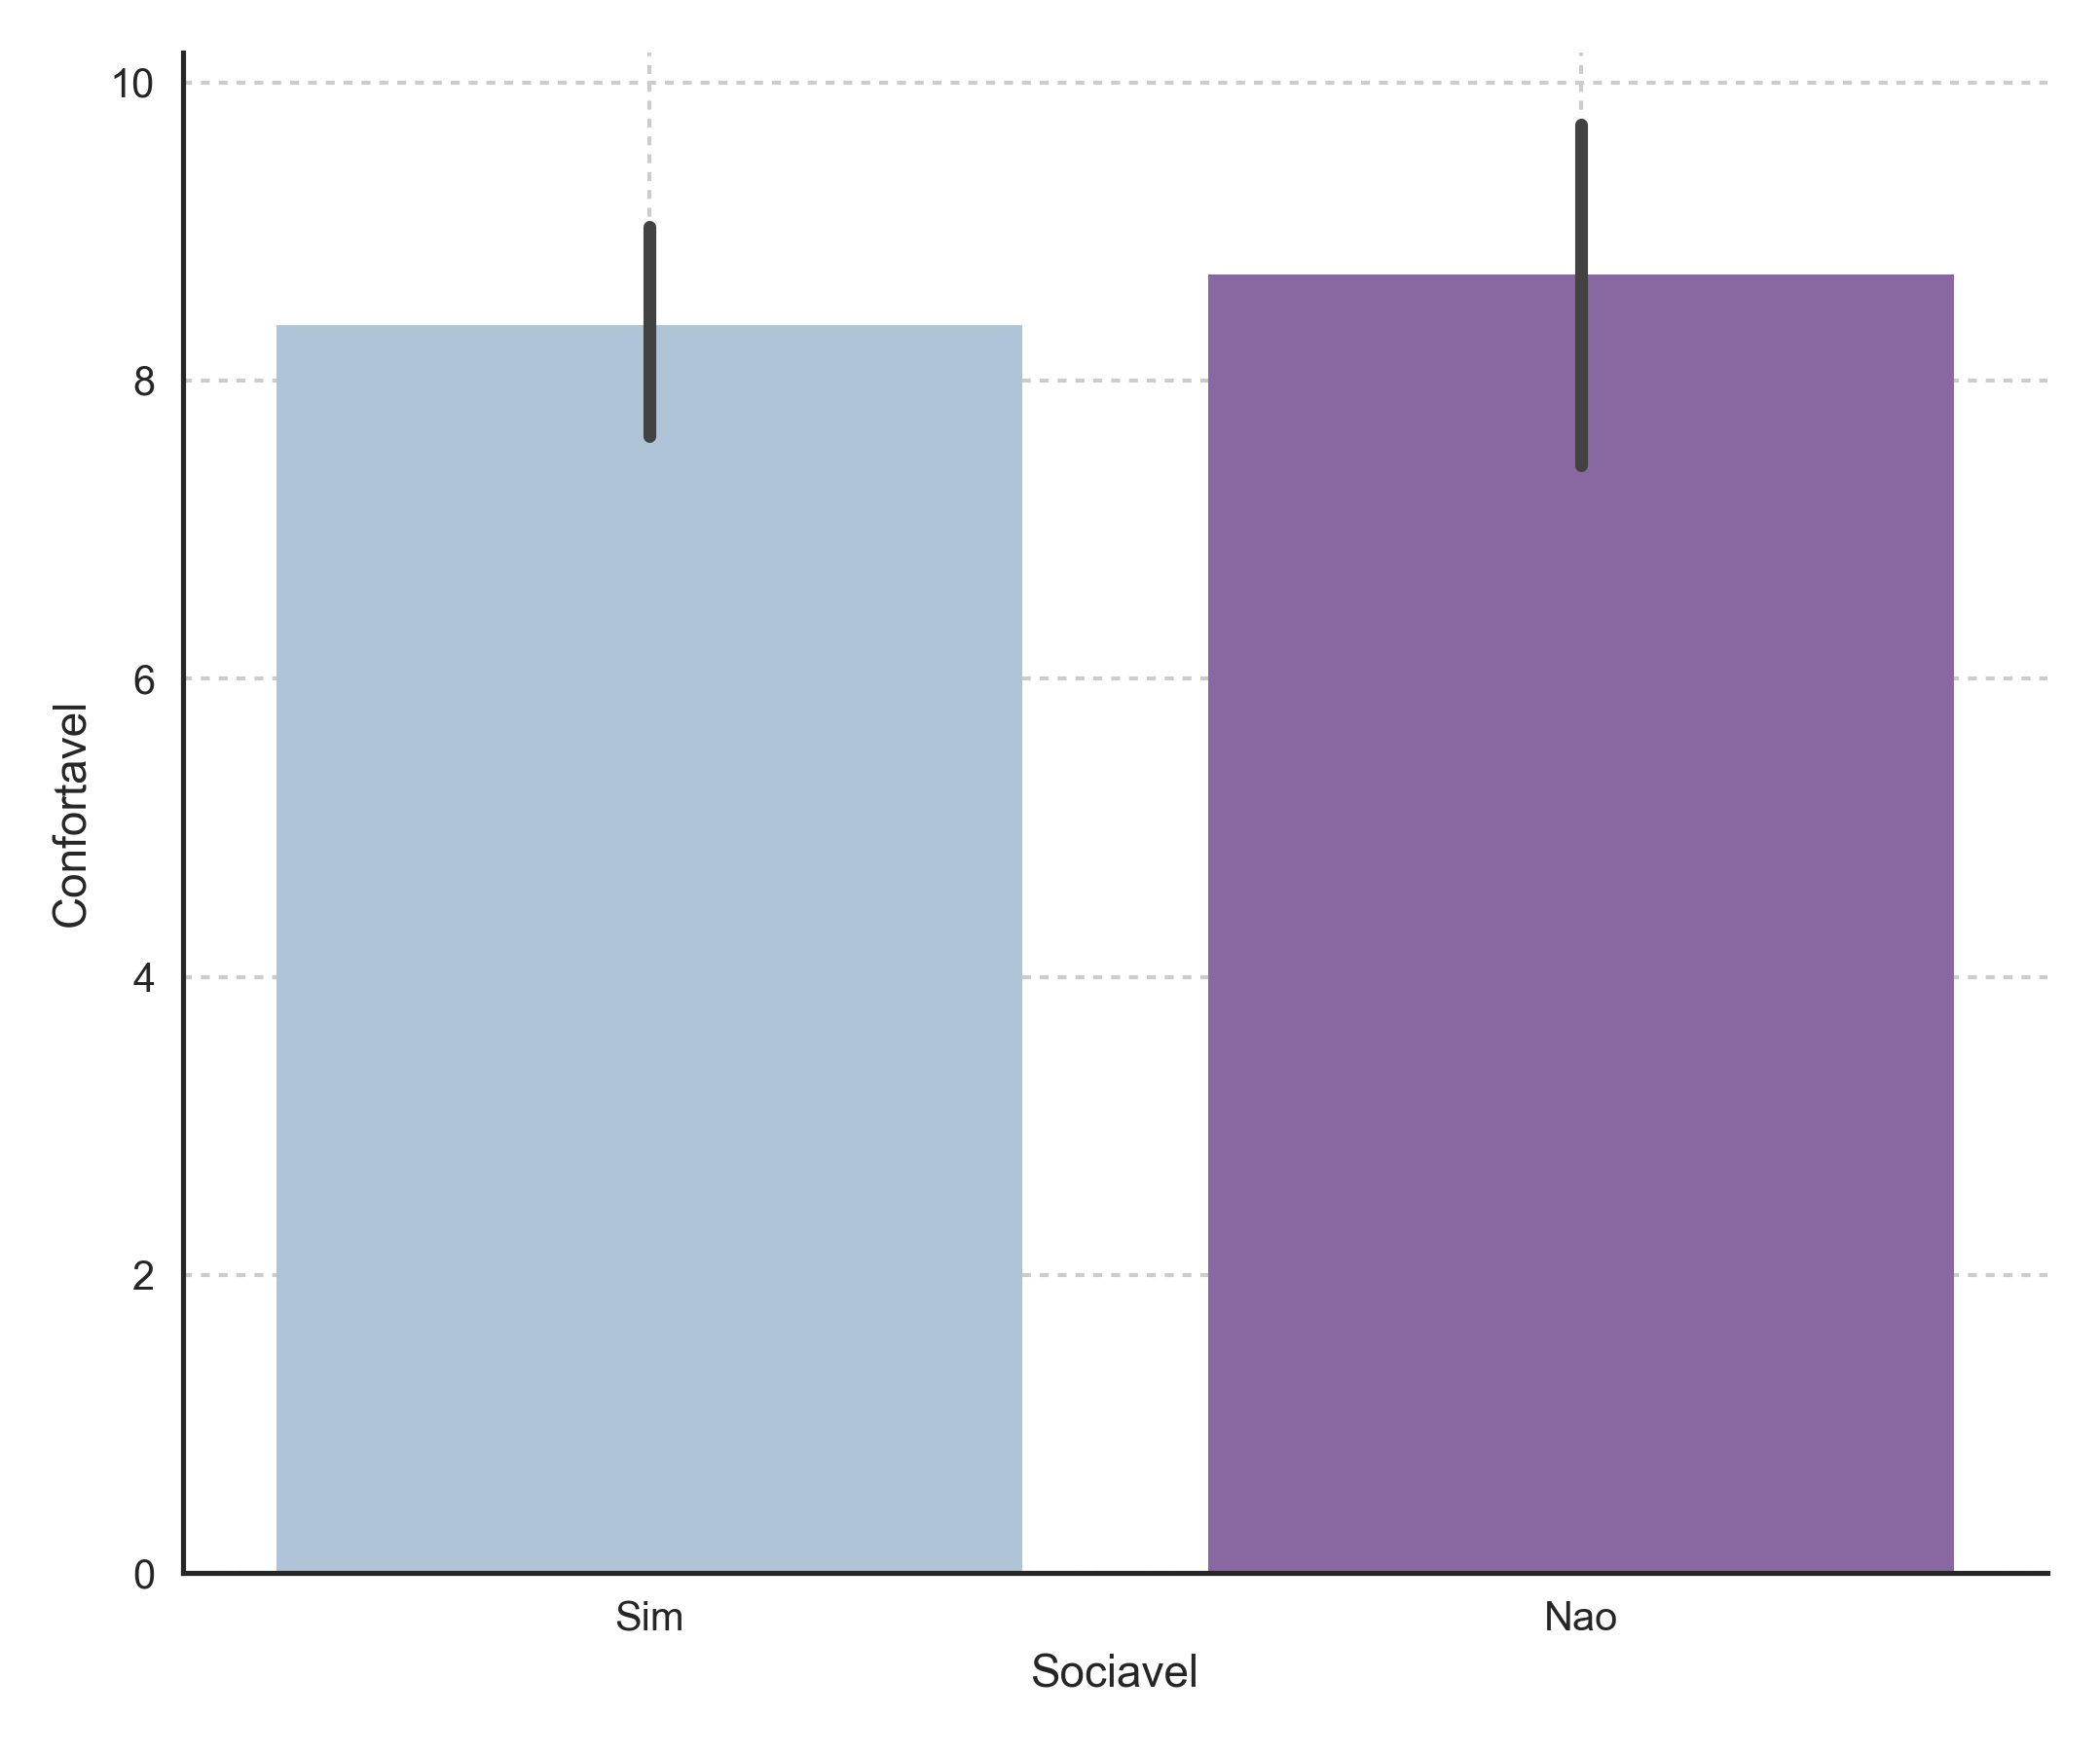
\includegraphics[width=\textwidth]{conforto_sociavel.png}
		\smallcaption{Fonte: O autor.}
		\label{fig:confortosociavel}
	\end{minipage}
\end{figure}

Nessa análise feita através da figura~\ref{fig:confortosociavel}, as pessoas declaradas como não sociáveis, foram as pessoas que mais se sentiram confortáveis durante toda a aproximação do robô. Na média uma pessoa sociável apresentou um grau de conforto de 8.375, com desvio padrão de 2.0729. Já a pessoa não sociável apresentou 8.7143 na média, com desvio padrão de 1.5779. É um ponto interessante, pois se observar, as pessoas sociáveis deveriam estar mais confortável e abertas a novas experiências.

Algumas situações durante o cenário de interação causaram medo, como por exemplo, o manipulador tocado o participante. E na mesma situação, o usuário ficou confortável ao ver a expressão facial amigável do robô, esboçando um sorriso. Assim, a mesma análise para o conforto do usuário, foi realizada para a declaração de medo. Na escala da pergunta sobre medo do robô, o menor valor corresponde a totalmente com medo (valor 0 da escala) e o maior corresponde a totalmente sem medo (valor 10 da escala). A figura~\ref{fig:medogenero} apresenta a relação entre o medo e o gênero do participante.

\begin{figure}[ht!]
	\centering
	\begin{minipage}{0.65\textwidth}
		\caption{Medo por gênero.}
		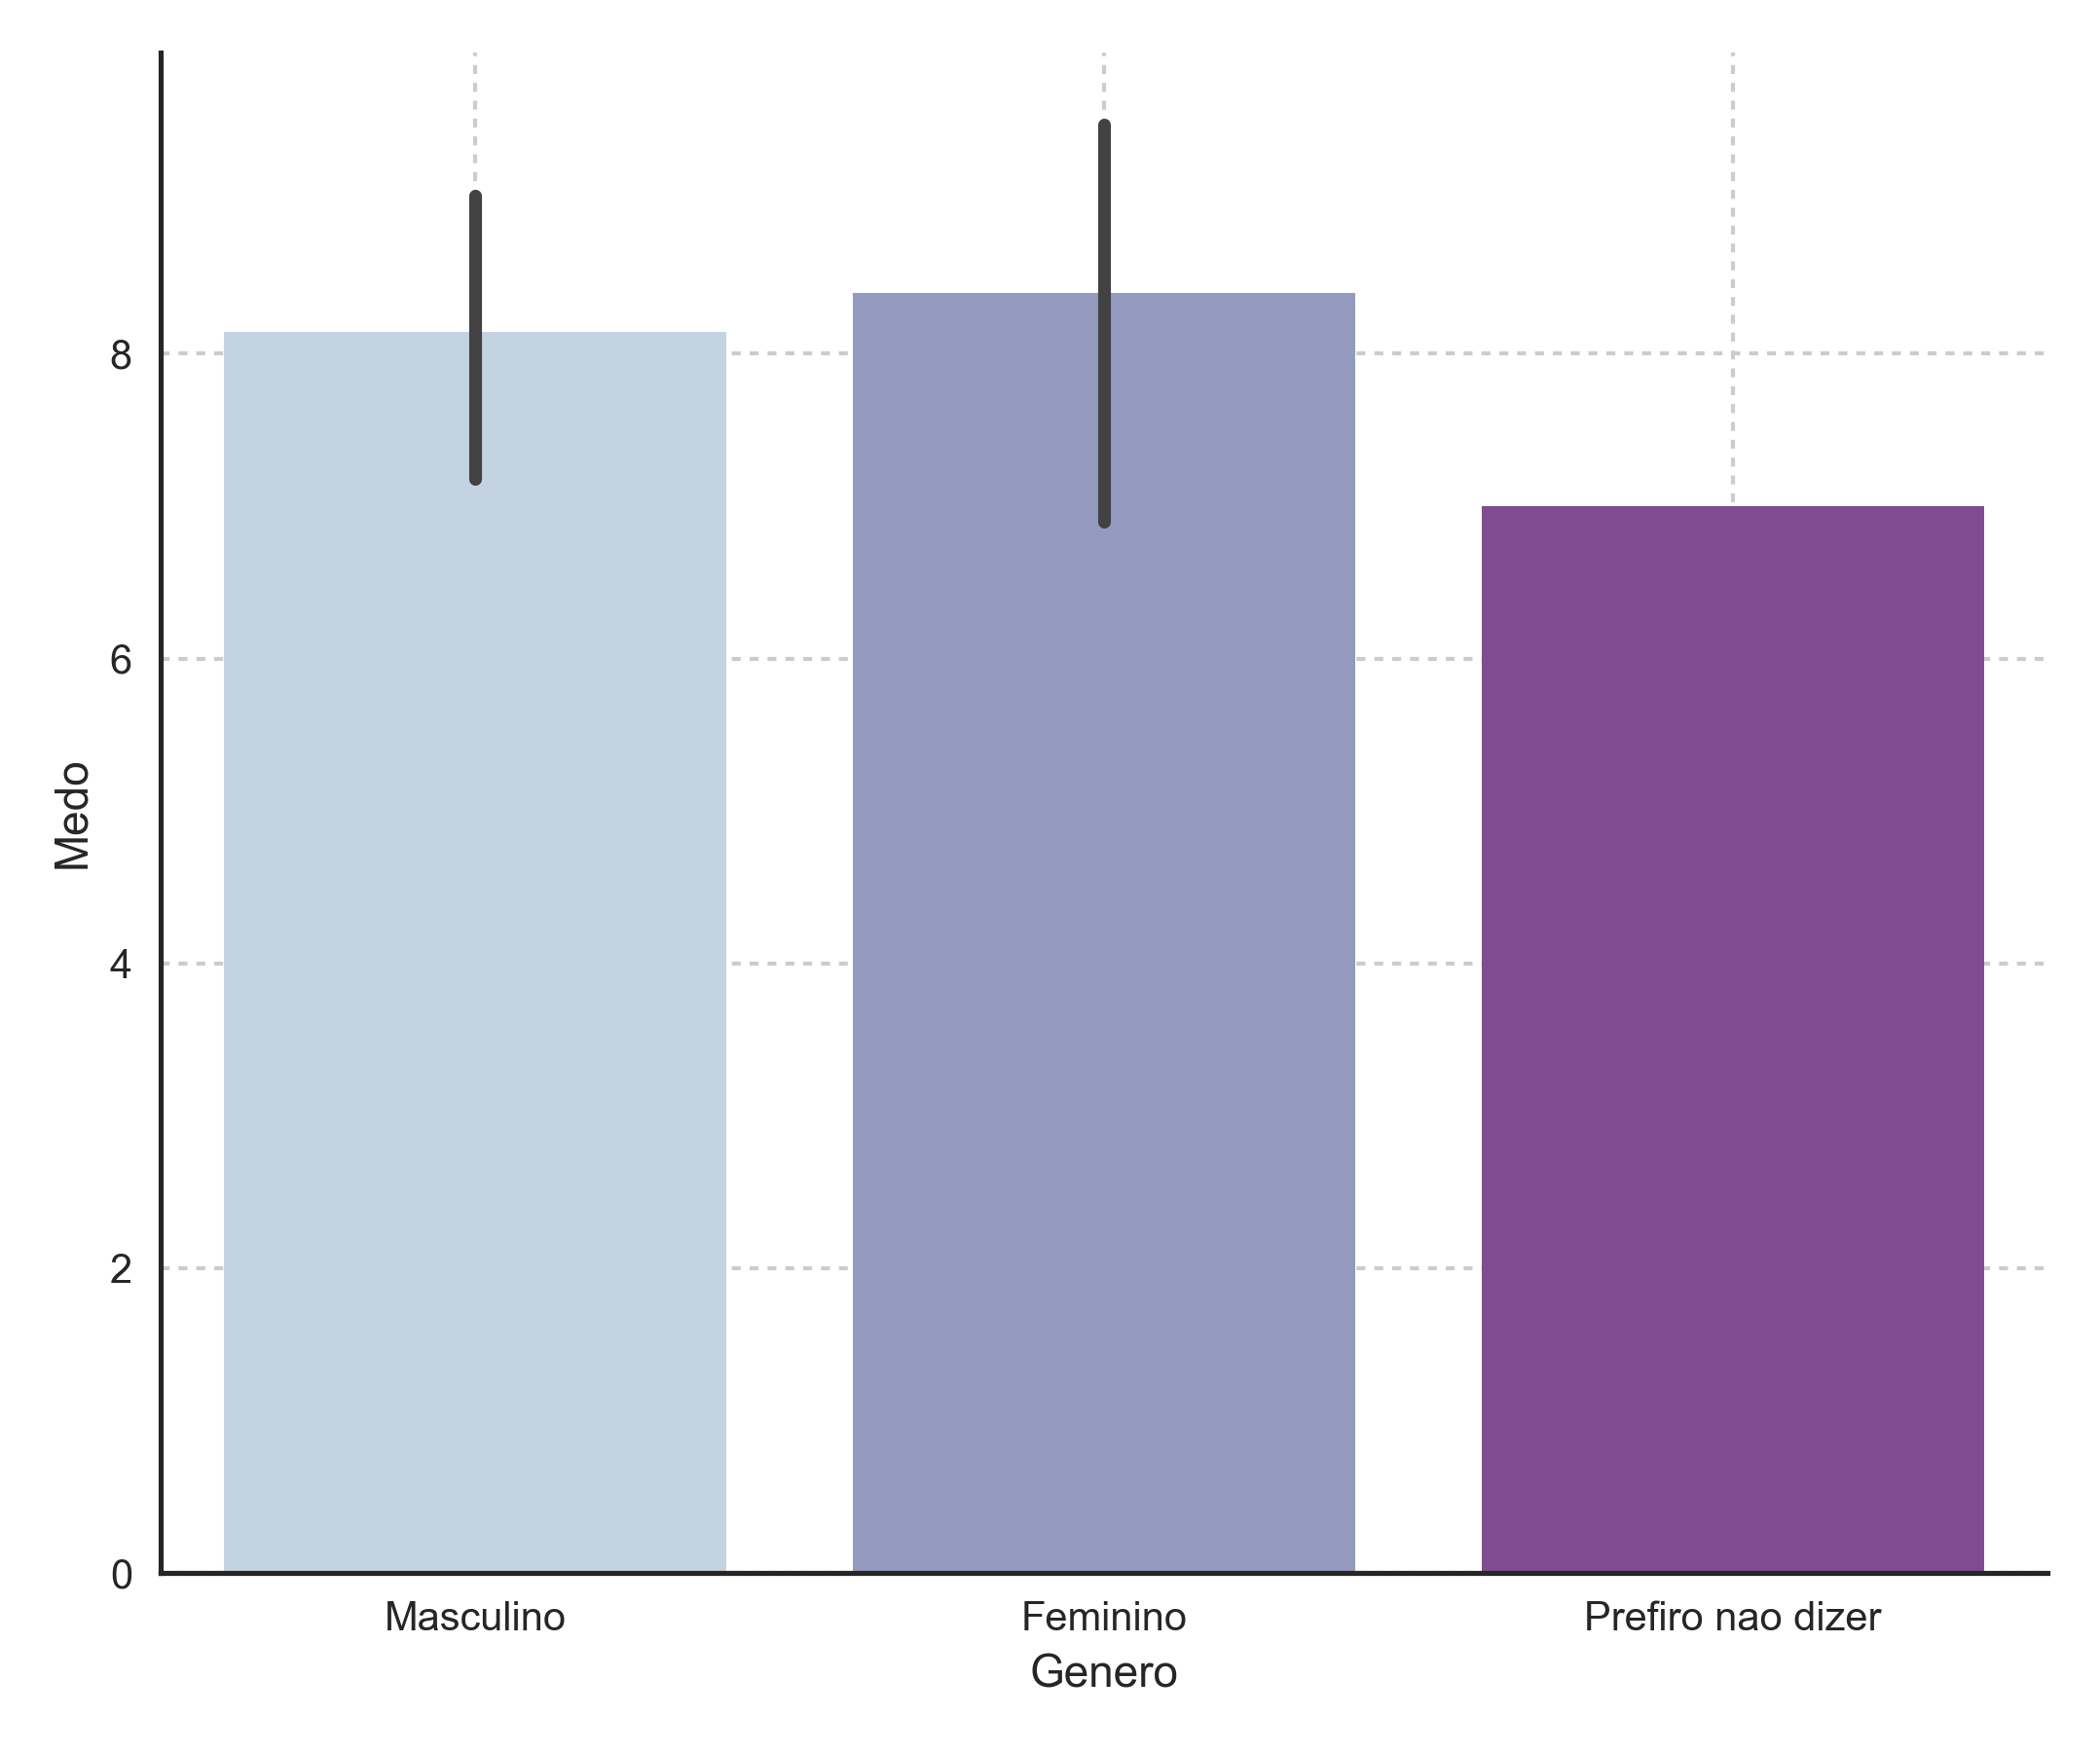
\includegraphics[width=\textwidth]{medo_genero.png}
		\smallcaption{Fonte: O autor.}
		\label{fig:medogenero}
	\end{minipage}
\end{figure}

Para a relação de medo e gênero, o que observa-se na figura~\ref{fig:medogenero} é que o gênero feminino sentiu menos medo. Porém, a diferença não foi tão grande assim. Na média as mulheres tiveram 8.4 graus, com desvio padrão de 2.1071. Enquanto isso, os homens ficaram com a média de 8.1429, desvio padrão de 2.6010. Era esperado este resultado, devido as observações sobre o conforto do usuário, apesar dessa relação nem sempre ser diretamente proporcional. Na sequência é feita a análise com base na relação medo e idade, demonstrada na figura~\ref{fig:medoidade}.

\begin{figure}[ht!]
	\centering
	\begin{minipage}{0.65\textwidth}
		\caption{Medo por idade.}
		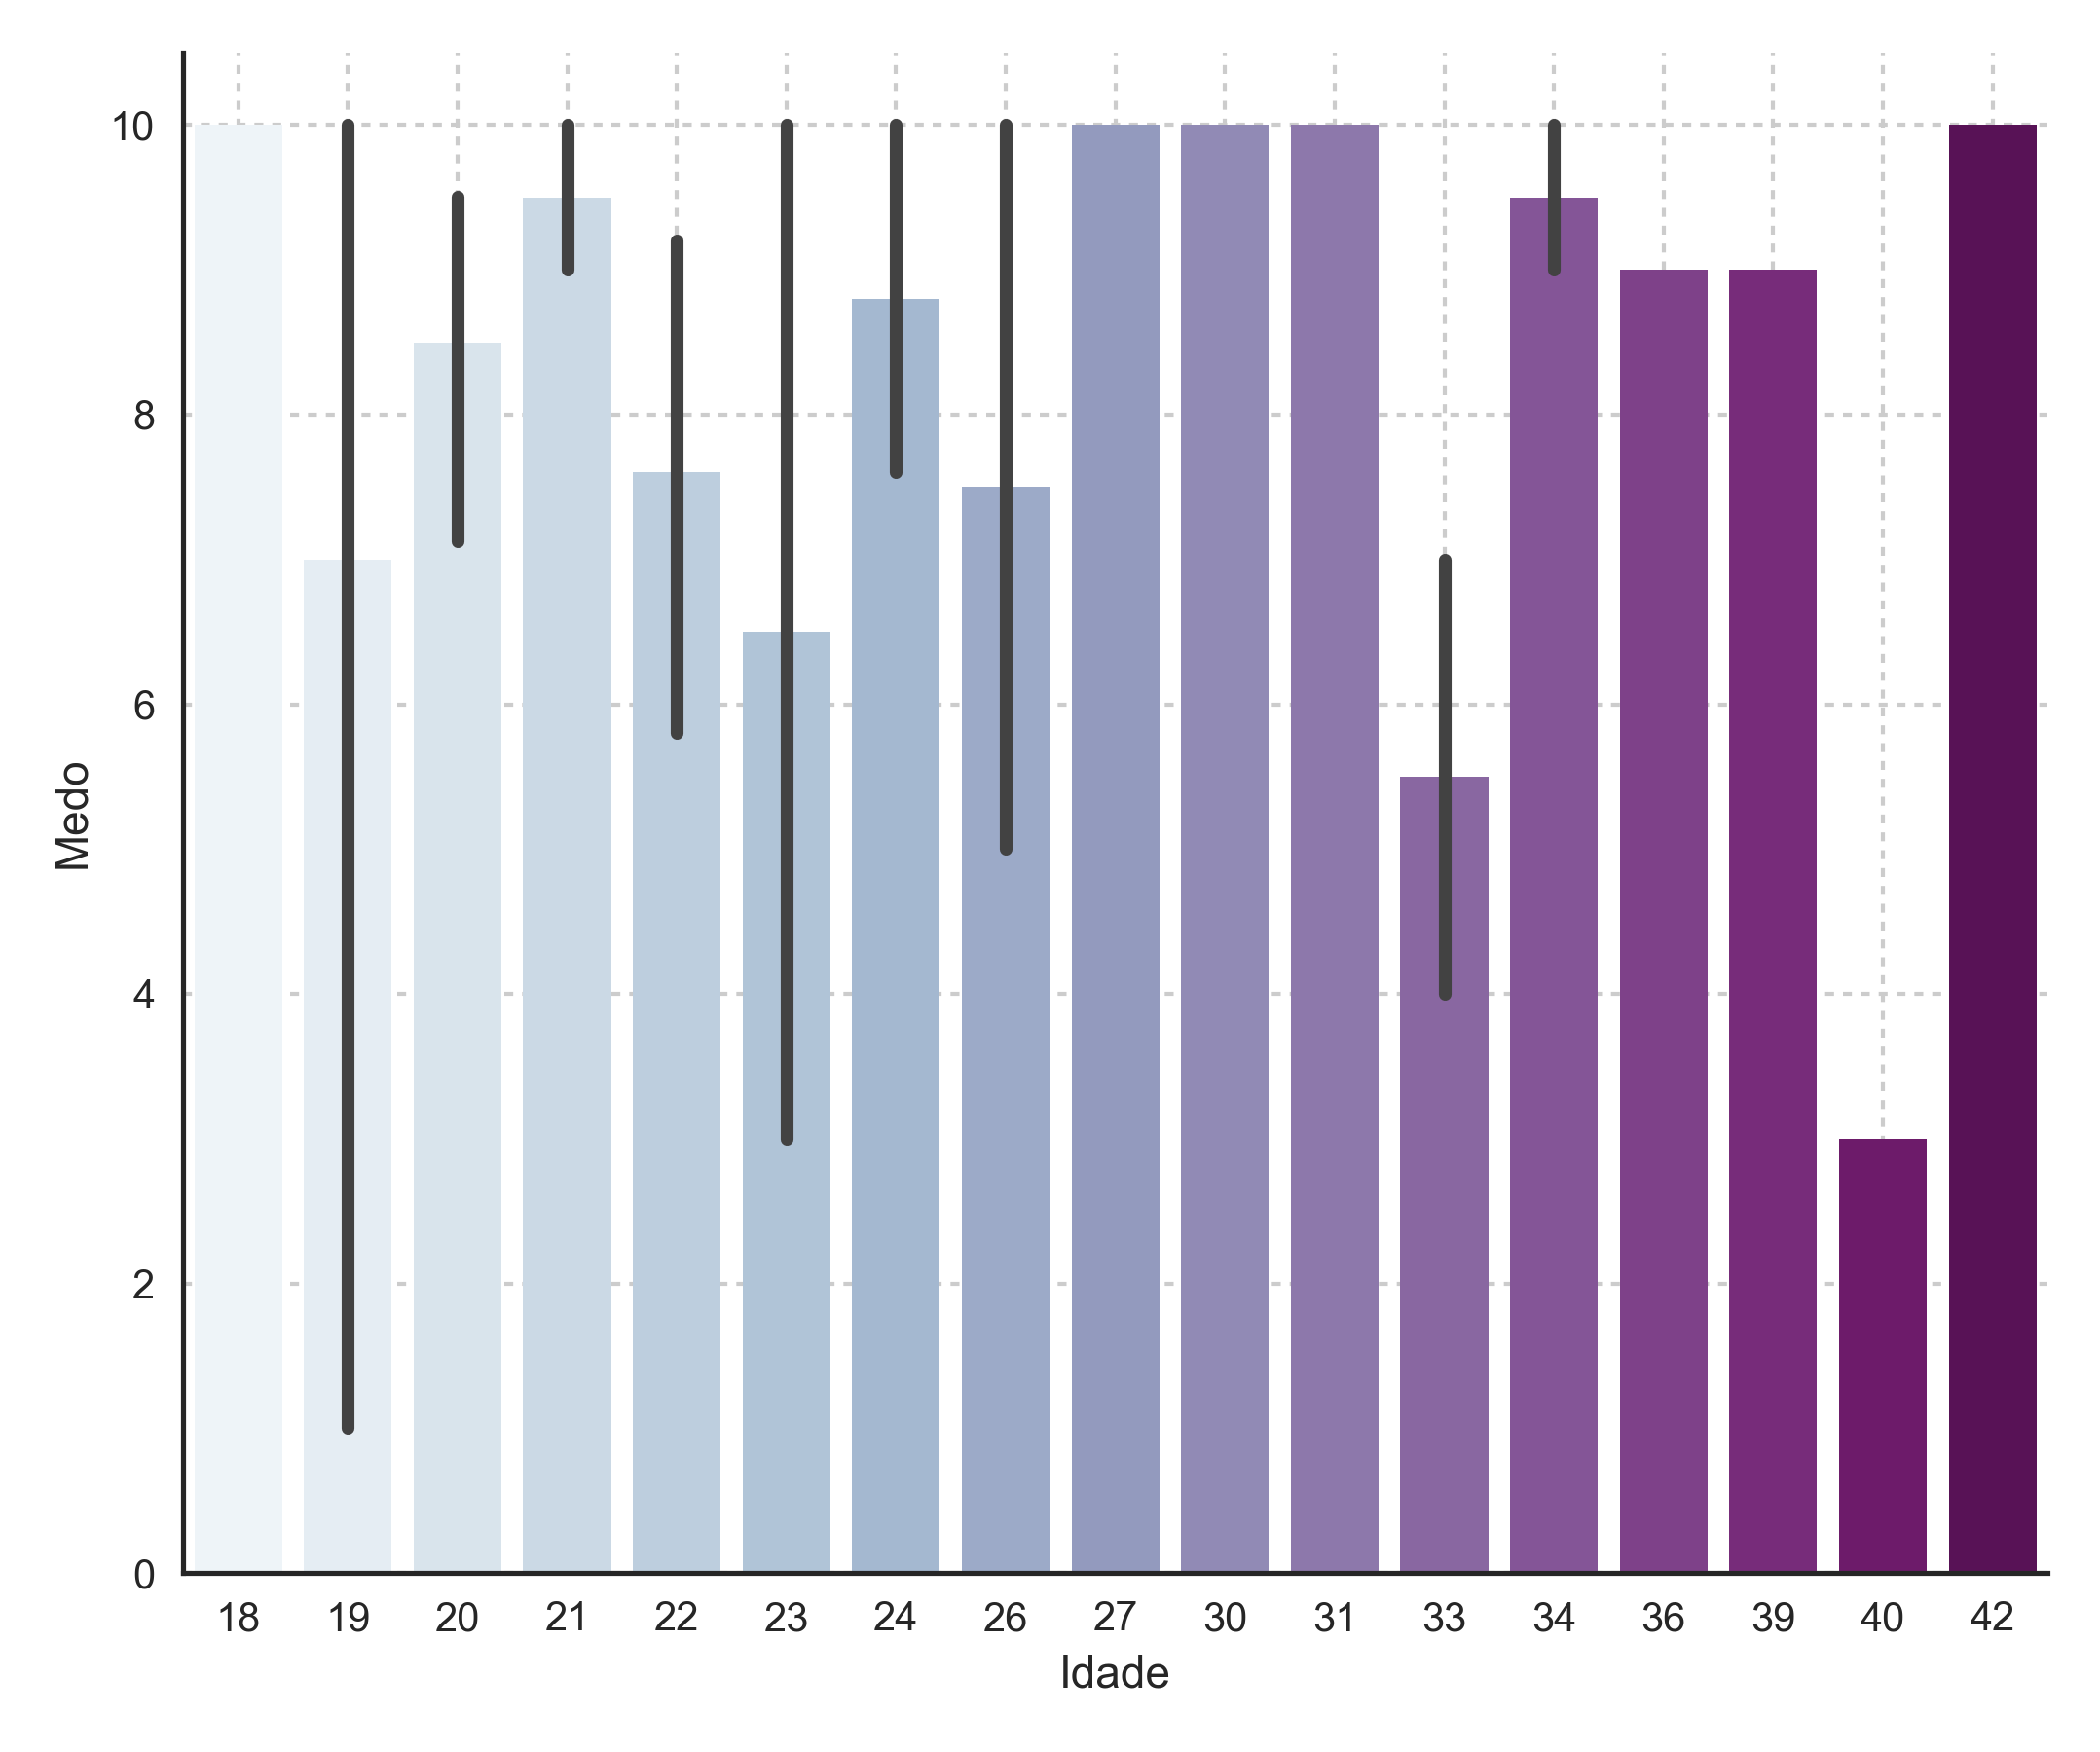
\includegraphics[width=\textwidth]{medo_idade.png}
		\smallcaption{Fonte: O autor.}
		\label{fig:medoidade}
	\end{minipage}
\end{figure}

Um participante na faixa etária de 40 anos, apresentou o maior índice de medo, conforme figura~\ref{fig:medoidade}. Os participantes com 19 anos também apresentam um índice baixo, que indica medo do participante. Isso ocorreu, pois com o comportamento invasivo do robô ao aproximar, a garra deixou o participante assustado. Outro ponto levantado foi que o robô ao se movimentar faz muito barulho, devido ao novo conjunto de rodas omnidirecionais.

A figura~\ref{fig:medoposicao} compara a relação do medo declarado do usuário contra a posição dele durante a navegação do robô.

\begin{figure}[ht!]
	\centering
	\begin{minipage}{0.65\textwidth}
		\caption{Medo por posição de interação.}
		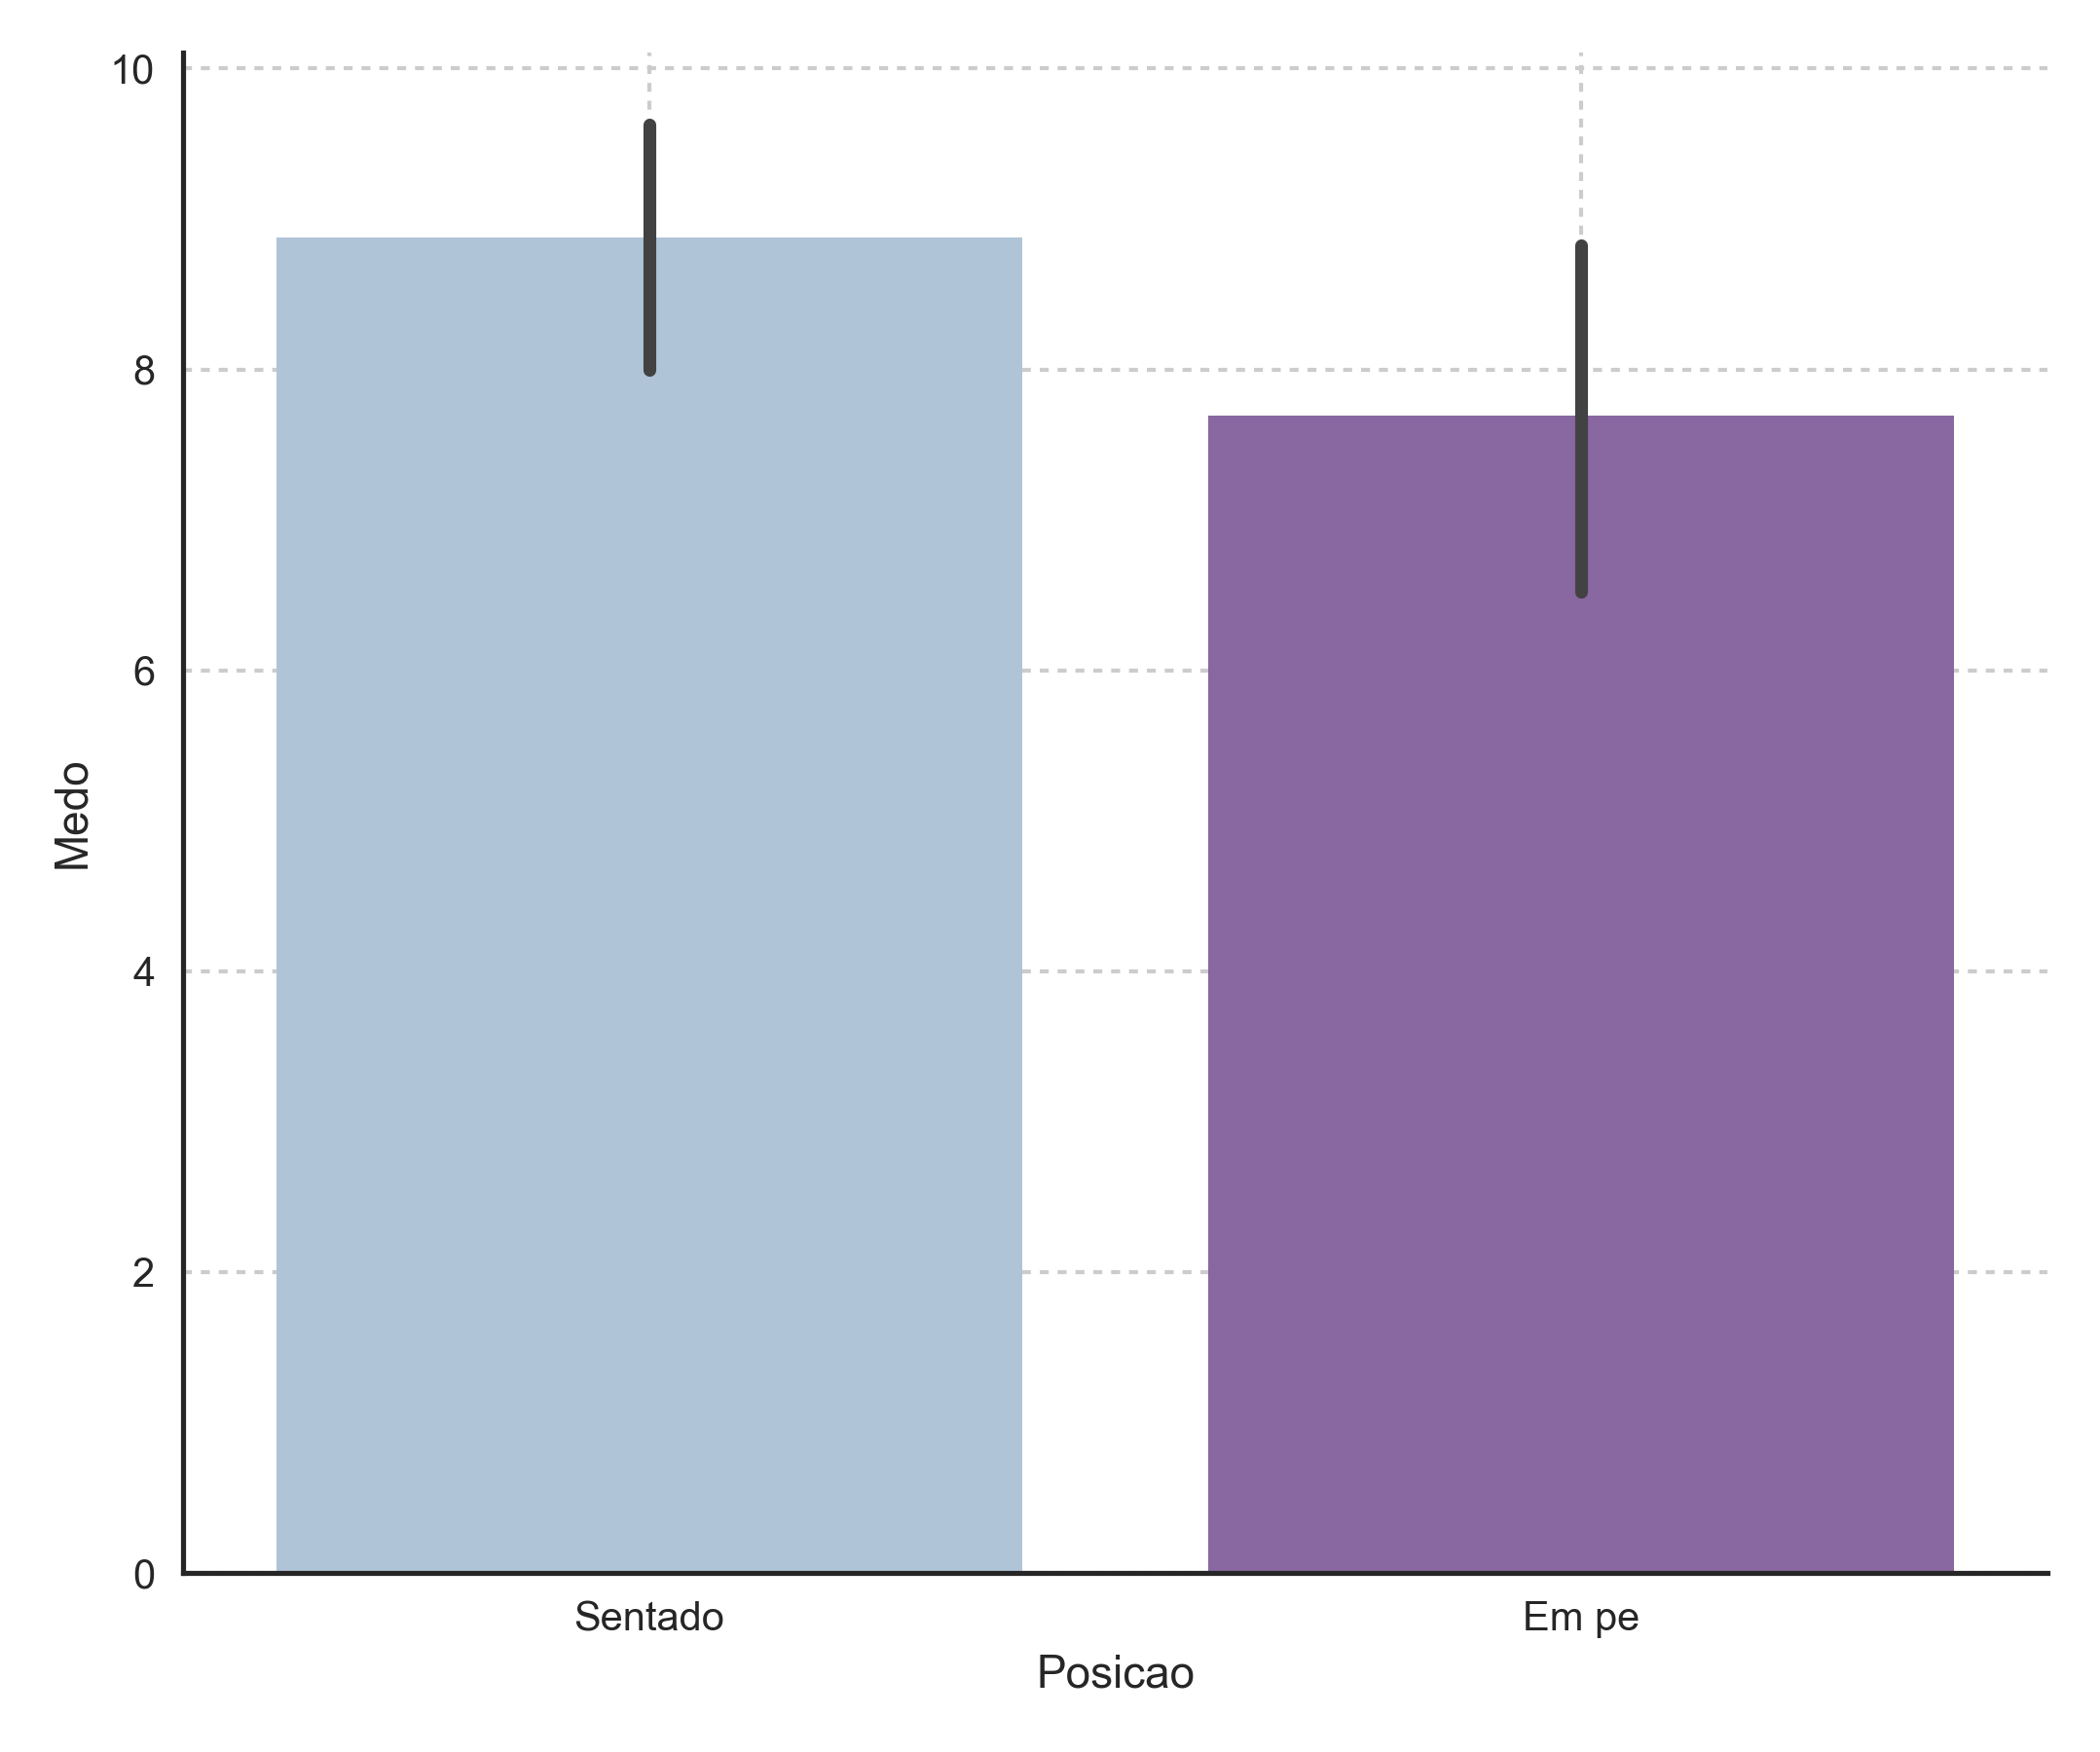
\includegraphics[width=\textwidth]{medo_posicao.png}
		\smallcaption{Fonte: O autor.}
		\label{fig:medoposicao}
	\end{minipage}
\end{figure}

Assim como em relação ao conforto do usuário, os participantes que sentiram mais medo do robô estavam em pé. Os participantes sentados apresentaram uma média de 8.8750, com desvio padrão de 1.6910. Comparando, os participantes em pé tiveram 7.6957 de média e um desvio padrão de 2.7731. O manipulador é um ponto de atenção na interação, principalmente quando está dentro do espaço social da pessoa. Os maiores índices de medo ocorreram por que o robô encostou o manipulador na pessoa, sem nenhum aviso prévio. As pessoas mais sociáveis sentiram menos medo que as menos sociáveis, como apresenta na figura~\ref{fig:medosociavel}. Na média as pessoas sociáveis apresentam 8.4688 contra 6.8571 das pessoas não sociáveis. Os desvios padrão apresentaram os valores 2.0461 e 3.5225, respectivamente.

\begin{figure}[ht!]
	\centering
	\begin{minipage}{0.65\textwidth}
		\caption{Medo por declaração de sociável.}
		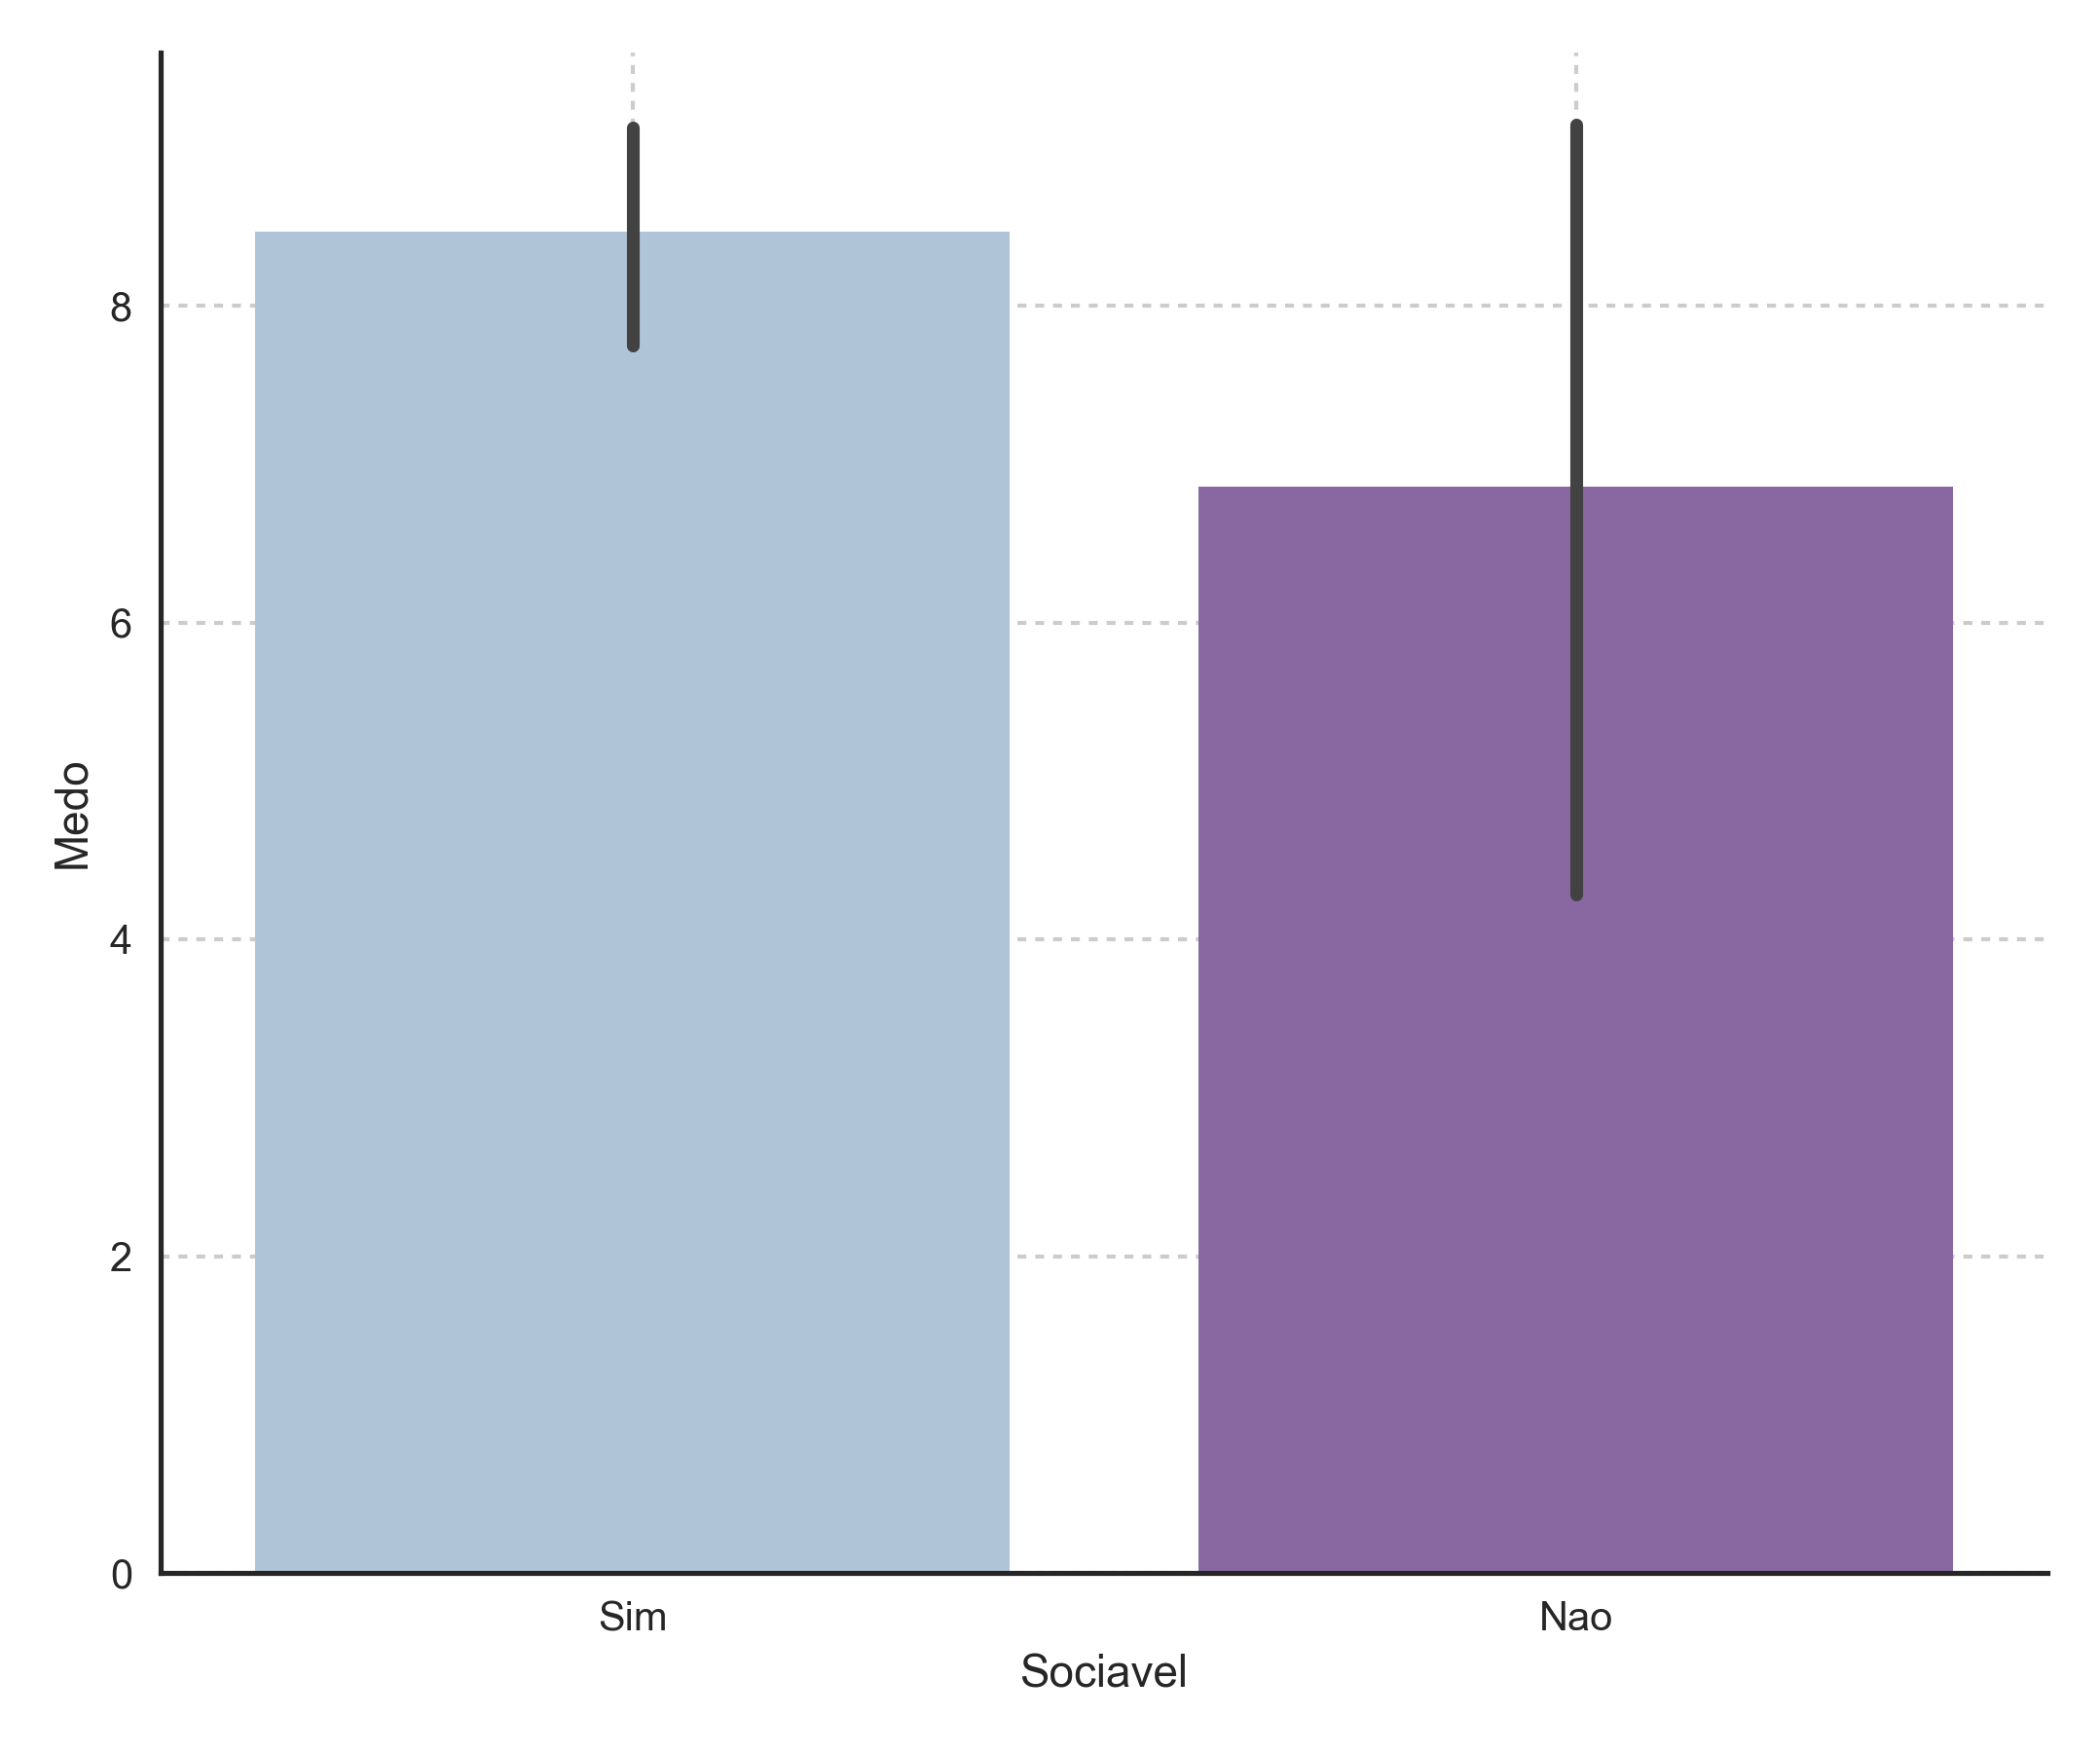
\includegraphics[width=\textwidth]{medo_sociavel.png}
		\smallcaption{Fonte: O autor.}
		\label{fig:medosociavel}
	\end{minipage}
\end{figure}

Após as análises gerais sobre as informações coletadas, é realizado o processo para obter os grupos de perfis de usuários, conforme seção~\ref{sec:criacaopersonas}. Para obter os grupos de perfis, utilizou-se o algoritmo de agrupamento por similaridade QG-SIM. Foram testados três valores Q, que determinam a similaridade mínima do grupo, para determinar os grupos. Os valores utilizados foram 0.6, 0.7 e 0.8. O valor 0.6 resultou em 3 grupos, porém um dos grupos manteve 90\% dos perfis e ou outros 10\% foram distribuídos entre os dois grupos restantes. O valor $Q = 0.6$ apresentou resultado muito generalizado e que não condiz com os perfis que realizaram os testes.

Quando aplicado o valor de 0.8 de similaridade para o algoritmo, 7 grupos foram encontrados. Nessa situação, os grupos ficaram bem específicos, sendo que 4 dos 7 grupos eram compostos por apenas 1 pessoa. Dessa maneira, é possível comprovar que o resultado gerado é muito especializado. Elevar o grau de similaridade nesse ponto, provavelmente serão encontrados mais grupos com apenas uma pessoa. Esse não é o objetivo da técnica de Personas. Então este resultado também foi desconsiderado.

O valor intermediário, 0.7, foi escolhido. Ele resultou em 5 grupos. Um grupo com 21 perfis, que resultou na Persona Joaquim (vide tabela~\ref{tab:joaquim}). Um grupo com 7 pessoas para Persona Maria Eduarda (vide tabela~\ref{tab:mariaeduarda}). Outro grupo com 9 pessoas deu origem a Persona Alfredo (vide tabela~\ref{tab:alfredo}). As outras duas Personas foram criadas com base em dois grupos de 1 pessoa. Apesar de serem formados por apenas 1 pessoa, algumas características foram totalmente descriminante. A Persona Manuel (vide tabela~\ref{tab:manuel}), por exemplo, não tem acesso, nem conta em redes sociais. E a Persona Danielo (vide tabela~\ref{tab:danielo}) aplicou a nota positiva máxima em todas as situações de interação. Esses fatores foram decisivos para que esses perfis permanecessem isolados em um grupo cada um.

Cada perfil dentro dos grupos mantém uma consistência etnográfica e também sobre a percepção em relação aos comportamentos e ações do robô. As percepções de cada perfil, estão sintetizadas e são apresentadas em grupos de informações similares. Essas informações auxiliaram na descrição de cada Persona. A tabela~\ref{tab:expectativacasa} apresenta um compilado das informações referentes a expectativa de ter um robô em casa, na percepção de cada usuário.

\begin{table}[!ht]
	\caption{Expectativa do robô em casa dos perfis por Persona.}
	\label{tab:expectativacasa}
	\centering
	\begin{tabular}{c | c | c }
        \hline
        \multicolumn{3}{c}{Expectativa do robô em casa?} \\ \hline
        Persona & Observação & Quantidade \\ \hline
        \multirow{7}{*}{Joaquim} & Limpar a casa & 7 \\
        \hhline{~--}
        & Buscar objetos & 1 \\
        \hhline{~--}
        & Cuidar da segurança & 1 \\
        \hhline{~--}
        & Obediência & 4 \\
        \hhline{~--}
        & Afetividade & 4 \\
        \hhline{~--}
        & Naturalidade & 3 \\
        \hhline{~--}
        & Respeito & 3 \\
        \hline
        \multirow{3}{*}{Maria Eduarda} & Realizar tarefas domésticas & 5 \\
        \hhline{~--}
        & Dirigir o carro & 1 \\
        \hhline{~--}
        & Amigável & 1 \\
        \hline
        \multirow{4}{*}{Alfredo} & Realizar tarefas domésticas & 5 \\
        \hhline{~--}
        & Comandos de voz & 2 \\
        \hhline{~--}
        & Obediência & 2 \\
        \hline
        Danielo & Realizar tarefas domésticas & 1 \\
        \hline
        Manuel & Atender necessidades & 1 \\
        \hline
    \end{tabular}
    \smallcaption{Fonte: O autor.}
\end{table}

A pergunta da expectativa do robô em casa foi realizada antes da interação com o robô. Com base nas respostas pode-se perceber que as pessoas, no geral, enxergam os robôs como ferramentas. Essa percepção muda após a interação e a demonstração das habilidades dos robôs. Em alguns casos, a mudança de opinião é nítida, onde comentários como ``ele faz tudo isso sozinho'' são mencionados durante o teste. Ou quando o usuário diz que imagina robôs apenas na linha de produção de fábricas e montadores. Outra questão discutida antes da interação com o robô é a expectativa sobre o papel dele, em relação ao ambiente de trabalho. As respostas compiladas são apresentadas na tabela~\ref{tab:expectativatrabalho}.

\begin{table}[!ht]
	\caption{Expectativa do robô no ambiente de trabalho dos perfis por Persona.}
	\label{tab:expectativatrabalho}
	\centering
	\begin{tabular}{c | c | c }
        \hline
        \multicolumn{3}{c}{Expectativa do robô no ambiente de trabalho?} \\
        \hline
        Persona & Observação & Quantidade \\
        \hline
        \multirow{10}{*}{Joaquim} & Obediência & 4 \\
        \hhline{~--}
        & Realizar tarefas & 7 \\
        \hhline{~--}
        & Indiferente sobre o robô no trabalho & 1 \\
        \hhline{~--}
        & Eficiência nas atividades & 2 \\
        \hhline{~--}
        & Comunicação & 1 \\
        \hhline{~--}
        & Antecipar tarefas & 1 \\
        \hhline{~--}
        & Gerenciador de \emph{TODO List} & 1 \\
        \hhline{~--}
        & Otimizar processos & 1 \\
        \hhline{~--}
        & Seja sociável & 1 \\
        \hhline{~--}
        & Agir com naturalidade & 2 \\
        \hline
        \multirow{3}{*}{Maria Eduarda} & Realizar tarefas & 4 \\
        \hhline{~--}
        & Eficácia & 1 \\
        \hhline{~--}
        & Amigável & 1 \\
        \hline
        \multirow{3}{*}{Alfredo} & Realizar tarefas & 6 \\
        \hhline{~--}
        & Rápido & 1 \\
        \hhline{~--}
        & Obediência & 1 \\
        \hline
        Danielo & Executar tarefas repetitivas & 1 \\
        \hline
        Manuel & Atender necessidades & 1 \\
        \hline
    \end{tabular}
    \smallcaption{Fonte: O autor.}
\end{table}

Apesar da expectativa no trabalho ser a realização de tarefas, em linhas gerais, alguns outros pontos foram levantados. Comunicação, naturalidade, ser amigável e sociável, além de outros adjetivos voltados para convívio social em ambientes corporativos. Essa percepção pode mostrar tendências para aceitar trabalho em equipe com robôs autonômos de maneira natural. As tabelas a seguir são de informações que foram coletadas após o experimento de interação social com o robô. A tabela~\ref{tab:agradou} apresenta as percepções sobre o robô, que os participantes mais e menos gostaram.

\begin{table}[!ht]
	\caption{O que os perfis mais gostaram e menos gostaram separados por Persona.}
	\label{tab:agradou}
	\centering
	\begin{tabular}{c | c | c | c | c}
        \hline
        \multirow{2}{*}{Persona} & \multicolumn{2}{c}{(+) Gostou} & \multicolumn{2}{c}{(-) Gostou} \\
        \hhline{~----}
		& Observação & Quantidade & Observação & Quantidade \\
		\hline
        \multirow{9}{*}{Joaquim} & Navegação & 4 & Desajeitado & 7 \\
        \hhline{~----}
		& Face & 12 & Tempo de localização & 2 \\
        & & & no ambiente &  \\
        \hhline{~----}
        & Voz & 6 & Barulho das rodas & 4 \\
        \hhline{~----}
        & Manipulador & 1 & Feedback baixo & 1 \\
        \hhline{~----}
        & & & Manipulador & 1 \\
        \hhline{~----}
		& & & Rodas & 1 \\
        \hhline{~----}
		& & & Fala autoritária & 1 \\
        \hhline{~----}
		& & & Tempo de resposta & 1 \\
        \hline
        \multirow{4}{*}{Maria Eduarda} & Navegação & 4 & Estrutura & 2 \\
        \hhline{~----}
        & Interação & 1 & Manipulador & 2 \\
        \hhline{~----}
        & Face & 3 & Barulho & 1 \\
		\hhline{~----}
        & & & Tempo de Resposta & 1 \\
        \hline
        \multirow{6}{*}{Alfredo} & Face & 2 & Tempo de Resposta & 2 \\
        \hhline{~----}
        & Voz & 2 & Desajeitada & 1 \\
        \hhline{~----}
        & Navegação & 1 & Manipulador & 3 \\
		\hhline{~----}
        & Feedback & 1 & Barulho & 1 \\
		\hhline{~----}
        & Toque & 1 & Perda da localização & 1 \\
		\hhline{~----}
        & Interação & 2 & & \\
        \hline
        Danielo & Interação & 1 & Barulho & 1 \\
        \hline
        Manuel & Face e voz & 1 & Manipulador & 1 \\
        \hline
    \end{tabular}
    \smallcaption{Fonte: O autor.}
\end{table}

Através da tabela~\ref{tab:agradou} é possível observar quais pontos do robô, e até como as variáveis de percepção do usuário que foram criadas com base nas heurísticas de interação (vide seção~\ref{sec:heuristicas}), se relacionam com cada perfil. A visibilidade do estado do robô é um dos pontos mais observados entre os usuários. A relação de \emph{feedback} do robô, algumas das Personas apontaram como positivo e outras como negativo, pois não foi realizado de maneira adequada. Outro ponto levantado, é a questão do barulho feito pela base do robô, onde 4 das 5 Personas observaram isso como um problema. Além dos pontos positivos e negativos do robô durante a interação, as informações sobre quais pontos geraram desconforto ou medo são importantes. As informações sobre desconforto são apresentadas na tabela~\ref{tab:desconforto}.

\begin{table}[!ht]
	\caption{Desconforto dos perfis na interação, separados por Persona.}
	\label{tab:desconforto}
	\centering
	\begin{tabular}{c | c | c }
        \hline
        Persona & Observação & Quantidade \\
        \hline
        \multirow{3}{*}{Joaquim} & Quase batida no ambiente & 1 \\
        \hhline{~--}
        & Primeira aproximação & 4 \\
        \hhline{~--}
        & Balanço da estrutura & 1 \\
        \hline
        \multirow{2}{*}{Maria Eduarda} & Manipulador & 1 \\
        \hhline{~--}
        & Aproximação & 1 \\
        \hline
        \multirow{3}{*}{Alfredo} & Falta de feedback & 2 \\
        \hhline{~--}
        & Toque & 1 \\
        \hhline{~--}
        & Aproximação & 2 \\
        \hline
        Danielo & -- & -- \\
        \hline
        Manuel & Manipulador & 1 \\
        \hline
    \end{tabular}
    \smallcaption{Fonte: O autor.}
\end{table}

Na tabela~\ref{tab:desconforto} pode-se evidenciar que a aproximação do robô, principalmente ao entrar no espaço pessoal e intímo da pessoa, gera um nível de desconforto significante. Quando ocorre o toque no participante esse desconforto pode levar a um nível de medo para alguns participantes na interação. O controle da aproximação e da invasão das zonas sociais definidas através da teoria de proximidade (capítulo~\ref{cap:proxemics}) é importante para melhorar a experiência do usuário e conseguir manter uma interação de longo prazo em outros cenários. As questões relacionadas a proximidade do robô, não condizem apenas com a ação de aproximição. A proximidade é um fator importante que pode influenciar em gestos, expressões faciais e até mesmo volume da voz emitida pelo robô.

Outro resultado apontado pelos questionários aplicados durante o experimento, tem relação com as questões culturais dos participantes. Uma das perguntas apresentadas no questionário de pré teste (vide tabela~\ref{tab:questoespreteste}), era a declaração de qual cultura o usuário mais se identifica. Um terço dos participantes declarou que se identifica com a cultura de um país diferente do seu de origem.

Esse indicativo apresentou um alerta para uma das hipóteses desta tese, onde é questionado que a cultura sobrepõe a experiência do usuário na interação social. Contudo, quando as Personas foram criadas, a cultura obtida através da medida de tendência central foi a do país de origem dos participantes. É possível assim, identificar que por mais que exista a declaração de uma cultura diferente por parte do usuário, a cultura de origem tem maior influência sobre suas ações. A experiência do usuário está ligada aos fatores culturais, podendo ter diferenças entre os costumes de cada cultura perante cada comportamento do usuário.

A partir dos testes iniciais para criação do classificador, novos teste devem ser executados para que haja a validação do classificador bayesiano de Personas. Na tabela~\ref{tab:perfilvalidacao} é apresentado informações sobre os 16 perfis dos usuários que realizaram o teste para validação do classificador bayesiano.

\begin{table}[!ht]
	\caption{Perfis dos 16 usuários que realizaram o teste de validação.}
	\label{tab:perfilvalidacao}
	\centering
	\begin{tabular}{c | c | c | c | c | c | c | c}
        \hline
        Idade & Altura & Gênero & Feição & Sociável? & Óculos & Cabelo & Etnia \\
         &  &  &  &  & de Grau? & Comprido? &  \\ \hline
		 25 & 1.86 & Masculino & Normal & Sim & Sim & Sim & Branca \\ \hline
		 34 & 1.82 & Masculino & Normal & Sim & Sim & Não & Branca \\ \hline
		 19 & 1.76 & Masculino & Normal & Sim & Não & Não & Branca \\ \hline
		 20 & 1.74 & Masculino & Séria/Fechada & Não & Sim & Não & Parda \\ \hline
		 21 & 1.70 & Masculino & Sorridente & Sim & Não & Não & Branca \\ \hline
		 26 & 1.68 & Masculino & Normal & Sim & Sim & Não & Parda \\ \hline
		 27 & 1.81 & Masculino & Séria/Fechada & Sim & Sim & Não & Branca \\ \hline
		 33 & 1.62 & Feminino & Normal & Sim & Sim & Sim & Branca \\ \hline
		 37 & 1.79 & Masculino & Normal & Sim & Sim & Não & Branca \\ \hline
		 37 & 1.79 & Masculino & Normal & Sim & Não & Não & Branca \\ \hline
		 20 & 1.56 & Masculino & Normal & Sim & Não & Não & Amarela \\ \hline
		 20 & 1.70 & Masculino & Normal & Não & Sim & Não & Branca \\ \hline
		 20 & 1.90 & Masculino & Normal & Não & Sim & Não & Parda \\ \hline
		 20 & 1.73 & Masculino & Normal & Sim & Sim & Não & Branca \\ \hline
		 29 & 1.59 & Feminino & Normal & Sim & Não & Sim & Branca \\ \hline
		 61 & 1.60 & Feminino & Sorridente & Sim & Sim & Sim & Branca \\ \hline
	\end{tabular}
	\smallcaption{Fonte: O autor.}
\end{table}

A tabela~\ref{tab:perfilvalidacao} apresenta as informações declaradas sobre todos os paritipantes do teste de para criação do classificador. Pode-se identificar os limites das variáveis dos parcipantes como, a idade mínima apresentada é de 19 anos e a máxima de 61 anos, com uma média de 28 anos e um desvio padrão de 11 anos. A relação entre altura das pessoas, a menor estatura foi de 1,59 m contra 1,90 m da maior. Na altura a média foi de 1,73 m, mantendo um desvio padrão de 0,11 m. No total foram 13 homens e 3 mulheres na amostra, distribuídos entre alunos da instituição de ensino e visitantes, todos com o mínimo de contato com robôs.

Durante os testes os participantes elogiaram o comportamento do robô durante toda a tarefa. As variáveis cognitivas criadas a partir das heurísticas de avaliação de usabilidade, foram questionados por grande parte dos participantes. As principais variáveis questionadas foram a visibilidade do estado do robô e a naturalidade dos gestos que o robô executou com o manipulador. Foram variáveis impactantes para determinar em qual Persona cada usuário se enquadra.

O ponto positivo dentre todos os comportamentos e ações do robô foram as expressões faciais. Alguns participantes ficaram com medo do robô quando se aproximou com uma expressão brava. Ao apresentar uma expressão triste, os participantes sentiam dó pelo robô não ter conseguido encontrar a sua garrafa. No geral, o comportamento dos participantes era como um novo membro da casa. Apenas um participante assossiou a um fato negativo a convivência do robô. Seu comentário foi ``Apesar de saber que foi devidamente programado, não me sentiria confortável em dividir o ambiente com um ser de polímero e metal com inteligência semelhante a minha''. Com base nesse comentário, pode-se dizer que o participante tem medo do robô começar a aprender a ser muito  mais que uma ferramenta e poder apresentar algum risco físico ao conviver em casa.

Pontos de atenção levantados pelos participantes sobre a presença do robô em casa é a preocupação com o design e o volume que o robô ocupará. São pontos importantes para o desenvolvimento do projeto e aceitação do robô dentro das casas. Outra questão que desagradou alguns dos participantes, foi o excesso de barulho na locomoção do robô pelo ambiente. A fala do robô também foi prejudicada pelo tipo de caixa de som que foi utilizado. O som saiu abafado e dificultou a compreensão do que o robô estava dizendo, principalmente quando o ambiente estava com um número maior de pessoas. A questão da caixa de som, identificou-se em um momento posterior aos testes, que o problema era falta de bateria nos alto faltantes. Elas tiveram que ser substituidas em alguns momentos do teste pelo som do próprio computador, responsável por executar todas as funções de controle do robô. Em questão sobre o papel do robô em uma residência, é unânime a opinião de que ele deva fazer as tarefas domésticas simples, porém que ocupam muito tempo das pessoas no dia-a-dia.

Para cada perfil selecionado a realizar o teste de validação, foi feito uma classificação manual com base nas respostas para comparação com o classificador bayesiano executado nos testes. Na classificação manual encontrou-se 7 perfis para a Persona Joaquim, 4 para a Maria Eduarda, 2 para Alfredo e Danielo, cada, e 1 para a Persona Manuel.

O trabalho de classificação automático foi realizado pelo \emph{software} SamIam, onde foi possível construir de maneira visual a rede bayesiana e determinar os valores das probabilidades condicionais, de acordo com o processo descrito na seção~\ref{sec:rede-bayesiana}. Na execução da rede bayesiana, eram atribuídos os valores dos nós de efeito, composto pelas variáveis de comportamentais de conforto, desconforto e medo. Também as variáveis de ações do robô e cenário de uso, como a posição do usuário na cena, além das variávies cognitivas criadas com base nas heurísticas de avaliação de usabilidade. Todo esse conjunto de variáveis fazem parte da camada de nós internos da rede bayesiana.

Os valores são atribuidos de acordo com cada situação executada durante o teste, e a evidência de conforto, desconforto e medo declarada pelo participante ou observada pelo especialista que acompanhava o teste. A partir dos valores atribuídos o classificador retorna os valores dos nós pais, no caso as Personas, dizendo qual a probabilidade de ser cada Persona. A maior probabilidade define a Persona que o classificador escolheu. Durante a classificação a rede bayesiana conseguiu uma taxa de 68,75\% de acerto.

As Personas Joaquim e Alfredo, foram as que mais existiram trocas durante a classificação. O motivo dessa troca de perfis na classificação ocorreu, pois os dois perfis são bem parecidos. Ambas Personas possuem o comportamento muito similar, são pequenos detalhes sobre o conforto que fizeram a classificação sair diferente da esperada.

Um outro fator que gerou essa diferença entre os classificadores manual e bayesiano foram as bases de classificação. O manual tem como base os questionários pré interação, que são as informações que foram mais relevantes ao algoritmo de agrupamento para composição das Personas. Já o classificador bayesiano tem como base a interação entre o robô e o ser humano. Dessa maneira, podem ocorrer situações de comportamentos da pessoa que não foram mapeadas e impactem no resultado final da classificação. Por exemplo, durante o questionário e entrevista pré teste, o participante informa que está confortável com o teste e não tem problema nenhum ao interagir com o robô. E quando inicia o teste de interação o robô apresenta um comportamento que gera uma experiência ao participante diferente da mapeada anteriormente. Essa situação faz com que a classificação do perfil seja feita diferente da manual.

Essa classificação pode ser correta em um contexto de uso diferente, ou até mesmo de acordo com o estado emocional do participante. Porém, essas variações não foram abordadas nos experimentos realizados nessa tese. A taxa de acerto na classificação de cada Persona ficou da seguinte maneira, Joaquim foi classificado com 71\% de acerto, Maria Eduarda 75\%, Alfredo com 50\%, Danielo 100\% e Manuel foi a Persona com menos acertos, a taxa foi de 0\%. Porém, a Persona Manuel só teve um perfil que se enquadrasse como ela. Essa taxa pode ser melhorada, com a execução de novos testes para ajustar os valores das probabilidades condicionais. Um outro método para que seja feito uma melhor distribuição dos valores de probabilidades entre os nós é o uso de um algortimo de aprendizagem.

O uso de uma especificação de projeto para interação humano-robô seguindo os passos apresentados na seção~\ref{sec:projetoihr} foram essenciais em diversos pontos do projeto. O uso das Personas no classificador bayesiano só foi possível dado a especificação do contexto de uso. Sem a definição do contexto de uso, não seria plausível utilizar a técnica de Personas. Esse classificador pode ter uma variação das tabelas de probabilidades condicionais, em contextos de uso diferentes. Assim, como novas variáveis podem ser essenciais na estrutura da rede bayesiana. Um estudo mais aprofundado sobre o comportamento do classificador em outros contextos de uso deve ser realizado. Assim, a proposta pode evoluir para diferentes contextos de uso e novos cenários de atuação. Uma possível solução para utilizar o classificador em outros contextos de uso, é criar uma tabela de probabilidade condicional da rede bayesiana para cada contexto novo. Assim, o robô percebendo qual o contexto que ele se encontra, pode automaticamente ajustar os valores da tabela de probabilidade condicional.

Além do contexto de uso, outro ponto fundamental que o projeto auxiliou, foi quando a base do robô utilizada nos testes pilotos quebrou. A troca por uma nova base poderia ter sido traumática ao projeto. Porém, com a arquitetura bem definida e o software desenvolvido utilizando padrões de projeto que preveem a adaptação de outros componentes com a mesma função, foi praticamente uma troca \emph{plug'n play} realizada entre as bases. Pequenos ajustes foram necessários, como a posição dos sensores utilizados na base como o \emph{laser}. A criação do projeto também possibilitou que novos componentes possam ser inseridos na proposta feita por essa tese. Por exemplo, os componentes para adaptação do comportamento do robô após a classificação do usuário. Outros componentes que podem ser inseridos são os de identificação de medo, conforto e desconforto de maneira automática. Sem a especificação do projeto de maneira sistêmica a expansão através desses componentes não seria possível.

Quando é analisado o projeto em relação aos 5 (cinco) fatores que impactam a experiência do usuário, apresentado no capítulo~\ref{cap:ux}, percebe-se que o projeto gerou uma experiência satisfatória aos participantes. Porém, existem diversos aspectos que devem evoluir ao longo de seu contínuo desenvolvimento. O primeiro fator é a utilidade do produto para o usuário. Nos comentários feitos sobre a expectativa do conviver com o robô em casa e no trabalho, é possível notar que a utilidade para o robô móvel é alta e esperada por todos os participantes do teste. Outro fator de qualidade da experiência do usuário é a integridade funcional. Nesse fator o projeto precisa de alguns cuidados, pois existiram em alguns testes a falha de leitura de sensores como \emph{laser} e odometria, que levaram a falha do sistema. Os casos de falha, foram em muitos casos, incapazes de se auto recuperar. A falta de integridade pode trazer uma aparência de produto inacabado, gerando problemas de adesão ao robô no ambiente social.

Em questão de usabilidade, o robô necessita de melhorar alguns aspectos para proporcionar uma fácil interação. Como grande parte de sua comunicação é realizada através de voz, possibilitar outros idiomas além do inglês tornaria o uso melhor para alguns dos participantes do teste. Além disso, um projeto de manipulador que faça movimentos mais próximos do natural ao ser humano. A falta de naturalidade em relação aos gestos realizados pelo manipulador, gerou a falta do fator de persuasividade. Em vários momentos, ao qual o gesto foi utilizado para comunicar algo ao usuário, não foi possível compreender exatamente o que o robô gostaria de fazer. Esse é um ponto que precisa de evolução nos próximos ciclo de iteração para evolução no projeto. A aparência, último fator apresentado por~\textcite{hartson:2012}, apresentou pontos positivos e outros negativos, em uma menor proporção. O \emph{tablet} com as faces ajudaram a extrair boas reações dos participantes durante a interação. Inclusive as faces com expressões de tristeza e raiva, também causaram reações positivas dos participantes. Em relação a aparência, o ponto negativo do projeto foi o corpo do robô. Alguns participantes disseram que ele parecia estar inacabado, pois a carenagem do robô aparentava que iria desmontar em alguns movimentos. No geral, os cinco fatores de impacto à experiência de usuário, foram atendidos de maneira positiva entre os participantes do teste.



%!TEX root=Principal.tex
\chapter{CONCLUSÕES PARCIAIS}
\label{cap:conclusoes}
De acordo com os estudos realizados na literatura existente, é possível perceber que a criação de um \emph{framework} para interação humano-robô capaz de aprender e se adaptar ao comportamento de uma pessoa torna-se viável e essencial a partir do momento que a popularização da robótica está cada vez maior, principalmente em ambientes domésticos para fins de ajuda ao ser humano.

Para a interação ocorrer de maneira efetiva é necessário que o robô saiba respeitar os limites espaciais do ser humano e também ao realizar uma aproximação ou movimento em direção a pessoa, estes devem ser delicado o suficiente para que não gere nenhum desconforto ou medo. Por exemplo, durante uma apresentação do robô PeopleBot para alunos e professores do ensino médio, percebeu-se que a aproximação do robô pode causar um certo desconforto e medo dependendo, em especial quando a pessoa não estava esperando essa aproximação e não era avisada sobre a ação. 

Quando o robô se locomovia em direção a pessoa sem nenhum anúncio prévio, essa pessoa por muitas vezes ficava com medo. O medo em algumas situações observadas era tão evidente que a pessoa deixa o mesmo ambiente que o robô estava. Porém, quando o robô se aproximava e era anunciado pelo apresentador, as pessoas ficavam paradas deixando o robô chegar a alguns poucos centímetros dela. 

As observações a partir desse experimento reforçam a importância de ter um componente de interação adaptativo para que o robô possa identificar o perfil comportamental e personalidade do indivíduo de tal forma que eles possam conviver no mesmo ambiente em uma maneira confortável e sem medo por parte do ser humano.

Esse componente deve ainda ser capaz de transferir o conhecimento adquirido a partir de um robô para outros robôs, levando em consideração não só as características da pessoa, mas também as características do robô, pois esses fatores podem influenciar no comportamento das pessoas e robôs durante a interação. As características do robô são muito importantes para determinar a forma de interagir, já que existem robôs em diversos formatos como quadrutores, direção diferencial, bípede, quadrupede, com ou sem manipuladores, com tamanhos diferentes e também o nível de ruído de cada robô. Todas essas variáveis devem ser consideradas em estudos futuros, mas já devem estar contempladas pelo \emph{framework} que é um dos produtos finais dessa tese.
% %!TEX root=Principal.tex
\chapter{CRONOGRAMA}
\label{cap:cronograma}
Nesse capitulo é apresentado o cronograma definido para a conclusão da tese. O início do cronograma é demarcado a partir da apresentação do exame de qualificação, conforme apresentado na figura~\ref{fig:cronograma}.

\begin{figure}[ht!]
	\centering
	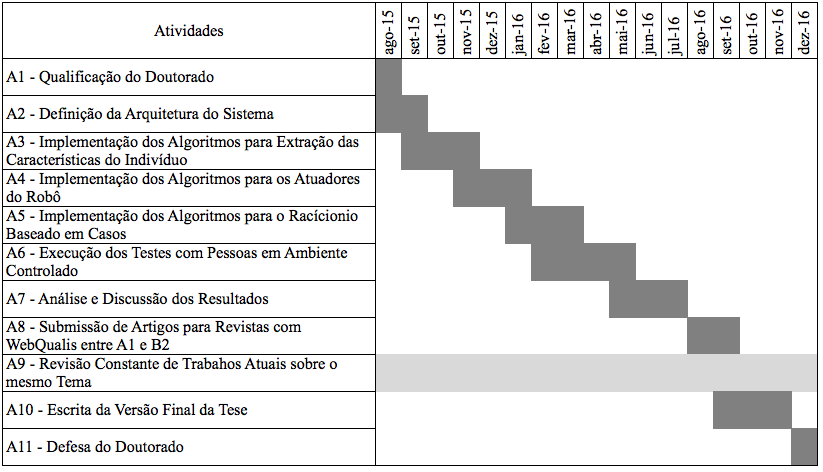
\includegraphics[width=\textwidth]{cronograma.png}
	\caption{Cronograma para Conclusão da Tese.}
	\label{fig:cronograma}
\end{figure}

A lista a seguir apresenta com mais detalhes as tarefas apresentadas no cronograma da figura~\ref{fig:cronograma}.

\begin{enumerate}
	\item \textbf{A1}: Apresentação do Exame de Qualificação para o Doutorado;
	\item \textbf{A2}: Definição da Arquitetura que irá auxiliar o desenvolvimento e execução do Sistema que poderá ser consumido por diferentes tipos de robô ao mesmo tempo;
	\item \textbf{A3}: Desenvolvimento dos algoritmos que serão utilizados para fazer com que o robô possa extrair as informações comportamentais das pessoas, de acordo com o apresentado na seção~\ref{sec:extracaocaracteristicas};
	\item \textbf{A4}: Desenvolvimento dos algoritmos que irão controlar os atuadores do robô, como por exemplo, cabeça, manipulador e motores;
	\item \textbf{A5}: Desenvolvimento dos algoritmos que compõem o mecanismo para Raciocínio Baseado em Casos, responsável pelo aprendizado de interação do robô;
	\item \textbf{A6}: Execução dos testes de interação de acordo com o descrito no capitulo~\ref{cap:testes};
	\item \textbf{A7}: Análise dos resultados utilizando métodos estatísticos e também as observações obtidas durante o acompanhamento dos testes de interação;
	\item \textbf{A8}: Submissão de pelo menos 2 artigos sobre a tese para revistas relevantes para a área de pesquisa, classificadas de acordo com o WebQualis da CAPES entre os níveis de A1 à B2;
	\item \textbf{A9}: Revisão bibliográfica contínua para certificar da originalidade e atualidade do trabalho de tal forma, que sua contribuição possa ajudar o avanço da área de pesquisa em robótica social e assistiva;
	\item \textbf{A10}: Consolidação do trabalho no texto do documento da tese para entrega à banca avaliadora;
	\item \textbf{A11}: Apresentação da Defesa para o título de Doutor.
\end{enumerate}


% \bibliography{biblio}
\printbibliography
\end{document}
